\documentclass[a4paper,12pt,twoside]{book}
\usepackage[T1]{fontenc}
\usepackage{inputenc}
\usepackage{fontspec}
\usepackage{lmodern}
\usepackage[english,french]{babel}

% Paquets pour le chinois
\usepackage{xeCJK}
\setCJKmainfont{Noto Sans CJK SC}
\usepackage[overlap,CJK]{ruby}
\usepackage{xpinyin}

\usepackage{xspace} % pour la gestion des espaces après les commandes
\usepackage{minted} % colored source code
\usepackage{csquotes}

% Mise en page École des chartes
\usepackage[margin=2.5cm]{geometry} % marges
\usepackage{setspace}
\onehalfspacing % interligne de 1.5
\setlength\parindent{1cm}

\usepackage{graphicx}
\usepackage{tabularx}
\usepackage{lscape}
\usepackage{pdfpages}
\usepackage{pdflscape}

\usepackage[backend=biber, sorting=nyt, style=enc, minbibnames=10, maxbibnames=10]{biblatex}
\addbibresource{bibliographie/bibliographie.bib}
\nocite{*}
\defbibnote{intro}{Cette bibliographie présente toutes les ressources utilisées, de tout type, citées ou non, par simple ordre alphabétique.}


\usepackage[pdfusetitle, pdfsubject={Mémoire TNAH — Titre}, pdfkeywords={mot1, mot2, mot3}]{hyperref}

\author{Maëva Nguyen – M2 TNAH — ENC}
\title{Titre mémoire}

% ACRONYMS
\usepackage[automake, acronym, toc]{glossaries}
\makeglossaries
\setacronymstyle{short-long}
\newacronym{fair}{\textsc{FAIR}}{\emph{Findable Accessible Interoperable Reusable}}
\newacronym{COREL}{\textsc{COREL}}{\emph{Code relationnel}}
\newacronym{EFEO}{\textsc{EFEO}}{\emph{École Française d'Extrême-Orient}}
\newacronym{IHEC}{\textsc{IHEC}}{\emph{Institut des hautes études chinoises}}
\newacronym{CollEx}{\textsc{CollEx}}{\emph{Collections d'excellence}}
\newacronym{EPHE}{\textsc{EPHE}}{\emph{École pratique des hautes études}}
\newacronym{EHESS}{\textsc{EHESS}}{\emph{École des hautes études en sciences sociales}}
\newacronym{IR}{\textsc{IR}}{\emph{Infrastructure de recherche}}
\newacronym{LSC}{\textsc{LSC}}{\emph{Legalizing space in China}}
\newacronym{EPJ}{\textsc{EPJ}}{\emph{Emerging procedural justice}}
\newacronym{POC}{\textsc{POC}}{Proof of concept}
\newacronym{ANR}{\textsc{ANR}}{\emph{Agence nationale de la recherche}}
\newacronym{XML}{\textsc{XML}}{\emph{Extensible Markup Language}}
\newacronym{IIIF}{\textsc{IIIF}}{\emph{International image interoperability framework}}
\newacronym{JSON}{\textsc{JSON}}{\emph{JavaScript Object Notation}}
\newacronym{SQL}{\textsc{SQL}}{\emph{Structured Query Language}}
\newacronym{SGBD}{\textsc{SGBD}}{\emph{Système de gestion de base de données}}
\newacronym{IDE}{\textsc{IDE}}{\emph{Integrated development environment}}
\newacronym{FTP}{\textsc{FTP}}{\emph{File Transfer Protocole}}
\newacronym{HTML}{\textsc{HTML}}{\emph{HyperText Markup Language}}
\newacronym{ODD}{\textsc{ODD}}{\emph{One Document Does It All}}
\newacronym{TEI}{\textsc{TEI}}{\emph{Text Encoding Initiative}}
\newacronym{DTD}{\textsc{DTD}}{\emph{Document Type Definition}}
\newacronym{OCR}{\textsc{OCR}}{\emph{Optical Character Recognition}}
\newacronym{UML}{\textsc{UML}}{\emph{Unified Modeling Language}}
\newacronym{XSL}{\textsc{XSL}}{\emph{Extensible Stylesheet Language}}
\newacronym{CSV}{\textsc{CSV}}{\emph{Coma Separated Values}}
\newacronym{PDF}{\textsc{PDF}}{\emph{Portable Document Format}}
\newacronym{TSV}{\textsc{TSV}}{\emph{Tab Separated Values}}
\newacronym{OAI-PMH}{\textsc{OAI-PMH}}{\emph{Open Archives Initiative Protocole for Metadata Harvesting}}
\newacronym{XSLT}{\textsc{XSLT}}{Extensible Stylesheet Language Transformation}
\newacronym{JS}{\textsc{JS}}{\emph{JavaScript}}
\newacronym{W3C}{\textsc{W3C}}{\emph{World Wide Web Consortium}}
\newacronym{DiScholEd}{\textsc{DiScholEd}}{\emph{Digital Scholarly Editions}}
\newacronym{XPath}{\textsc{XPath}}{\emph{XML Path Language}}

% COMMANDS
\newcommand{\enc}{École nationale des chartes\xspace}
\newcommand{\fair}{\gls{fair}\xspace}
\newcommand{\api}{\gls{api}\xspace}
\newcommand{\XIV}{\textsc{xiv}\ieme{}\xspace}
\newcommand{\COREL}{\gls{COREL}\xspace}
\newcommand{\cdf}{Collège de France\xspace}
\newcommand{\EFEO}{\gls{EFEO}\xspace}
\newcommand{\IHEC}{\gls{IHEC}\xspace}
\newcommand{\CollEx}{\gls{CollEx}\xspace}
\newcommand{\EPHE}{\gls{EPHE}\xspace}
\newcommand{\EHESS}{\gls{EHESS}\xspace}
\newcommand{\IR}{\gls{IR}\xspace}
\newcommand{\LSC}{\gls{LSC}\xspace}
\newcommand{\EPJ}{\gls{EPJ}\xspace}
\newcommand{\code}{\og code virtuel \fg \xspace}
\newcommand{\POC}{\gls{POC}\xspace}
\newcommand{\ANR}{\gls{ANR}\xspace}
\newcommand{\XML}{\gls{XML}\xspace}
\newcommand{\IIIF}{\gls{IIIF}\xspace}
\newcommand{\JSON}{\gls{JSON}\xspace}
\newcommand{\genyuan}{\textit{Da Qing lüli genyuan}\xspace}
\newcommand{\huidian}{\textit{Huidian shili}\xspace}
\newcommand{\dc}{\textit{Duli cunyi}\xspace}
\newcommand{\dq}{\textit{Da Qing lüli}\xspace}
\newcommand{\dqlj}{\textit{Da Qing lü jijie fuli\xspace}}
\newcommand{\SQL}{\gls{SQL}\xspace}
\newcommand{\SGBD}{\gls{SGBD}\xspace}
\newcommand{\IDE}{\gls{IDE}\xspace}
\newcommand{\FTP}{\gls{FTP}\xspace}
\newcommand{\HTML}{\gls{HTML}\xspace}
\newcommand{\ODD}{\gls{ODD}\xspace}
\newcommand{\TEI}{\gls{TEI}\xspace}
\newcommand{\lu}{\textit{lü}\xspace}
\newcommand{\li}{\textit{tiaoli}\xspace}
\newcommand{\DTD}{\gls{DTD}\xspace}
\newcommand{\cv}{\og code virtuel \fg}
\newcommand{\tp}{\textit{TEI Publisher}\xspace}
\newcommand{\OCR}{\gls{OCR}\xspace}
\newcommand{\UML}{\gls{UML}\xspace}
\newcommand{\XSL}{\gls{XSL}}
\newcommand{\cordel}{\textit{Démêler le Cordel}\xspace}
\newcommand{\calendar}{\textit{Chinese Calendar Tools}\xspace}
\newcommand{\csv}{\gls{CSV}\xspace}
\newcommand{\pdf}{\gls{PDF}\xspace}
\newcommand{\tsv}{\gls{TSV}\xspace}
\newcommand{\oai}{\gls{OAI-PMH}\xspace}
\newcommand{\XSLT}{\gls{XSLT}\xspace}
\newcommand{\JS}{\gls{JS}\xspace}
\newcommand{\w}{\gls{W3C}\xspace}
\newcommand{\disco}{\gls{DiScholEd}\xspace}
\newcommand{\xpath}{\gls{XPath}\xspace}

% Pour retirer le titre courant d'une page vide avant un chapitre
\newcommand{\clearemptydoublepage}{\newpage{\pagestyle{empty}\cleardoublepage}}
% Pour des sections non numérotées dans la table des matière
\newcommand\chapterNo[1]{
  \chapter*{#1}
  \markright{\MakeUppercase{#1}}
}

\begin{document}

\onehalfspacing 

\frontmatter

    \begin{titlepage}
    \begin{center}
        
        \bigskip
        
        \begin{large}
            ÉCOLE NATIONALE DES CHARTES
        \end{large}
        \begin{center}\rule{2cm}{0.02cm}\end{center}
        
        \bigskip
        \bigskip
        \bigskip
        \begin{Large}
            \textbf{Maëva Nguyen}\\
        \end{Large}
        \begin{normalsize} \textit{licenciée ès lettres}\\
        \end{normalsize}
        
        \bigskip
        \bigskip
        \bigskip
        
        \begin{Huge}
            \textbf{Préparation des données pour l'édition scientifique numérique}\\
        \end{Huge}
        \bigskip
        \bigskip
        \begin{LARGE}
            \textbf{Contribuer à l'ouverture des données de la recherche}\\
        \end{LARGE}
        
        \bigskip
        \bigskip
        \bigskip
        \begin{large}
        \end{large}
        \vfill
        
        \begin{large}
            Mémoire 
            pour le diplôme de master \\
            \og Technologies numériques appliquées à l'histoire~\fg\\
            \bigskip
            2023
        \end{large}
        
    \end{center}
\end{titlepage}


    \thispagestyle{empty}	
    \cleardoublepage
	
    \chapterNo{Résumé}
\addcontentsline{toc}{chapter}{Résumé}
\medskip	

Résumé\\

\textbf{Mots-clés~:} mot1~; mot2~; mot3~.\\

\textbf{Informations bibliographiques~:} Maëva Nguyen, \textit{Titre du mémoire}, mémoire de master \og Technologies numériques appliquées à l'histoire~\fg, dir. Ségolène Albouy, École nationale des chartes, 2023.

\clearemptydoublepage
	
    \chapterNo{Remerciements}
    \addcontentsline{toc}{chapter}{Remerciements}
    
    \chapterNo{Introduction}
    L'édition scientifique numérique fait l'objet de nombreux projets de recherche. La publication de textes en ligne permet de diffuser des sources, notamment historiques et littéraires, à un plus large public - chercheurs, étudiants ou non-spécialistes. En plus de servir la valorisation des sources, cette diffusion massive de textes en ligne contribue au concept de l'\textit{open data}, un concept clef des humanités numériques : permettre l'accès et la réutilisation des données de la recherche par tous, en respectant les droits d'auteurs. 

Les enjeux de la diffusion des données de la recherche sont aujourd'hui doubles : aux enjeux patrimoniaux s'ajoutent désormais ceux de la science ouverte, introduits par l'usage du numérique au service de la recherche. Plus qu'un outil, l'union du numérique et de la recherche permet à des projets pluri-disciplinaires de voir le jour. Ainsi, les chercheurs en histoire agrandissent leur champ de compétences en travaillant conjointement avec des ingénieurs en humanités numériques. 

L'édition scientifique numérique répond à deux besoins majeurs de la recherche : préserver les sources originales tout en valorisant leur contenu. Créer des sources numériques et les publier permet ainsi de démocratiser l'accès aux ressources, disponibles en libre accès. Cependant, cette affluence de données sur le web pose la question des \og bonnes pratiques \fg de la science ouverte. Diffuser librement des données sur le web requiert également de respecter les principes \fair des données pour assurer l'utilité d'une telle entreprise. Pour aider à la mise en place de l'\textit{open data}, le \w indique des standards à respecter afin de garantir l'accessibilité des données sur le web. 

%annonce de problématique/plan
Le projet \COREL est représentatif de ces enjeux pluri-disciplinaires : son équipe cherche à assurer la valorisation d'un corpus de textes et l'accès à ces sources via le numérique, en s'inscrivant dans cette démarche de science ouverte. À travers l'étude de ce projet et de ces enjeux, il est pertinent de se demander en quoi l’édition scientifique numérique peut offrir aux chercheurs un accès facilité à des informations dispersées dans différentes sources. Il est également intéressant d'explorer comment le numérique permet de retracer l’évolution de la législation de la Chine impériale année après année et assurer la cohérence d’un code légal reconstitué à partir de sources partielles. Après une présentation du projet et de ses objectifs, l'analyse de l'étape de préparation des données conformément au standard \TEI et la diffusion de ces données sur le web seront le moyen d'évoquer comment un projet de recherche peut contribuer à l'\textit{open data} grâce au numérique.
    \addcontentsline{toc}{chapter}{Introduction}

    \thispagestyle{empty}
    \cleardoublepage

\mainmatter

    \part{Le projet COREL, un projet de recherche inter-institutionnel}
        \chapter{Le projet COREL}
        Le projet \COREL est un projet de recherche inter-institutionnel entre le \cdf et l'\EFEO. Ce projet pluridisciplinaire réunit les humanités numériques et l'histoire du droit chinois et initie ainsi la collaboration entre historiens du droit, sinologues et ingénieurs en sciences humaines.
                    \section{La collaboration entre les institutions}
\subsection{Le Collège de France}

\subsubsection{Historique}
Le \cdf naît sous le règne de François I\ier{} lorsqu'en 1520, Guillaume Budé, libraire du roi, demande la création d'une institution regroupant des professeurs. C'est ainsi que sont nommés trois professeurs d'hébreux, deux de grec et un de mathématiques en 1530 par François I\ier{} : les lecteurs royaux. La création du \cdf est issue de la croissance de l'humanisme et, en accord avec sa devise \textit{\og Docet omnia \fg}, il enseigne \og tout \fg. C'est d'abord une institution "bâti[e] en hommes", comme le dit Pierre Bayle, qui ne possède pas de siège. Cependant, les cours ont essentiellement lieu place de Cambrai, et un bâtiment y est construit à la fin du XVIII\ieme siècle. Aujourd'hui encore, les cours donnés au \cdf sont publics et ouverts à tous. L'institution s'inscrit ainsi dans une tradition de \og science ouverte \fg. 

\subsubsection{Organisation actuelle}
Le \cdf est divisé en plusieurs chaires. Les chaires statutaires sont attribuées à des professeurs élus, qui occupent cette position jusqu'à l'âge de 73 ans. Les chaires annuelles et internationales sont occupées par des chercheurs choisis par l'Assemblée du \cdf pour des périodes plus courtes. En plus des cours ouverts à tous publics et donnés sur place, le \cdf met à disposition des cours en ligne, des enregistrements, des podcasts, etc. afin de diffuser le savoir plus librement via leur site internet et une chaîne YouTube. 

\subsubsection{La bibliothèque d'études chinoises}
La Bibliothèque d'études chinoise du \cdf a été fondée en 1927 par Paul Pelliot et Marcel Granet. Elle est rattachée à l'\IHEC, lui-même fondé en 1920. La bibliothèque de l'\IHEC rejoint le \cdf en 1972. Elle possède un fonds de 120 000 oeuvres, dont 1 600 périodiques, principalement de la Chine impériale et pré-impériale. Cette collection a reçu le label \CollEx en 2021. La bibliothèque met à la disposition du projet \COREL des sources juridiques et leurs numérisations. Elle est le porteur administratif du projet.

\subsection{L’École Française d'Extrême-Orient}

\subsubsection{Historique}
L'\EFEO a été créée en 1898 à Hô Chi Minh-Ville (aussi appelée Saigon) sous le nom de \og Mission archéologique d'Indo-Chine \fg. L'institution naît sous l'influence du courant orientaliste du XIX\ieme siècle en France, afin d'encourager les chercheurs à se rendre en Indo-Chine, et celle du gouvernement d'Indo-Chine, pour préserver le patrimoine indo-chinois. La \og Mission archéologique d'Indo-Chine \fg devient l'\EFEO en 1900.

\subsubsection{Organisation actuelle}
L'\EFEO se situe dans le 16\ieme arrondissement de Paris, au sein de la Maison de l'Asie, un bâtiment partagé avec l'\EPHE et l'\EHESS. L'\EFEO compte dix-huit centres de recherche en Asie, notamment à Pondichéry, Hanoi ou encore Jakarta. Les chercheurs en sciences humaines et sociales de l'\EFEO étudient les civilisations asiatiques à travers un champ pluridisciplinaire (histoire, philologie, sciences de la religion, archéologie...). L'\EFEO collabore avec le \cdf pour le projet \COREL. 

\subsection{Les infrastructures de recherche (l'\IR* Huma-Num et Data Futures)}
\subsubsection{L'\IR* Huma-Num}
L'\IR* Huma-Num est une infrastructure de recherche dans le domaine des humanités numériques et accompagne les chercheurs en sciences humaines. Elle prend appui sur les principes \fair des données et la science ouverte. Son objectif est de permettre aux chercheurs d'accéder librement aux données de la recherche, mais aussi de garantir leur pérennité et leur qualité. 

L'\IR* Huma-Num est partenaire du projet \LSC dont est issu le projet \COREL. 

\subsubsection{Data Futures}
Data Futures est une entreprise à but non-lucratif qui aide à la préservation et à l'accessibilité des données de la recherche. Elle participe à des projets d'humanités numériques à travers les sciences de la vie et les sciences humaines et sociales.

Elle est partenaire du projet \COREL et du projet précédent \EPJ. Le projet fait appel à ses prestations de manière ponctuelle pour le traitement des données.

\section{Présentation du projet \COREL}
\subsection{Description du projet}
Le projet \COREL est un projet de recherche en humanités numériques, qui vise à reconstituer l'histoire du droit de la Chine impériale tardive sous la dynastie Qing (1644 - 1911). Ce projet prend appui sur deux projets précédents, les projets \LSC et \EPJ, auxquels le responsable scientifique du projet, M. Frédéric Constant, a également participé. À partir des sources juridiques de la bibliothèque des hautes études chinoises, de leur édition en ligne par le projet \LSC et des numérisations et annotations des sources par le projet \EPJ, le projet \COREL propose à la fois une édition en ligne des textes de lois et une reconstitution de sources partielles grâce au numérique

Le projet a obtenu un financement \CollEx-Persée pour deux ans, jusqu'au mois d'octobre 2024. 

\subsection{L’objectif du projet}
Le projet \COREL a pour objectif de préserver et valoriser un corpus de sources historiques du droit chinois et de les mettre à la disposition des chercheurs, qu'ils soient historiens du droit ou sinologues. Proposer l'agrégation de ces sources partielles et qui se complètent les unes les autres pour faciliter le travail des chercheurs est au c\oe ur de ce projet, c'est pourquoi seuls des outils open-source et bien documentés, consacrés à la publication scientifique numérique et appuyés par une communauté de chercheurs en humanités numériques, sont envisagés pour réaliser les livrables.

\subsection{Les livrables du projet}
Plusieurs livrables sont attendus pour la fin du financement \CollEx-Persée en 2024. Le premier livrable est un site internet qui recrée partiellement celui du projet \LSC en proposant une édition scientifique numérique des codes légaux ainsi que des compilations des codes.
Une fonctionnalité appelée \code sera intégrée au site web afin de reconstituer la législation chinoise entre 1644 et 1911. Ce \code permet de recréer artificiellement la législation à partir l'agrégation des différentes sources du corpus. Pour une année donnée, l'utilisateur pourra consulter toutes les lois en vigueur, ordonnées selon les normes de composition d'un code légal sous la dynastie Qing (divisions en chapitres, lois secondaires classées sous la loi principale à laquelle elles sont rattachées...)

Le projet souhaite aussi intégrer des visualisations permettant de retracer la généalogie d'une loi, sa promulgation, ses modifications et éventuellement ses fusions, divisions ou encore abrogations lorsqu'elles existent. Ces visualisations seront accessibles directement depuis l'édition en ligne, en cliquant sur le titre de la loi dont l'utilisateur souhaite consulter la généalogie. 

Soumis à un financement limité dans le temps, le projet \COREL s'engage auprès de \CollEx-Persée à fournir un \POC de ces livrables, sur un jeu de données réduits si le temps ne permet pas la réalisation de tous ces livrables. Trois lois seront choisies pour représenter le corpus dans son intégralité, avec des cas de figures complexes permettant d'illustrer la faisabilité de la reconstitution de la législation chinoise impériale.


\section{Les projets de recherche antérieurs}
\subsection{Le projet Legalizing space in China}

Le projet \LSC a reçu un financement de l'\ANR de 2011 à 2015. L'objectif de ce projet est de réunir les sources du droit chinois (mais également d'autres pays d'Asie : Mongolie, Corée, Japon, Vietnam) dans une édition en ligne trilingue (chinois, français et anglais). 

Le site web du projet \LSC réunit donc un grand nombre d'éditions en ligne de codes légaux et de compilations, ainsi que leurs numérisations au format PDF. \LSC propose également des tableaux synoptiques des codes, un glossaire qui permet à la fois l'étude des termes juridiques chinois, mais aussi l'harmonisation du travail de traduction, un index des noms de lieux et de personnes et des cartes de la Chine en relation avec les textes de lois. 

Le projet \COREL s'appuie sur une partie des sources utilisées par le projet \LSC et leur édition numérique. Cette édition a été réalisée grâce à des documents encodés en \XML. Ces sources numériques sont reprises dans le cadre du projet \COREL comme socle à la création d'un nouveau jeu de données pour la publication en ligne. 

\subsection{Le projet Emerging procedural justice}
Le projet \EPJ a obtenu un financement Arqus European University Alliance en 2020. Ce projet s'est effectué en collaboration avec la société Data Futures et a permis de déposer sur un serveur \IIIF les numérisations des sources, puis de les annoter et les segmenter pour mettre en avant la structure des textes ainsi que les relations qui existent entre les lois. Ces annotations ont été réalisées à partir d'un fichier de recensement exhaustif des relations entre les lois des différents codes. 

Dans le cadre du projet \COREL, l'export de ces numérisations au format \JSON sont utilisées pour enrichir le jeu de données du projet et retracer la généalogie des lois.  
            
            
        \clearemptydoublepage
        
        \chapter{Le corpus}
        Le projet \COREL s'inscrit dans un champ disciplinaire particulier, au croisement de la sinologie et de l'histoire du droit. Développer l'accès à des ressources encore peu diffusées dans le domaine des humanités numériques constitue un enjeu majeur du projet. 
                    \section{Contexte historique}
    \subsection{La Chine impériale sous la dynastie Qing}

Le projet \COREL vise à étudier l'évolution du droit lors de la période de la Chine impériale tardive, de 1644 à 1911. Ces bornes chronologiques correspondent au règne de la dynastie Qing. En effet, les Qing, venant de Mandchourie, renversent la dynastie Ming (1368-1644) en prenant la capitale, Pékin. La dynastie Qing règne alors avec l'empereur Shunzhi (1644 - 1661) au pouvoir, lequel opère la transition entre les deux dynasties. Il fait éditer le premier code légal des Qing, le \dqlj, qui hérite directement du code des Ming, révisé pour la nouvelle dynastie. La modification du code légal de la dynastie précédente, selon Zheng Qin et Guangyuan Zhou, s'explique ainsi : 

\begin{quote}
    Indeed, the relatively smooth transition
 from the Ming code to the Qing code needs some explanation. The
 Ming code represented the highest legislative achievement in tradi-
 tional China, making the new rulers reluctant to abandon it. Further-
 more, the Manchu rulers had already familiarized themselves with the
 Ming law and political system before they conquered China. \footnote{\cite{qin_pursuing_1995}}
\end{quote}
C'est donc dans la continuité directe du code des Ming que va s'écrire le code légal des Qing.

Après Shunzhi, c'est l'empereur Kangxi (1662-1722) qui est à la tête du pays. Son règne se caractérise par une certaine ouverture aux sciences occidentales via des jésuites, venus en Chine pour transmettre leurs savoirs et tenter d'évangéliser la Chine. L'empire Mandchou s'étend progressivement jusqu'au milieu du XVIII\ieme siècle. Deux autres grands empereurs succèdent à Kangxi : Yongzheng (1723 - 1735) et Qianlong (1736 - 1795). En 1911, la dynastie Qing est remplacée par un gouvernement républicain.

\subsection{La législation chinoise et l’édition des codes légaux}

Les textes de lois chinois relèvent majoritairement du droit pénal et observent une structure définie et rigoureuse. Sous la dynastie des Qing, les codes légaux se divisent en sept chapitres majeurs (appelés \textit{bu}), structure déjà employée pour les textes de lois de la dynastie précédente. En effet, le code des Ming de 1397 utilise cette division en sept chapitres, dont les codes des Qing héritent. Le premier chapitre contient des propos généraux (\og Dénominations et règles \fg \footnote{Les titres de chapitres, entre guillemets, sont empruntés à la traduction proposée par le projet \LSC.}) et les six chapitres suivants sont organisés selon les six ministères (la division du gouvernement en ces six ministères étant observée depuis la dynastie Tang \footnote{Dynastie régnante en Chine de 618 à 907}) : \og Lois administratives \fg, \og Lois domestiques \fg, \og Lois rituelles \fg, etc. À l'instar du code des Ming, ces chapitres sont ensuite divisés en trente sections (en chinois \textit{men}), par exemple \og Institutions administratives \fg, \og Documents officiels \fg, etc. 

Ces chapitres et sections contiennent deux types de lois. Les lois dites principales, les \lu, sont des lois fixes qui constituent la colonne vertébrale du code des Qing (en anglais \textit{statutes}). Certaines lois principales sont directement héritées de la législation de la dynastie Tang, ou ont subi des changements mineurs de vocabulaire. Selon Derk Bodde et Clarence Morris, fixer des lois immuables d'une dynastie à l'autre relèverait d'une vision morale de la loi en Chine : 
\begin{quote}
    No doubt this continuity reflects the Chinese view of law as the codification of moral truths retaining eternal validity irrespective of time or place. \footnote{\cite{law_in_imperial_china}}
\end{quote}

Toutefois, ce propos est nuancé dans leur ouvrage puisque, de fait, moins de la moitié des lois principales demeurent véritablement immuables. Les autres \lu sont modifiées, parfois supprimées ou même créées sous la dynastie Qing, jusqu'en 1740, année de leur dernière version. De plus, les \lu sont accompagnées d'articles additionnels (ou lois secondaires), les \li (aussi appelées \textit{li}, ou en anglais \textit{substatutes}). Les lois secondaires sont des ajouts aux lois principales. Loin d'être figées, elles traitent du droit vivant et viennent préciser la loi principale à laquelle elles sont rattachées. Elles apparaissent souvent à la suite de jugements ou de cas particuliers. Les lois principales ont tendance à se réduire avec le temps. Elles sont au nombre de 436 en 1740. En revanche, les \li augmentent au fur et à mesure. Il en existe une centaine en 1740. À la fin du XIX\ieme siècle, on compte plus de 1 000 lois secondaires. 

 \section{Des sources juridiques}
    \subsection{Les éditions du code légal (1646, 1740)}

Les codes légaux des Qing sont révisés et publiés de manière plus ou moins régulière, tous les dix ans environ. Entre 1740 et 1871, date de la dernière édition du code, on compte 23 rééditions. Toutefois, toutes ces rééditions n'ont pas été conservées, ce qui laisse le corpus incomplet. Dans le cadre du projet \COREL, deux éditions du code légal sont utilisées. 

En 1646, la première édition du code légal des Qing, \dqlj, compte une centaine d'articles. Cette première édition du code s'inscrit dans la continuité du code de la dynastie Ming. Les historiens, notamment Tan Qian  qui a connu les deux dynasties, critiquent cette première édition du code qui n'a pratiquement rien de nouveau et ressemble très fortement au code des Ming. 

La seconde édition du code des Qing intégrée au corpus du projet est le code de 1740, \dq. Dans cette version du code, les \lu sont définitivement établies et ne sont plus modifiées. Comme son nom l'indique, ce texte met sur le même plan les lois principales, \lu et les lois secondaires, \li. En effet, sous la dynastie Ming, les \li n'étaient que des exemples aux lois principales. Elles prennent de plus en plus d'ampleur dans le droit chinois, jusqu'à avoir véritablement la même importance que les lois principales en 1740.

Néanmoins, ces éditions du codes, largement espacées, ne reflètent la loi qu'au moment où elles sont produites et ne prennent pas en compte les modifications qu'il y a pu y avoir entre deux éditions. C'est pourquoi, en plus des éditions des codes légaux, d'autres sources viennent nourrir le projet \COREL : des compilations des textes de lois, qui viennent compléter les zones d'ombres que laissent les codes légaux.

\subsection{Les compilations des textes de loi}

Les compilations des textes de lois sous la dynastie Qing ont une structure similaire à celle des codes légaux et suivent la structure rigoureuse en sept chapitres. Toutefois, ces documents présentent également des caractéristiques qui leur sont propres et viennent compléter les codes légaux. 

En 1871, le \genyuan est publié. Il présente les articles additionnels dans l'ordre chronologique, c'est-à-dire dans l'ordre de modification du code légal. Le \huidian paraît en 1899 et compile l'ensemble des lois en vigueur mais aussi les lois abrogées. Enfin, le \dc est un texte de 1905 qui compile toutes les lois en vigueur sous la dynastie des Qing, avec des explications historiques. Cette compilation a été établie par Xue Yuncheng pour aider à la révision du code légal. Ces trois textes sont des sources qui viennent compléter les textes légaux grâce à leur exhaustivité en présentant toutes les modifications et abrogations des lois et permettent d'en retracer la généalogie.

En plus de ces textes, il existe des recueils de cas qui expliquent l'origine des lois. En effet, les articles additionnels résultent de jugements ou de cas particuliers, il est donc possible de retracer l'origine d'une loi à une affaire, un décret ou un fonctionnaire. Toutefois, ces documents ne font pas partie du projet \COREL. Actuellement en cours de numérisation par la bibliothèque d'études chinoises, les informations supplémentaires que peuvent apporter ces sources constituent une perspective d'enrichissement des données du projet qui sera envisagée à termes. 


\section{Les sources numériques}
    \subsection{Les documents \XML}
Le projet \COREL dispose de sources numériques issues des projets précédents. Ces sources ont été pensées et produites pour deux projets différents et ne sont pas liées entre elles. La source de données principale du projet provient du projet \LSC, qui offre une édition en ligne des sources balisées en \XML. 

\subsubsection{Encodage et validation des données}
Ce balisage \XML relève d'un schéma personnalisé, créé spécifiquement pour le projet \LSC. Pour comprendre ce balisage, il est indispensable de consulter en regard l'édition \XML et le site web du projet, qui sont étroitement liés. En effet, le balisage reprend la structure des codes légaux, familière aux chercheurs, mais lie ce balisage à l'affichage \HTML. Ainsi, certaines portions des textes sont balisées ainsi : 
\begin{minted}{xml}
<p>笞刑五:
    <inf>笞者,擊也,又訓為恥。用小竹板。</inf>一十;
    <inf>折四板。</inf>二十;<inf>除零,折五板。</inf>三十;
    <inf>除零,折一十板。</inf>四十;
    <inf>除零,折一十五板。</inf>五十;
    <inf>折二十板。</inf>
</p>
\end{minted}

En comparant ce code \XML à l'affichage du site, il est possible d'établir clairement le lien entre l'encodage et l'affichage : la balise \texttt{<inf/>} permet d'afficher une partie des paragraphes en caractères bleus, dans une police légèrement inférieure. 
\begin{figure}[h]
    \centering
    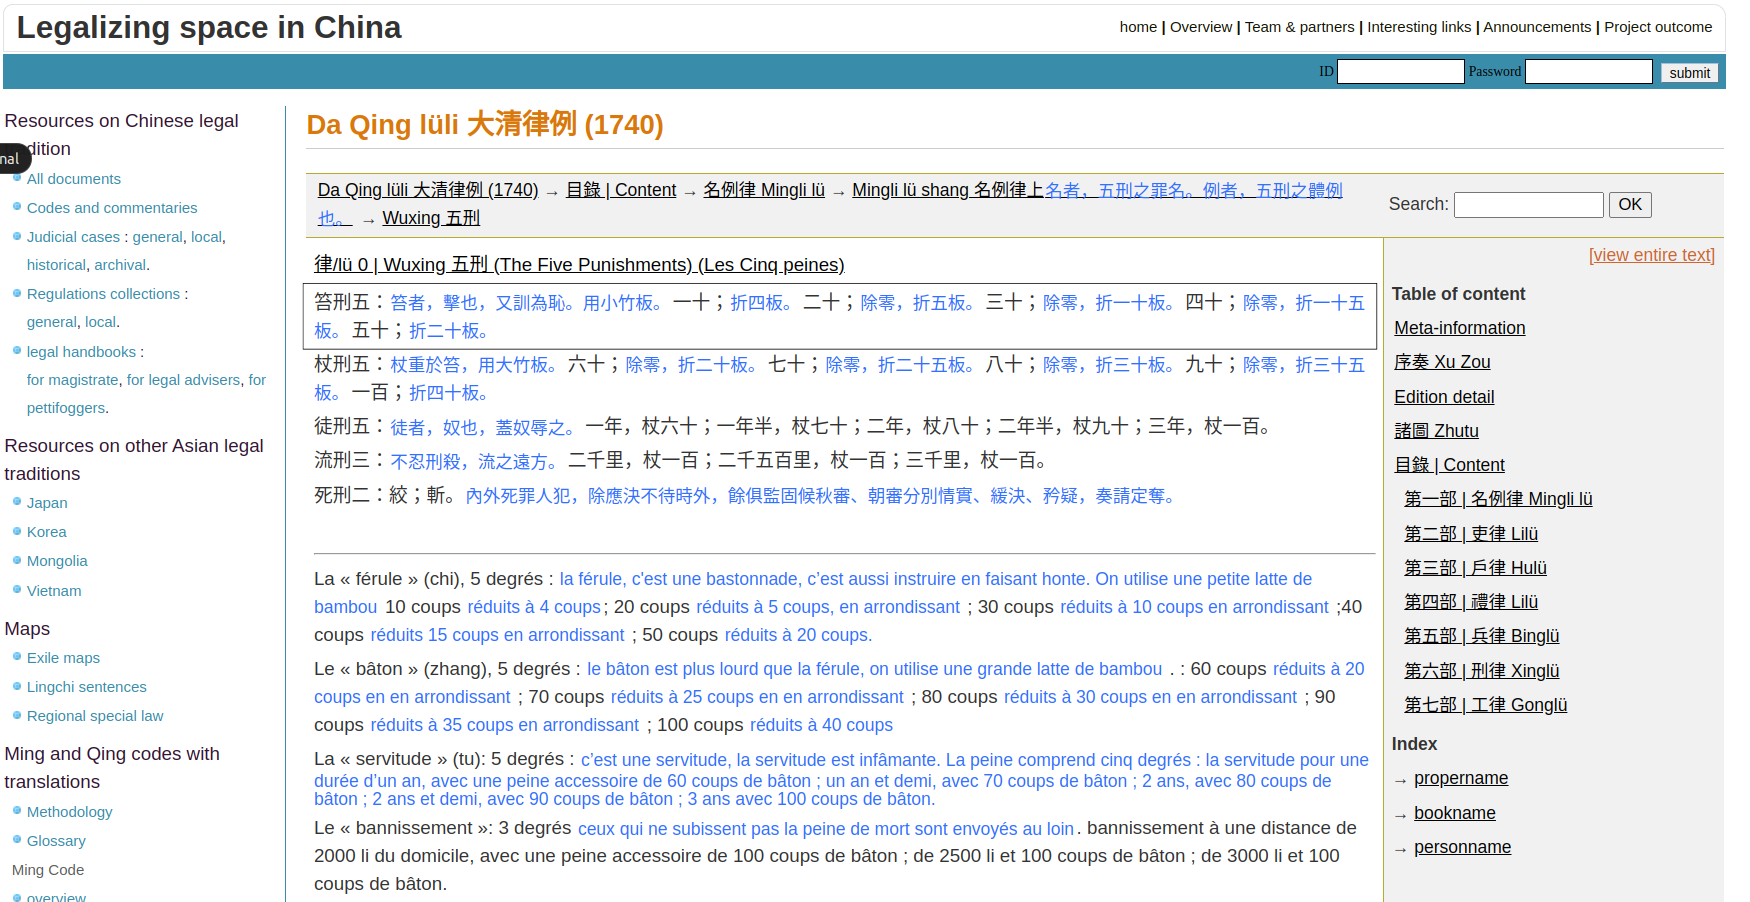
\includegraphics[width=\textwidth]{images/image1.png}
    \caption{Capture d'écran du site web \LSC - affichage du code \XML dans l'encadré.}
\end{figure}

Cette utilisation de l'encodage relève du mode de travail des chercheurs sur le projet. En effet, à partir de textes issus de l'\OCR, le texte est saisi et balisé dans le logiciel Oxygen au fur et à mesure du projet, c'est-à-dire que l'encodage des données et le développement du site s'effectuent en parallèle. Dès lors, le site web devient un outil de validation de la saisie des données : ce lien entre l'encodage et l'affichage permet aux chercheurs débutants en humanités numériques de vérifier leur code en mettant le site à jour, les erreurs d'affichages se repérant plus facilement qu'un oubli dans le code \XML. 

Mettre en parallèle les étapes d'encodage et de création du site internet relève du choix des chercheurs du projet d'utiliser un schéma \XML entièrement customisé. En effet, ce schéma n'est pas documenté et aucune \DTD n'a été produite pour valider l'encodage et contraindre ce schéma. Le projet \LSC continue aujourd'hui d'être alimenté par les chercheurs du projet \COREL. Dès lors, le seul moyen de se repérer dans un schéma sans documentation ni règles de validation devient l'affichage du site internet.

\subsubsection{Structure des sources numériques}
Sans documentation claire ni schéma de validation, comprendre la structure des sources numériques et les choix d'encodage est une étape essentielle du projet. En effet, il est difficile de comprendre au premier coup d'oeil le schéma utilisé pour encoder les sources sans avoir travaillé pour le projet \LSC et sans connaissances solides des textes de lois chinois. De plus, au fil du temps, les sources numériques ont été encodées par de nombreuses personnes, contribuant au projet \LSC ou bien au projet \COREL. L'encodage n'étant pas contraint et les objectifs des deux projets étant différents, les sources numériques ont parfois évolué et l'encodage des texte peut présenter des variantes d'encodage d'un texte à l'autre, voire au sein d'un même document. 

L'encodage \LSC prend comme point de départ la structure des sources originales en chapitres, sections, lois principales et secondaires, mais vient ajouter des éléments supplémentaires selon les spécificités de chaque document. Par exemple, le \huidian propose des listes de lois classées par année. Cet élément est propre à ce texte de lois et a nécessité un encodage différent, traduit par un élément \texttt{<enum>} contenant un ou plusieurs \texttt{<item>} et une balise \texttt{<date>}.

De plus, le projet \LSC est un projet d'édition scientifique numérique trilingue. Tous les documents ont donc été encodés en chinois, français et anglais. Chaque balise apparaît donc trois fois, avec un attribut de langue différent. 
\begin{minted}{xml}
    <title lang="ch">Wuxing 五刑</title>
    <title lang="en">The Five Punishments</title>
    <title lang="fr">Les Cinq peines</title>
\end{minted}
Toutefois, ces choix manquent d'uniformité dans l'encodage, car certaines balises ne sont pas triples et contiennent des informations hybrides entre plusieurs langues :
\begin{minted}{xml}
    <title lang="ch">目錄 | Content</title>
\end{minted}
D'autre part, la traduction des textes n'a jamais été achevée pendant le financement du projet \LSC. Il existe ainsi de nombreuses balises auto-fermantes dans l'encodage \XML, qui laissent la place à une traduction qui n'a pas de garantie de voir le jour, d'autant plus que le projet \COREL n'inclut pas les traductions dans son périmètre. 

Le trinlinguisme initial du projet \LSC semble à première vue être un élément que l'on peut aisément écarter du projet \COREL. Toutefois, il a des conséquences directes dans l'encodage. En effet, outre les nombreuses balises auto-fermantes qui rendent le code dense, il est possible d'observer une substitution progressive entre la balise \texttt{<content>} censée séparer les différentes traductions et la balise \texttt{<p>} qui permet de séparer les différents paragraphes. Puisque la balise \texttt{<content>} n'est pas effective dans le cadre du projet \COREL et systématiquement laissée vide pour le français et l'anglais, son utilisation première s'est parfois perdue et s'est substituée à la balise \texttt{<p>} lorsque le texte chinois ne contenait qu'un seul et unique paragraphe. 

Par ailleurs, le choix d'éditer des documents trilingues s'est aussi reflété dans la création du schéma d'encodage. Si les éléments les plus courants, comme les titres, possèdent des noms de balises en anglais, ce n'est pas le cas de la plupart des éléments structurants des sources. Ainsi, les chapitres sont balisés grâce à l'élément \texttt{<bu>}, les sections \texttt{<men>}, etc. Certaines balises viennent également rappeler le français, comme la balise \texttt{<inf>} qui vient signaler des caractères de police \textit{inférieure}. 

Tous ces éléments aboutissent à la création de sources numériques extrêmement spécifiques et viennent restreindre la communauté qui peut contribuer au projet ou en bénéficier, car seules quelques personnes possèdent toutes les clefs de compréhension pour déchiffrer ce support de travail. 

\subsection{La numérisation des codes légaux}
\subsubsection{\IIIF et annotations}
En plus des données produites par le projet \LSC, le projet \COREL hérite aussi des sources produites par le projet \EPJ. Les numérisations des textes de lois ont été déposées sur un serveur \IIIF géré par Data Futures. Les chercheurs ont ensuite accès à un visualiseur Mirador qui leur permet de segmenter les images pour expliciter la structure des codes légaux en chapitres, sections, \lu et \li. Cette segmentation permet de mettre en valeur un caractère annonçant le début d'une nouvelle partie. 

\newpage
\begin{figure}[h]
    \centering
    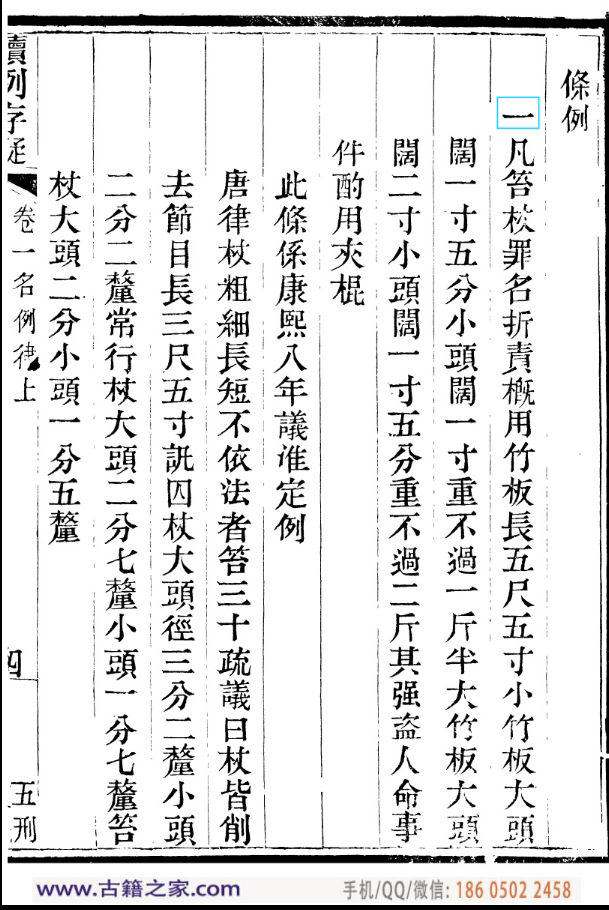
\includegraphics[width=100mm]{images/image2.png}
    \caption{Numérisation du \dc, segmentation du début du \li 1-1}
\end{figure}

Ces caractères qui marquent le début d'un élément structurant du document ont ensuite été annotés par les chercheurs. Le prestataire a mis en place un tableau à remplir pour annoter les passages segmentés. 

\begin{figure}[h]
    \centering
    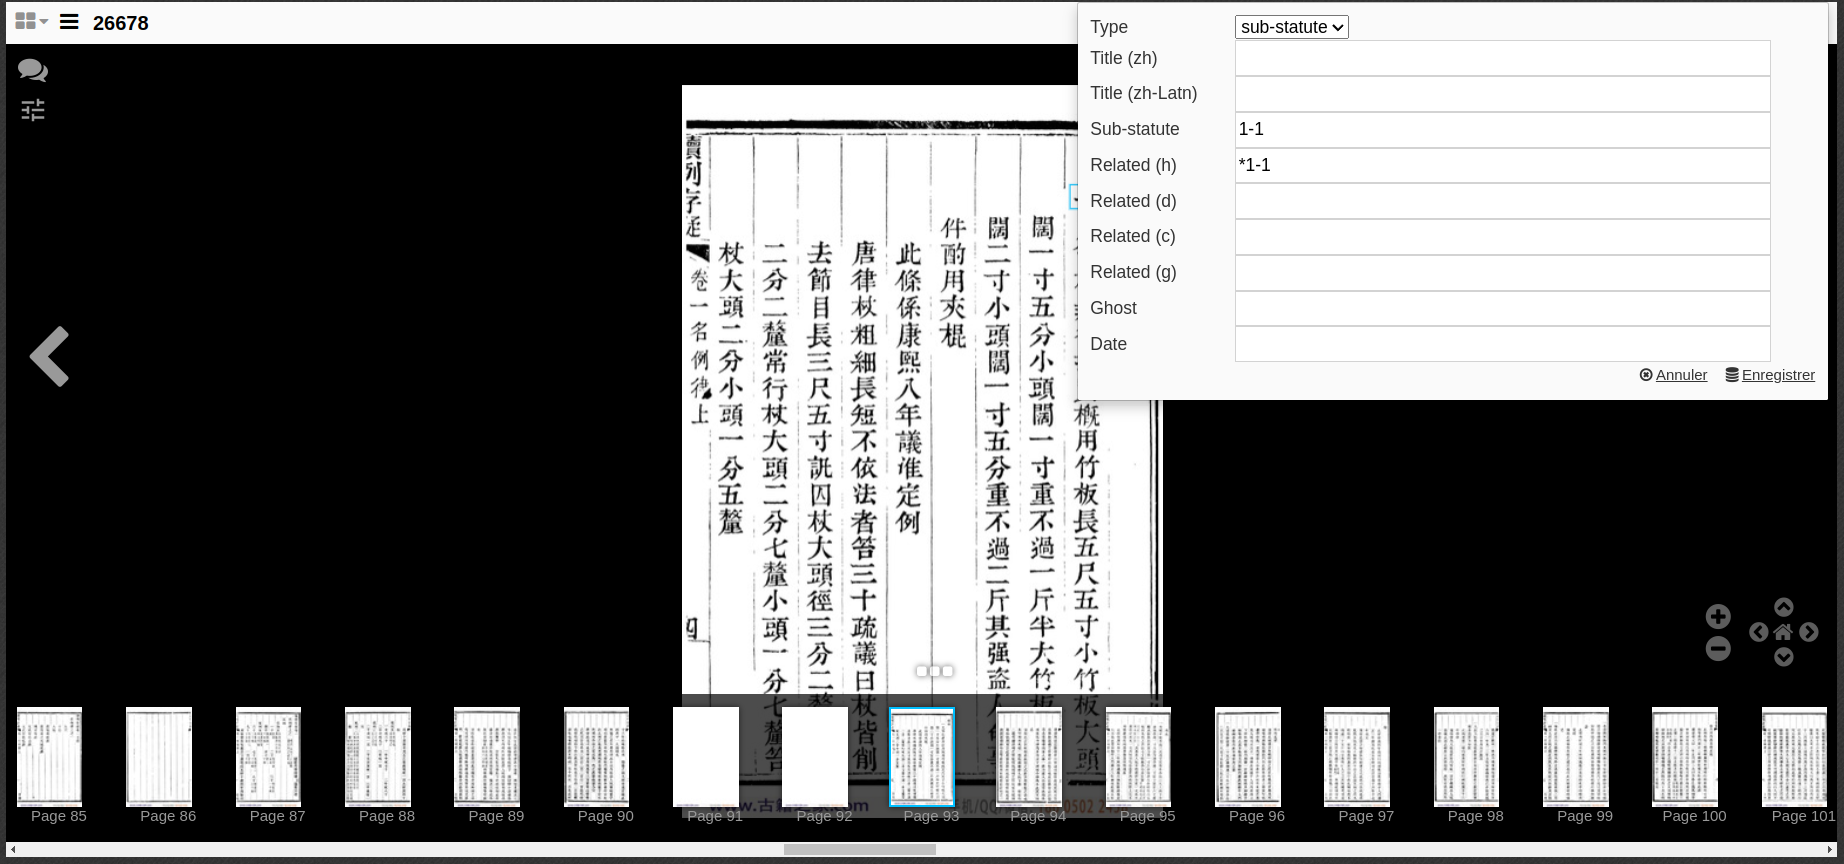
\includegraphics[width=\textwidth]{images/image3.png}
    \caption{Interface d'annotation du visualiseur Mirador}
\end{figure}
Cette pratique a permis aux chercheurs de produire des annotations structurées et uniformes d'un texte à l'autre. Dans ce cadre figurent notamment des informations sur la date de début de validité des lois et des liens de généalogie. 

\newpage
\subsubsection{Généalogie des lois}
Ce travail d'annotation et de segmentation des textes, toujours en cours en parallèle du projet \COREL, a pour objectif de retracer la généalogie des lois. Les annotations sont remplies à partir d'un référentiel. Ce référentiel prend comme source de départ le \genyuan. C'est un fichier texte disponible en ligne, hébergé par Data Futures. Il recense chaque loi une à une, généralement avec le lien vers la numérisation correspondante, et indique deux types de liens. Le premier est un lien d'association simple. Il indique les correspondances entre la loi du \genyuan à une loi d'un autre document. 
\begin{figure}[h]
    \centering
    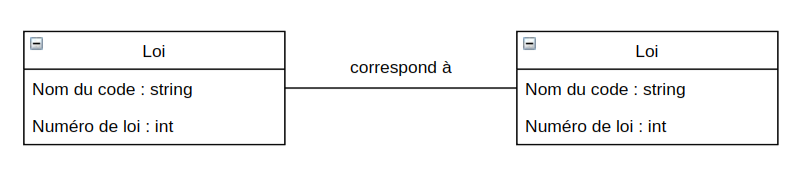
\includegraphics[width=\textwidth]{images/image4.png}
    \caption{Modélisation d'un lien d'association entre deux lois}
    \label{Modélisation d'un lien d'association entre les lois}
\end{figure}

Ce lien d'association simple est à indiquer dans les rangs \textit{related} des annotations. Elles indiquent les lois associées à celle de l'image dans les autres textes de lois, chaque lettre correspondant à une source textuelle différente : h pour \huidian, g pour \genyuan, d pour \dc et c pour \dq. 

Le référentiel indique également un deuxième type de lien, qui n'est pas présent dans les annotations des images. C'est un lien d'association dirigée, qui indique des liens de généalogie entre les lois. Pour distinguer ces liens de généalogie des liens d'association simple, les chercheurs ont mis en place dans le référentiel un vocabulaire spécifique à ces liens. Les liens \og \textit{in} \fg indiquent qu'une loi est issue d'une autre, et les liens \og \textit{out} \fg indiquent qu'une loi donne naissance à une autre.

\begin{figure}[h]
    \centering
    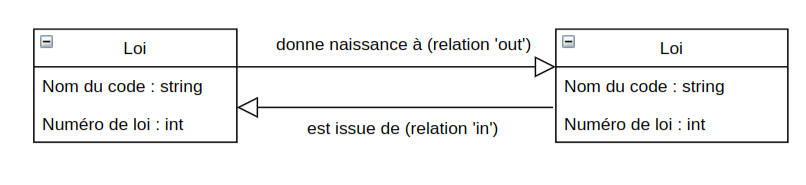
\includegraphics[width=\textwidth]{images/image5.png}
    \caption{Modélisation des liens d'association dirigée entre deux lois}
\end{figure}

Lorsque les informations du référentiel sont retranscrites dans les annotations, elles sont stockées dans des fichiers \JSON que le prestataire fournit à l'équipe du projet. Toutefois, ces données ne sont que partiellement accessible car le projet dispose uniquement des fichiers correspondant aux annotations, sans le manifeste \IIIF, ne donnant pas accès aux métadonnées, lesquelles sont accessibles uniquement via une plateforme gérée par Data Futures aux utilisateurs connectés. Cet accès se fait uniquement en interface graphique, ces données ne sont donc pas exploitables. De plus, l'annotation des images étant toujours en cours de saisie, les fichiers \JSON sont encore incomplets, puisque les valeurs ne sont pas encore entièrement saisies. Dans cet exemple, la date de début de validité de la loi n'a pas encore été saisie. 

\begin{minted}{json}
    {
            "chars" : "",
            "format" : "text/plain",
            "@type" : "freizo:date"
         },
         {
            "chars" : "254",
            "@type" : "freizo:number"
         },
\end{minted}

Ces données, en plus d'être partielles et toujours en cours de saisie, contiennent parfois des informations qui sont encore à expliciter. C'est notamment le cas du champ de date des annotations. À l'intérieur de celui-ci, les chercheurs entrent la date de début de validité d'une loi. Pour retrouver la date de fin, il est nécessaire de passer par les liens de généalogie. À partir d'un lien \textit{in}, il faut alors déduire que la date de début d'une loi B met fin à la période de validité d'une loi A. 

Les données à disposition du projet \COREL sont donc entièrement issues des deux projets précédents. Pensées et produites à des fins différentes, ces sources numériques ne sont pas liées entre elles, en plus d'être produites dans des formats différents. 

            
        \clearemptydoublepage
        
        \chapter{Traitement et structuration d'un corpus documentaire}
        Dans le cadre du projet \COREL, le stage a pour objectif de mettre en place une chaîne de traitement des données, afin de les adapter à la reconstitution de la législation de la Chine impériale tardive et de les éditorialiser.
                    \section{Le contexte de travail}
    \subsection{Une équipe issue de la collaboration inter-institutionnelle}

L'équipe du projet \COREL est composée de deux chercheurs : M. Frédéric Constant, chercheur de l'Université Côte d'Azur, responsable scientifique du projet et M. Luca Gabbiani, chercheur de l'\EFEO ; et d'un ingénieur, M. Vincent Paillusson, responsable informatique de l'\EFEO et gestionnaire à la Maison de l'Asie. La responsable administrative du projet, Mme Anne Chatellier, est la directrice des réseaux et partenariats documentaires du \cdf. Le projet s'inscrit ainsi dans un contexte de collaboration inter-institutionnelle et se trouve soumis à des contraintes à la fois géographiques, les membres de l'équipe n'étant pas réunis sur un même lieu de travail, et organisationnelles, puisque l'équipe ne travaille pas à temps plein pour le projet \COREL. 

Rattachée administrativement au \cdf lors du stage, j'ai moi-même été confrontée à ces contraintes depuis un lieu de travail différent des autres membres de l'équipe. Les échanges quotidiens du projet se déroulent majoritairement en distanciel, par mails ou visioconférences et tous les membres de l'équipe n'ont pas toujours la possibilité de se rendre disponible. Des réunions en présentiel, au \cdf ou à l'\EFEO peuvent également être organisées, mais doivent être programmées jusque plusieurs semaines en amont afin d'anticiper les obligations professionnelles de chacun. L'organisation de ces réunions aboutit généralement à des réunions longues, d'une durée supérieure à deux heures, car en plus d'être motivées par un sujet précis, elles représentent des moments rares d'échanges de l'équipe au complet et permettent de problématiser ou de résoudre certaines questions qui dépassent le cadre de la réunion. De plus, les chercheurs sont fréquemment en déplacement professionnel à l'étranger, ce qui demande un niveau d'adaptation supplémentaire : il est nécessaire d'anticiper, en plus des contraintes professionnelles, le décalage horaire. Ces contraintes d'organisation sont exigeantes pour l'équipe et leur demandent parfois de prolonger leurs journées de travail au-delà de leurs horaires habituels, complexifiant davantage les échanges hybrides.  

\subsection{Le travail déjà amorcé}
Dès mon entrée en stage, j'ai été confrontée à ces contraintes d'organisation. J'ai dû faire preuve d'une assimilation rapide des connaissances en découvrant le domaine de l'histoire du droit chinois et comprendre rapidement l'état du projet lors des réunions organisées les premiers jours, qui ont permis de réunir l'équipe du projet mais aussi des chercheurs de ce domaine d'études. Une quantité importante d'informations m'a été donnée sur une période courte de deux jours et j'ai ensuite dû apprendre à travailler à distance avec l'équipe, avec une grande place laissée à l'autonomie.

\subsubsection{Les différentes étapes de travail}
Appréhender les différentes sources, originales ou numériques, a été une difficulté supplémentaire. Le projet dispose d'un corpus assez restreint de cinq textes de lois, mais les données numériques qui en résultent sont multiples et hétérogènes. Il a donc fallu identifier en premier lieu les différentes étapes du travail déjà effectué. Les codes légaux ont d'abord été numérisés par la bibliothèques d'études chinoises puis océrisés. Les données de l'\OCR ont ensuite été encodées en \XML et publiées sur le site \LSC. L'encodage est encore en cours et le texte de l'\OCR est en train d'être corrigé. Les numérisations des codes ont ensuite été confiées au prestataire Data Futures et téléchargées sur un serveur \IIIF. Ces images ont d'abord été segmentées puis annotées. Les annotations sont en cours de corrections et d'enrichissement. 

\subsubsection{Les besoins émergents}
La présentation qui m'a été faite du projet et du travail déjà amorcé a permis aux chercheurs d'évoquer par la même occasion les besoins du projet. 
%difficultés à appréhender les différentes sources différentes et non liées, à démêler le travail des projets précédents VS le travail du projet COREL (qui, au final, n'est qu'en phase d'élaboration ?)
%les besoins qui émergent / un projet un peu à l'arrêt : site web de l'ancien projet qui ne convient plus, le propriétaire ne répond plus, pourtant on continue d'alimenter ces données. Le schéma xml ne convient plus non plus car on veut rajouter du nouveau contenu. 
%pas de pistes pour savoir comment réaliser le projet
%difficultés à définir clairement le périmètre du projet


 \section{Un projet en phase d’initialisation}
    \subsection{Définition de la mission de stage}

§ Paragraphe 1

Idée :\\
Exemple :\\
Référence :\\
Transition :\\

§ Paragraphe 2

Idée :\\
Exemple :\\
Référence :\\
Transition :\\

§ Paragraphe 3

Idée :\\
Exemple :\\
Référence :\\
Transition :\\

\subsection{Les enjeux de la mission}

§ Paragraphe 1

Idée :\\
Exemple :\\
Référence :\\
Transition :\\

§ Paragraphe 2

Idée :\\
Exemple :\\
Référence :\\
Transition :\\

§ Paragraphe 3

Idée :\\
Exemple :\\
Référence :\\
Transition :\\


\section{Les contraintes inhérentes au projet}
    \subsection{S’inscrire dans la continuité de deux projets de recherches}

§ Paragraphe 1

Idée :\\
Exemple :\\
Référence :\\
Transition :\\

§ Paragraphe 2

Idée :\\
Exemple :\\
Référence :\\
Transition :\\

§ Paragraphe 3

Idée :\\
Exemple :\\
Référence :\\
Transition :\\

\subsection{Des données hétérogènes}

§ Paragraphe 1

Idée :\\
Exemple :\\
Référence :\\
Transition :\\

§ Paragraphe 2

Idée :\\
Exemple :\\
Référence :\\
Transition :\\

§ Paragraphe 3

Idée :\\
Exemple :\\
Référence :\\
Transition :\\

\subsection{Un projet de recherche}

§ Paragraphe 1

Idée :\\
Exemple :\\
Référence :\\
Transition :\\

§ Paragraphe 2

Idée :\\
Exemple :\\
Référence :\\
Transition :\\

§ Paragraphe 3

Idée :\\
Exemple :\\
Référence :\\
Transition :\\
            
        \clearemptydoublepage


    \part{La préparation des données à l’initialisation d’un projet, enjeux de l’encodage en XML-TEI}
        \chapter{Initialisation et démarrage du projet}
                    \section{Gestion de projet}
    \subsection{Réalisation d’un état des lieux du projet}

Afin de comprendre les sources du projet \COREL et le travail effectué lors des projets précédents, il a été nécessaire de faire un état des lieux, à intégrer dans le cahier des charges. En effet, les projets \LSC et \EPJ n'ont pas produit de documentation, ce qui rend la compréhension de ces projets difficile. Seuls les chercheurs ayant travaillé sur ces projets sont à même d'expliquer le travail effectué et les productions qui en découlent. De plus, sans connaissances préalables sur le droit chinois, les sources numériques produites ne sont pas suffisamment claires pour être instantanément comprises par un ingénieur et ne se suffisent pas à elles-mêmes, d'autant plus avec un schéma d'encodage personnalisé, qui a pu se transformer avec le temps. Dès lors, l'état des lieux des projets précédents est indispensable afin de préparer les données pour le projet \COREL, d'autant plus que l'enrichissement des données \LSC et \EPJ est toujours en cours. 



\subsection{Définir les livrables attendus du projet}

§ Paragraphe 1

Idée :\\
Exemple :\\
Référence :\\
Transition :\\

§ Paragraphe 2

Idée :\\
Exemple :\\
Référence :\\
Transition :\\

§ Paragraphe 3

Idée :\\
Exemple :\\
Référence :\\
Transition :\\

\subsection{Prioriser certains aspects du projet}

§ Paragraphe 1

Idée :\\
Exemple :\\
Référence :\\
Transition :\\

§ Paragraphe 2

Idée :\\
Exemple :\\
Référence :\\
Transition :\\

§ Paragraphe 3

Idée :\\
Exemple :\\
Référence :\\
Transition :\\

 \section{Importance de l’étape de préparation des données}
    \subsection{La diversité des données des projets précédents}

§ Paragraphe 1

Idée :\\
Exemple :\\
Référence :\\
Transition :\\

§ Paragraphe 2

Idée :\\
Exemple :\\
Référence :\\
Transition :\\

§ Paragraphe 3

Idée :\\
Exemple :\\
Référence :\\
Transition :\\

\subsection{Établissement d’un écosystème de données}

§ Paragraphe 1

Idée :\\
Exemple :\\
Référence :\\
Transition :\\

§ Paragraphe 2

Idée :\\
Exemple :\\
Référence :\\
Transition :\\

§ Paragraphe 3

Idée :\\
Exemple :\\
Référence :\\
Transition :\\

            
        \clearemptydoublepage
        
        \chapter{L’encodage en XML-TEI : un format standard des données}
                    \section{Pourquoi se conformer à un standard ? }
    \subsection{Un langage recommandé pour l’édition scientifique numérique}

Les corpus encodés en \TEI sont de plus en plus nombreux dans les projets de recherche en humanités numériques. La \TEI permet de préconiser des standards d'encodage au format \XML. Ces préconisations sont documentées dans les \textit{guidelines} disponibles en ligne et permettent d'assurer l'interopérabilité des données encodées en \XML pour l'édition scientifique numérique, en privilégiant un encodage sémantique afin de décrire les documents. Ce standard permet de s'adapter à un grand nombre de documents, nativement numériques ou transpositions de sources matérielles, et offre donc de nombreuses possibilités d'encodage et un niveau de personnalisation élevé, ce qui explique son utilisation de plus en plus majoritaire dans les projets d'édition scientifique numérique.

\begin{quote}
    La TEI met l’accent sur ce qui est partagé par tous les types de documents, qu’ils soient représentés physiquement sous une forme numérique sur un disque ou une carte mémoire, sous une forme imprimée comme un livre ou un journal, sous une forme écrite comme un manuscrit ou un codex, ou sous une forme inscrite dans la pierre ou sur une tablette de cire. Cette continuité facilite la migration du texte depuis des manifestations plus anciennes, comme l’imprimé ou le manuscrit, vers d’autres plus récentes comme le disque ou l’écran. \footnote{\cite{burnard_tei_2015}}
\end{quote}

En s'adaptant à tous types de documents, la \TEI représente un format de données idéal pour le projet \COREL : les textes de lois étant produits selon une architecture définie et régulière, ils se prêtent particulièrement bien à un encodage sémantique, qui permet de mettre en avant les éléments structurants des textes. De plus, la \TEI offre un vaste choix de balises, ce qui permet aux chercheurs du projets de pouvoir enrichir leurs sources, conformément aux objectifs du projet. Encoder les documents en \TEI garantit à la fois un encodage régulier et cohérent grâce à sa documentation, flexible et bien adapté aux sources grâce aux nombreuses possibilités d'encodage. Le passage à des documents encodés en \TEI, en plus de contribuer à l'interopérabilité des données de la recherche, assure aux chercheurs une indépendance dans les choix éditoriaux, contrairement au schéma figé du projet \LSC utilisé jusqu'à présent. Malgré la richesse de la \TEI, il est possible que l'utilisation de certains éléments ne correspondent pas entièrement aux spécificités d'un texte. Toutefois, ce cas de figure est également prévu par la \TEI. Il est en effet possible d'étendre le standard en modifiant le schéma d'encodage dans l'\ODD. Deux types de modifications de la \TEI sont alors possibles : des modifications dites \TEI \textit{conformant}, qui respectent les règles de la \TEI, ou bien des modifications qui outrepassent ces règles, bien que ces dernières ne soient pas conseillées. Que la \TEI soit étendue ou non, il est essentiel d'avoir un projet bien documenté, qui permette à d'autres utilisateurs de la \TEI de comprendre comment les données ont été structurées et quels choix d'encodage ont été faits. 

\subsection{Interopérabilité et documentation en ligne}

La \TEI a été créée en 1987 pour promouvoir un standard d'encodage des données en humanités numériques et ainsi permettre l'interopérabilité des ressources en ligne. En effet, le numérique apporte un foisonnement de données et de formats divers et souvent incompatibles entre eux, qui rendent l'échange des données difficile, voire impossible. Établir un standard de la diffusion des données en \textit{open access} afin de garantir leur accessibilité devient un enjeu majeur corrélé à l'apparition du web et à l'essor des formats propriétaires au profit des entreprises privées. Bien que les principes de science ouverte continuent de se développer aujourd'hui, il est primordial de maintenir la conformité à des standards afin de produire des données \fair et pérennes. 

Le principe \fair des données est l'un des enjeux du projet \COREL. En effet, les chercheurs ont été sensibilisés à l'importance de l'ouverture des données via le projet \LSC, qui présente de nombreuses contraintes résultant du manque d'\textit{open access}. Les données \XML n'étant pas libre d'accès ni interopérables, et le site internet propriétaire ne répondant plus aux besoins d'évolution du projet, contribuer à la science ouverte et faciliter l'accès aux sources (les textes de lois mais aussi leur transposition en sources numériques) est primordial afin d'enrichir les sources du droit chinois dans le domaine du numérique. 

L'encodage des données en \TEI permet de produire des données interopérables et réutilisables par la communauté de chercheurs en sciences humaines, selon les recommandations du \wc. C'est également un avantage pour l'équipe du projet, qui peut se référer aux \textit{guidelines} et accéder à une documentation claire et fournie, ce qui permet de faire des choix d'encodage adaptés et d'obtenir des documents \TEI valides. Cela permet aussi de se nourrir d'autres projets de recherche qui utilisent la \TEI et de pouvoir accéder à des outils de publication de données comme \tp. En effet, de nombreux exemples de données encodées en \TEI et publiées avec \tp sont disponibles en ligne. Dans le cadre du projet \COREL, deux exemples ont notamment été étudiés : le projet \disco de l'INRIA, qui présente des éditions scientifiques numériques de correspondances et le projet \cordel de l'Université de Genève. Ces deux exemples permettent d'illustrer l'adaptabilité du langage \TEI, qui permet d'encoder des documents très différents : des correspondances, de la littérature de colportage ou, dans le cas du projet \COREL, des textes de lois. 

 \section{La transformation en XML-TEI}
    \subsection{Une transformation adaptée aux besoins du projet}
    
En plus de pouvoir s'appuyer sur des exemples de projets de recherche, encoder les documents du corpus en \TEI a permis d'établir un schéma d'encodage stable. En effet, les balises \TEI sont documentées dans les \textit{guidelines} et ont une utilisation prédéfinie, ce qui permet d'assurer la régularité de l'encodage au fur et à mesure du projet. Contrairement au schéma \LSC qui proposait une petite quantité de balises dont l'usage initial à été détourné au fil du temps, comme par exemple les balises \texttt{<content>}, un encodage en \TEI diminue le risque de mésusage des balises grâce à sa documentation. De plus, l'encodage du projet a pu s'écarter d'un schéma pensé pour l'affichage du texte afin d'adopter l'orientation sémantique de la \TEI. À court termes, cette pratique d'encodage offre une meilleure compréhension et structuration des documents, qui n'est plus liée à son affichage \HTML. À long termes, un encodage sémantique permet de produire un jeu de données qui pourra être réutilisé par les chercheurs. 

Il est pertinent de considérer les données comme un matériau à partir duquel le projet produit des livrables : si certains chercheurs en histoire du droit chinois consulteront le produit fini que sera le site web du projet, d'autres, initiés aux humanités numériques, pourront également consulter les données \TEI et les prendre comme support pour leurs propres recherches. Dissocier les données des livrables permet aussi d'enrichir les données de la recherche, puisque le projet \LSC notamment n'offre pas de données en libre-accès mais simplement les résultats produits à partir de ces données. Cette pratique d'un encodage sémantique, interopérable vient donc répondre à l'une des problématiques principales du projet au début du stage : la réutilisation de données produites pour un projet spécifique, qui ne respectent pas les principes \fair des données puisqu'elles ne sont pas disponibles en ligne librement (l'accès au site web \LSC est possible, mais les données ne sont pas mises à la disposition des chercheurs), non-interopérables car malgré le format d'encodage \XML, le schéma est entièrement personnalisé et non-documenté, ce qui aboutit enfin à des données qui peuvent difficilement être réutilisées. Le projet \COREL, en transformant ces données en \TEI, contribue ainsi à la science ouverte et à l'enrichissement des données de la recherche, tout en bénéficiant d'un encodage mieux adapté aux besoins du projet. 

\subsection{La transformation XSLT}

Le projet \cordel est l'un des exemples sur lequel le projet \COREL prend appui. Les données des deux projets présentent en effet des similarités. Issues de l'\OCR, les données ont d'abord été encodées en \XML. Pour le projet \COREL, cet encodage provient d'un projet antérieur, tandis que pour le projet \cordel, les données de l'\OCR ont été encodées automatiquement par \textit{Transkribus}. À l'instar de l'Université de Genève, les données des codes légaux chinois ont ensuite été transformées via le langage \XSLT en documents \TEI valides. 

Le langage \XSLT est un langage \XML conçu pour transformer des documents \XML en documents \XML, \HTML ou \LaTeX. Un document \XML en entrée passe par un processeur \XSLT avec des instructions \XSL rédigées dans une feuille de style.

\begin{figure}
    \centering
    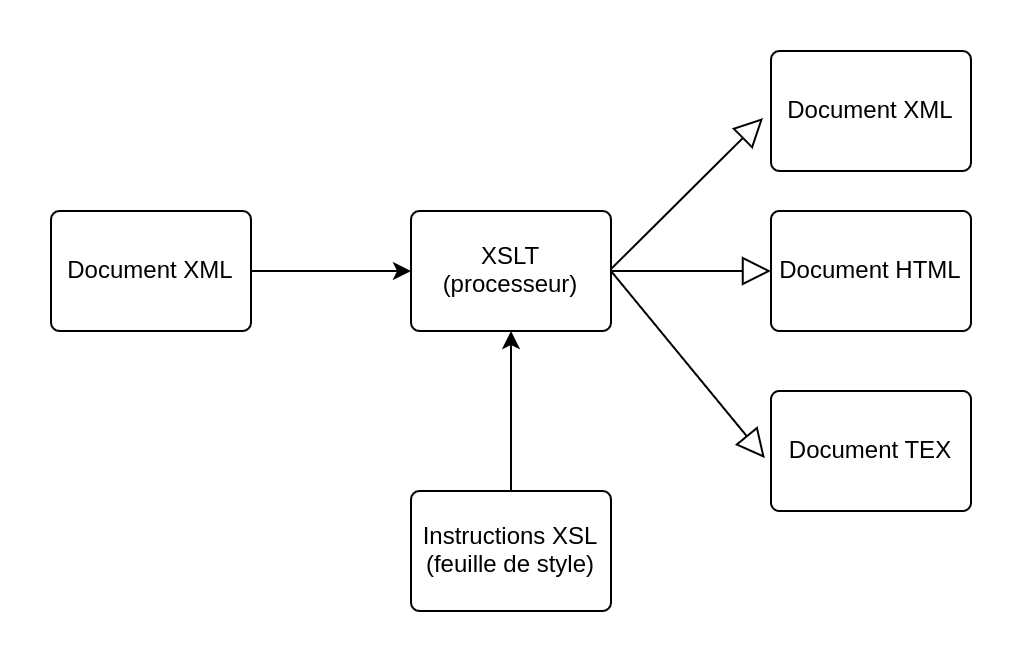
\includegraphics[width=\textwidth]{images/xslt.png}
    \caption{Modélisation de la transformation \XSLT}
\end{figure}

Les données du projet \LSC conservent la structure générale des codes légaux chinois. Cela facilite la transformation \XSLT qui maintient cette structure en chapitres, sections et lois en sélectionnant uniquement les éléments structurants. Toutefois, l'une des difficultés de cette transformation, malgré la structure rigoureuse des textes chinois, découle de la modification des pratiques d'encodage dans le temps. En effet, puisque certaines balises sont utilisées selon des usages différents d'un document à l'autre, il est nécessaire de penser les règles de transformation avec de nombreuses exceptions. Ces contraintes ont donné lieu, dans un premier temps, à un code verbeux à l'intérieur duquel de nombreuses conditions \texttt{<xsl:if>} et \texttt{<xsl:when>} étaient imbriquées. Le code, en plus d'être difficile à lire, risquait de plus d'aboutir à des erreurs sur certaines de ces exceptions, erreurs difficilement repérables puisque je ne suis pas en mesure de lire les documents chinois. 

Dans ces circonstances, il est essentiel d'écrire un code qui soit le plus clair et simple possible, pour aboutir à un risque d'erreur faible. Les nombreuses conditions imbriquées les unes dans les autres, en plus d'être compliquées à lire et de présenter un risque d'erreur important si l'une des conditions n'est pas remplie, peut également complexifier les chemins \xpath à renseigner dans les règles de transformation puisque le \xpath tient compte de ces imbrications : il faut ainsi toujours tenir compte du noeud courant spécifié dans la règle parente. 

\begin{minted}{xslt}
     <xsl:for-each select="./li">
        <div type="substatute">
            <xsl:attribute name="n">
                <xsl:value-of select="./@id"/>
            </xsl:attribute>
            <pb/>
            <xsl:for-each select="./content[@lang='ch']">
                <p>
                    <xsl:apply-templates/>
                </p>
            </xsl:for-each>
        </div>
    </xsl:for-each>
\end{minted}

Dans cet exemple simple d'une règle pour reproduire les \li dans un élément \texttt{<div>}, trois chemins \xpath sont nécessaires : le premier sélectionne toutes les balises \texttt{<li>} du document \XML, et les deux autres sélectionnent des éléments ou attributs à partir du noeud courant, c'est-à-dire contenus à l'intérieur de la balise \texttt{<li>}. De plus, les \li sont des articles additionnels, qui sont donc contenus dans des éléments parents (les \lu). Il est ainsi possible d'observer qu'une règle simple, sans conditions particulières, requiert déjà une attention accrue portée au \xpath. Utiliser des règles imbriquées trop profondément les unes dans les autres pour transformer des documents que je suis incapable de lire n'était donc pas la solution idéale pour traiter les données. Écrire des règles complexes afin de prendre en compte les spécificités de chaque document, que leur lecture soit possible ou non, n'est d'ailleurs pas une solution adaptée au traitement d'un grand nombre de données. En effet, un code trop complexe et difficile à corriger risque de produire des erreurs qui ne seront pas repérées à la vérification, car il n'est pas envisageable de relire tous les documents un à un. 

Toutefois, le corpus étant composé d'un petit nombre de documents, une granularité fine de la feuille de style est envisageable, c'est pourquoi les règles de transformations ont été divisées en plusieurs éléments \texttt{<xsl:template>} : un template pour rédiger le \texttt{<teiHeader>} commun à tout le corpus puis un template pour chaque document du corpus. 

\begin{minted}{xslt}
    <!-- Nouveau template pour le code de 1740 -->
    <xsl:template match="/code[@id='DQLL1740']/document">
    ...
    </xsl:template>

    <!-- Nouveau template pour le code de 1646 -->
    <xsl:template match="/code[@id='code1646']/document">
    ...
    </xsl:template>
\end{minted}
Dans les sources numériques du projet \LSC, chaque document a un identifiant unique, ce qui permet de faire un template par code légal, tout en ayant des templates généraux comme pour le \texttt{<teiHeader>}. Rédiger un template pour chaque document peut sembler redondant puisque la structure globale des textes de lois reste la même (chaque template présente une règle sur les chapitres, les sections, les \lu et les \li). Toutefois, des variations dans l'encodage sont difficile à prendre en compte dans un seul template : notamment l'usage de la balise \texttt{<content>} comme vu précédemment, mais aussi des variations entre les codes légaux et les compilations. Le \huidian par exemple présente du contenu supplémentaire, encodé dans des balises \texttt{<part>}, qui contiennent des listes de lois. Pour prendre en compte ces exceptions, l'utilisation de plusieurs templates permet de rendre le code plus lisible et moins verbeux. De plus, les données \LSC continuant d'être enrichies en parallèle du projet \COREL, la feuille de style n'est pas un outil à usage unique et est amenée à être modifiée par d'autres, ce qui renforce l'intérêt de produire un code clair et compréhensible. 

Si la structure des textes n'a pas été modifiée, la transformation vers la \TEI a toutefois permis d'apporter des modifications et de sémantiser le balisage \XML. Les sources originales présentent la numérotation des chapitres, sections et lois dans un attribut \texttt{@id}. Toutefois, cette solution ne répondait pas pleinement aux spécificités des codes légaux, puisque ces chiffres représentent une numérotation des lois et chapitres plutôt qu'un identifiant unique. En effet, deux lois avec le même \texttt{@id} d'un texte de loi à un autre ne sont pas nécessairement liées entre elles, puisque chaque document suit une numérotation continue, sans lien avec les autres sources. Cet attribut \texttt{@id} a donc été resémantisé via l'attribut \texttt{@n} afin de laisser place à des identifiants uniques, les attributs \texttt{@xml:id}, pour lier les lois entre les différents codes. Cette resémantisation des attributs permet une meilleure compréhension de la structure des documents : les lois sont liées entre elles, mais la numérotation peut différer d'un texte à un autre.

Des attributs \texttt{@type} ont également été ajoutés sur de nombreux éléments, afin de les spécifier et de les adapter aux documents du corpus. Ainsi, tous les éléments structurants des textes de lois ont été transformées en éléments \TEI \texttt{<div>}. Ce choix d'encodage permet de mettre en avant la structure du document, mais nécessite l'ajout d'un attribut afin de préciser le type de cet élément. Dans l'encodage \LSC, les quatre éléments principaux sont \texttt{<bu>, <men>, <lu>, <li>}. La transformation \XSLT permet de structurer l'information donnée par ces balises : ce sont d'abord des éléments structurants des documents (des éléments \texttt{<div>}), mais aussi sémantiques : des attributs \texttt{@type='chapter | section | statute | substatute'} ont donc été ajoutés. Cette structuration de l'information permet à des chercheurs non-spécialistes de comprendre la structure des sources. De plus, le site web du projet \COREL s'adresse à des chercheurs en droit chinois en France autant qu'à l'étranger, c'est pourquoi des noms d'attributs anglais sont adaptés au public cible.

La transformation \XSLT a ainsi permis de modifier les sources \XML afin de produire un jeu de données réutilisable et facilement accessible par les chercheurs. L'encodage en \TEI a permis de restructurer les informations présentes dans l'encodage et de mieux sémantiser les éléments pour une meilleur appréhension des documents. Cette transformation s'inscrit, de plus, dans une démarche de contribution à la science ouverte et à l'enrichissement des données de la recherche.

             
            
        \clearemptydoublepage
        
        \chapter{Définir le modèle de données du projet}
                    \section{Établir un modèle de données}
    \subsection{Réalisation d'un échantillon des données}

La préparation des données du projet \COREL s'effectue en coopération avec le prestataire. En effet, la société Data Futures est le gestionnaire de la plateforme d'annotation dans laquelle les chercheurs saisissent les données manquantes pour le projet, notamment les dates de début de période d'application des lois et les liens d'association et/ou d'association dirigée entre les lois. Ces informations sont présentes dans les annotations mais ont besoin d'être explicitées afin de pouvoir être ajoutées dans l'encodage : il est nécessaire d'ajouter des dates de fin d'application des lois notamment. L'équipe du projet a donc fait appel au prestataire afin de générer automatiquement les dates de fin de validité des lois à partir des liens de généalogie. Lorsqu'une loi en remplace une autre, la date de promulgation de la nouvelle loi marque la fin de l'application de la précédente. La chaîne de traitement des données est donc la suivante : les chercheurs enrichissent les données des annotations et les corrigent ; le prestataire génère automatiquement les dates de fin de validité des lois pour obtenir des bornes chronologiques ; les données sont ajoutées à l'encodage \TEI. Lors du stage, la première étape de cette chaîne de traitement était en cours de réalisation. La deuxième étape, prévue dans le calendrier du projet, indique que le prestataire fournit les données via des fichiers \JSON au mois de septembre. 

Afin d'anticiper la dernière étape de préparation des données, un échantillon des données a été réalisé sur un extrait du \dc, chapitre 6, section 25, \lu 254 et \li 1. Cet échantillon permet d'encoder les données manquantes afin d'établir le modèle d'encodage qui sera utilisé pour ajouter les données \JSON en \TEI. Dans un premier temps, il a été nécessaire d'identifier tous les types de données à ajouter et de déterminer les éléments \TEI les plus pertinents pour encoder ces informations. Cette étape a été réalisée une fois les documents \XML transformés en \TEI. Pour mener à bien le projet, il est pertinent d'ajouter dans l'encodage : 
\begin{itemize}
    \item Les bornes chronologiques pour chaque \lu et \li.
    \item Le lien vers les numérisations des textes.
    %à vérifier : est-ce que j'ai parlé au début du fait qu'on veut inclure les numérisations dans le site web, dans un visualiseur 3IF ?? mais que les ressources ne sont pas accessibles en ligne et que on ne peut pas accéder aux manifestes ? (et que l'équipe du projet ne le souhaite pas ?????)
    \item Un identifiant unique pour chaque \lu et \li permettant d'identifier dans chaque texte les lois associées.
    \item Des commentaires supplémentaires (de nature différente des commentaires officiels).
    \item L'enrichissement des données sur les entités nommées.
\end{itemize}

Ces éléments ont été choisis conjointement avec les chercheurs afin d'obtenir en résultat une édition en ligne complète et exploitable pour les chercheurs. À partir de cette liste, un modèle d'encodage à suivre a pu être mis en place. 

\begin{minted}{xml}
    <div type="substatute" n="1" xml:id="DQLL_254_1" 
         notBefore="1833" notAfter="1870">
        <pb  
        facs="https://duli-cunyi.freizo.org/mirador/book.cgi?catno=28941&amp;
        canvas=https://iiif.duli-cunyi.freizo.org/image/28941/canvas/p5"/>
            <p>一、反逆案内律應問擬凌遲之犯,其子孫訊明,
            實係不知謀逆情事者,無論已未成丁,均解交内務府閹割,發往新疆等處,
            給官兵為奴。如年在十歲以下者,牢固監禁,俟年届十一歲時,再行解交内務府,
            照例辦理。内務府大臣遇有解到閹割人犯,即遴派司員認眞看驗,並出具無弊切結,
            送交刑部,再行覆驗。如有情弊,即行奏參,務須查驗明確,再交兵部,發往新疆,
            給官兵為奴。至其餘律應緣坐男犯,並非逆犯子孫,年在十六歲以上者,
            發往新疆等處,給官兵為奴。如年在十五歲以下者,牢固監禁,
            俟成丁時再行發遣。緣坐婦女,發各省駐防,給官員兵丁為奴。
            其知情不首干連人犯,仍依律擬流。</p>
            <note type='metadata'>Notes on the law</note>
    </div>
\end{minted}

\subsubsection{Liens vers les images}
Les liens vers les images peuvent être ajoutés via l'attribut \texttt{@facs} sur les balises \texttt{<pb/>} qui indiquent le début d'une nouvelle page. Ces balises ont été ajoutées aux sources numériques afin de faciliter la pagination de l'édition numérique et permettra d'afficher l'image en regard du texte. Le projet \COREL souhaite aboutir à une éditon simple qui propose le texte et l'image correspondante à la page près. Un facsimile interactif n'est pas envisagé, c'est pourquoi seul l'attribut \texttt{@facs} a été choisi pour intégrer les images à l'encodage. Cette solution a également été adoptée pour le projet \cordel : 
\begin{minted}{xml}
     <div>
        <pb n="1" source="Moreno_001_1.jpg" 
        facs="fedora_ug8110021/full/full/0/default.jpg"/>
        ...
    </div>
\end{minted}

L'intégration des images pose toutefois un problème d'\textit{open access} qui n'a pas pu être résolu dans le cadre de mon stage. En effet, l'équipe du projet ne dispose pas des liens \IIIF des images, contrairement au projet \cordel. Une \URL \IIIF accepte plusieurs paramètres qui permettent d'afficher différentes zones de l'image à partir des pixels. Dans l'exemple du projet \cordel, l'image est affichée en entier grâce au paramètre \texttt{full}. Les liens \IIIF des numérisations des codes légaux, de même que les liens des ressources images seules (indiquées dans les fichiers \JSON en tant qu'identifiant), ne sont pas disponibles sur le web. Le prestataire ne fournit que le lien permettant d'accéder à l'image via leur serveur. Cela pose un problème d'accessibilité, en cours de résolution par l'équipe du projet, afin que les numérisations soient librement accessibles sur le web et que les liens puissent être inclus dans l'édition numérique. Dans l'échantillon, il a été décidé d'inclure le lien présent dans les fichiers \JSON, bien qu'il ne soit pas accessible pour le moment. Une fois l'accès autorisé par le prestataire, utiliser les liens des fichiers \JSON permettra d'automatiser l'ajout des liens dans l'encodage via un script. Cette solution est la plus satisfaisante pour le projet, étant donné que la majorité des informations à ajouter doivent l'être depuis les fichiers \JSON. \footnote{Ressource image issue de l'article \og C'est quoi le IIIF ? \fg de l'Université de Genève.}

\begin{figure}
    \centering
    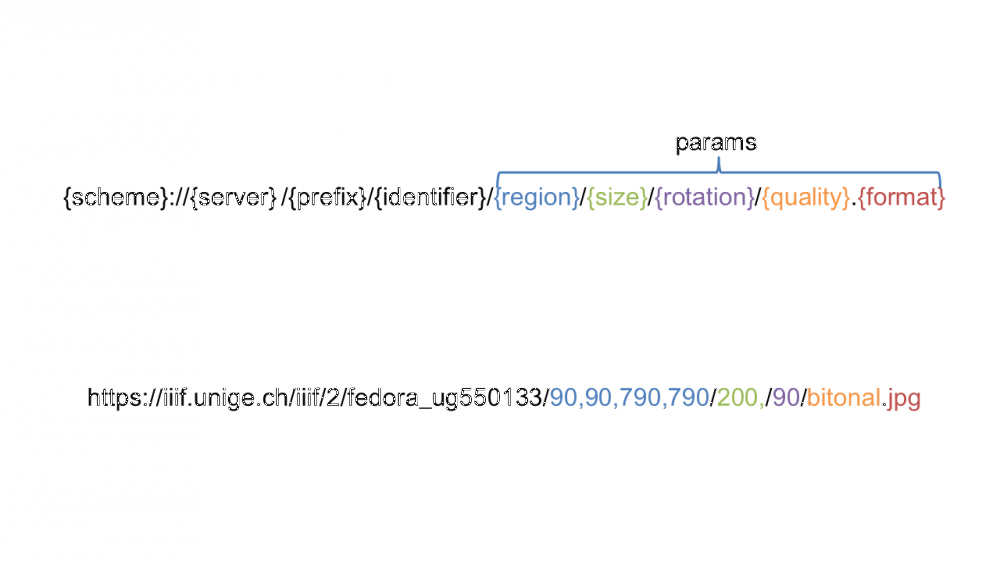
\includegraphics[width=\textwidth]{images/iiif.png}
    \caption{Schéma explicatif d'une \URL \IIIF}
\end{figure}
 
\subsubsection{Les bornes chronologiques et les identifiants \XML}
L'ajout des bornes chronologiques est également permis par des attributs \TEI. Sur chaque \lu et \li, contenues dans des éléments \texttt{<div/>}, il est possible d'ajouter des attributs \texttt{@notBefore} et \texttt{@notAfter} afin d'ajouter les dates à l'encodage. Toutefois, cet ajout demande un élargissement des règles de la \TEI car ces attributs ne sont pas autorisés sur des éléments \texttt{<div/>}. L'ajout de ces attributs est indispensable afin de reconstituer la législation pour une année donnée. Placer ces attributs sur les balises \texttt{<div/>} est nécessaire afin de pouvoir afficher la loi contenue dans cette balise afin de créer le \cv, c'est pourquoi la modification de la \TEI a été choisie pour cet élément. En plus de ces bornes chronologiques, l'élément \texttt{<div/>} contient l'attribut \texttt{@xml:id} qui permet d'attribuer à chaque loi un identifiant unique. Cela permet de faire le lien avec les fichiers \JSON et d'attribuer aux lois associées, c'est-à-dire les lois qui sont les mêmes d'un texte à un autre, le même identifiant. 

Les données à inclure dans les attributs font le lien entre le format \XML et le format \JSON. Toutefois, d'autres informations d'enrichissement des données doivent être ajoutées. 

\subsubsection{Les commentaires et les entités nommées}
Les commentaires et les entités nommées sont des informations additionnelles, qui ne sont pas présentes dans les annotations. En effet, les commentaires ont été océrisés mais n'ont pas été ajoutés dans l'encodage \XML du projet \LSC, ni dans les annotations. Quelques informations sur les entités nommées ont été ajoutées dans les annotations, toutefois elles restent partielles et n'ont pas été corrigées. 

Plusieurs types de commentaires existent dans les textes de lois chinois. Les commentaires officiels, rédigés en même temps que le texte de loi, sont déjà présents dans l'encodage dans des éléments \texttt{<note type='official'/>}. Ils apparaissent dans les sources originales dans une police de caractère légèrement inférieure. Sur le site web \LSC, l'affichage met en valeur ces commentaires avec une couleur différente du reste du texte. D'autres commentaires, notamment d'auteurs ayant rédigés les compilations, seront ajoutés à l'édition en ligne. Elles sont représentées dans l'échantillon par des balises \texttt{<note/>}, toutefois leur type n'a pas encore été défini. À des fins explicatives, un attribut \texttt{@type} a été ajoutés sur ces balises pour indiquer que chaque commentaire doit posséder cet attribut obligatoire, avec un type défini.

De plus, des commentaires qui ne sont pas présents dans l'\OCR peuvent également être ajoutés, afin de créer dans l'édition en ligne un mode \og métadonnées \fg qui permettrait d'afficher des informations supplémentaires sur les lois. Ces commentaires ont donc un attribut \texttt{@type='metadata'}. 

Par ailleurs, l'équipe du projet souhaite également enrichir les informations sur les entités nommées, afin d'envisager dans l'édition en ligne un mode \og entités nommées \fg pour les mettre en avant. Dans l'encodage \LSC, les entités nommées sont balisées par des éléments \texttt{<personname/>} ou \texttt{<propername/>}. Le projet \COREL souhaite encoder un peu plus précisément les noms de personnes en leur ajoutant notamment un nom de rôle : 

\begin{minted}{xml}
    <persName role="governor" ref="#覺羅伍拉納">
        <roleName>福建巡撫</roleName>
        <name>覺羅伍拉納</name>
    </persName>
\end{minted}
En effet, la plupart des personnes mentionnées sont des fonctionnaires et ont donc un rôle qui peut être mis en valeur dans l'encodage. Afin d'éviter les erreurs d'encodage et de garantir sa régularité, il est pertinent d'ajouter dans le \texttt{<teiHeader/>} les informations relatives à ces entités nommées dans un élément \texttt{<listPerson/>} : 

\begin{minted}{xml}
     <listPerson>
        <person xml:id="覺羅伍拉納">
            <persName role="governor" ref="#覺羅伍拉納">
                <roleName>福建巡撫</roleName>
                <name>覺羅伍拉納</name>
            </persName>
            <note>Biographical information</note>
        </person>
        <person xml:id="何東山">
            <persName role="party" ref="#何東山">
                     何東山
            </persName>
            <note>Biographical information</note>
        </person>
        <person xml:id="何適">
            <persName role="party" ref="#何適">
                     何適
            </persName>
            <note>Biographical information</note>
        </person>
    </listPerson>
\end{minted}
Lister les entités nommées dans le \texttt{<teiHeader/>} permet de les identifier grâce à un attribut \textit{@xml:id} et donc d'afficher les informations relatives à chaque entité nommée si un mode \og entités nommées \fg est créé pour le site web. Le lien entre l'identifiant \XML et le nom de personne dans l'encodage s'effectue grâce à l'attribut \texttt{@ref}. Le modèle d'encodage des entités nommées a pu être déterminé grâce à l'exemple du projet \disco de l'INRIA. En effet, leur projet accorde une place importante aux entités nommées puisqu'ils offrent une édition numérique de correspondances : 
\begin{minted}{xml}
     <listPerson>
        <person xml:id="p0001">
            <persName>d'Estournelles de Constant, Paul</persName>
            <persName>
                <roleName type="nobility">Baron</roleName>
                <forename>Paul</forename>
                <nameLink>d'</nameLink>
                <surname>Estournelles de Constant</surname>
            </persName>
            <persName>Paul Henri Balluet d'Estournelles de Constant</persName>
            <nationality>French</nationality>
            <birth>
                <date when-iso="1852-11-22"/>
                <placeName>La Flèche (Sarthe)</placeName>
            </birth>
            ...
        </person>
    </listPerson>
\end{minted}
L'édition en ligne de \disco offre un encodage exhaustif des entités nommées, dans un fichier d'index \TEI dédié à cet usage. Dans le cadre du projet \COREL, un fichier d'index n'est pas envisagé pour le moment étant donné que le corpus est constitué d'un nombre restreint de documents et que les entités nommées ne sont pas le centre du projet. Toutefois, la liste des entités nommées pourra être transposée dans un index si l'encodage s'enrichit et donne lieu à une liste et à des informations exhaustives. Pour ajouter des informations additionnelles pour chaque entité nommée, l'échantillon propose une balise \texttt{<note/>} pour ajouter des informations biographiques, sans structure prédéfinie, qui pourront être affichées dans le mode \og entités nommées \fg. 

Pour le balisage des noms de lieux, une structure similaire a été mise en place dans l'échantillon. Une liste des lieux est présente dans le \texttt{<teiHeader/>} : 
\begin{minted}{xml}
     <listPlace>
        <place xml:id="寧古塔">
            <placeName ref="#寧古塔">
                寧古塔
            </placeName>
            <note>Information about the place</note>
        </place>
    </listPlace>
\end{minted}
À l'instar des noms de personnes, le nom du lieu possède un identifiant unique qui permet de le lier au balisage présent au sein du texte et un élément \texttt{<note/>} afin d'ajouter des informations supplémentaires sur le lieu. Les noms de lieux sont mentionnés dans les textes de loi en tant que lieu d'où provient l'origine de la loi ou bien en tant que lieu d'application. Selon le contexte, la balise \texttt{<placeName/>} porte donc l'attribut \texttt{@type} avec pour valeur \texttt{'application'} ou \texttt{'origin'}. 

L'établissement d'un échantillon des données permet ainsi de fournir un modèle d'encodage à suivre pour la suite du projet et donne un aperçu de l'état final du jeu de données \TEI. L'exercice a pu mettre en valeur les difficultés qui peuvent être rencontrées lors de l'encodage, notamment l'accessibilité des ressources ou le besoin d'étendre la \TEI, et ainsi de les anticiper et de commencer à les résoudre en amont afin de pouvoir enrichir le jeu de données dès le mois de septembre. Toutefois, il est également pertinent d'étudier les limites de cet aperçu idéalisé des données.

\subsection{Limites de cet aperçu idéalisé des données}
L'échantillon de données offre un modèle de données à suivre afin de réaliser le projet. Toutefois, il représente un aperçu idéalisé des données telles que l'équipe du projet les envisage à la fin du financement, afin d'offrir aux chercheurs une édition scientifique numérique la plus complète possible. Les contraintes de temps et de financement peuvent influer sur ce modèle de données et son niveau de complétude. L'échantillon permet alors de mettre en lumière les informations manquantes dans l'encodage à un instant T, notamment les informations qui seront essentiels pour mener à bien le projet (les bornes chronologiques et les identifiants \XML). Cet aperçu idéalisé des données peut être réalisé dans le périmètre du projet en automatisant l'encodage via des scripts : les données à ajouter depuis les fichiers \JSON pourront être ajoutées automatiquement. Cependant, le balisage des entités nommées et l'ajout des commentaires sont des données disponibles en texte brut sans balisage, ce qui nécessite un travail supplémentaire de la part de l'équipe du projet. L'encodage des commentaires est actuellement en cours de traitement, mais dans le modèle de données du projet \LSC. Cet enrichissement des données \LSC est hors périmètre du projet \COREL. Cependant, les chercheurs continuent d'alimenter les projets antérieurs, ce qui ajoute une étape supplémentaire dans le traitement des données. Les commentaires encodés en \XML devront être transformés en \TEI via \XSLT ou via un script. 

De plus, le travail sur les entités nommées est également en cours de traitement. Les rôles des fonctionnaires commencent à être identifiés dans les annotations, mais ces informations, repérées et ajoutées une à une par les chercheurs à la lecture des textes de loi, demande un travail de recherche long et exhaustif. Lors du stage, il a été envisagé d'utiliser un outil d'encodage automatique en \TEI, \textit{MARKUS}. \textit{MARKUS} est un outil qui permet de reconnaître les entités nommées (noms de personnes, de lieux et dates notamment) pour les textes chinois et coréens. C'est un outil open source, accessible en ligne qui prend en entrée du texte brut et place des balises \TEI uniquement sur les entités nommées. Un test avec l'un des documents du corpus a été réalisé afin d'envisager un traitement automatique de l'encodage. \textit{MARKUS}, cependant, est une version bêta en cours de production. Bien qu'il balise les entités nommées, les documents \TEI obtenus en sortie ne sont pas valides car seules les entités nommées sont balisées, sans racine \texttt{<TEI/>} et autres balises obligatoires. Puisque les sources numériques devaient être transformées en \TEI afin de proposer une édition en ligne, l'équipe du projet a donc envisagé d'ajouter aux documents \TEI finaux les informations supplémentaires obtenues par \textit{MARKUS} via un script. Cependant, à l'analyse des résultats fournis, la reconnaissance d'entités nommées contenait trop peu d'informations exactes pour justifier cette étape supplémentaire dans le traitement des données : utiliser les balises de \textit{MARKUS} demande plusieurs étapes supplémentaires dans la préparation des données : une phase de relecture des résultats, puis l'ajout des entités nommées dans le corpus \TEI et enfin la vérification du résultat final obtenu. Le travail de correction a été estimé trop important, car beaucoup de bruit était généré par le balisage automatique. Par exemple, certains noms étrangers sont retranscris en chinois par des chiffres. Une confusion entre des chiffres et des noms de personnes pouvait donc être constatée dans l'encodage automatique. Un autre exemple de balisage par \textit{MARKUS} montre un mésusage des attributs \TEI : 

\begin{minted}{xml}
    <roleName n="officialTitle">法司</roleName>
\end{minted}

L'attribut \texttt{@n}, utilisé pour la numérotation, est souvent utilisée par \textit{MARKUS} comme un attribut \texttt{@type}. Cette solution n'a donc pas été adoptée car l'échéance du projet ne permet pas un laps de temps suffisant pour utiliser au mieux cet outil. 

L'échantillon de données et ce travail de réflexion sur la manière d'enrichir les données du projet a été le moyen de déterminer quelles données sont primordiales afin de réaliser le projet et lesquelles sont un enrichissement pertinent à proposer aux chercheurs sans pour autant être des données décisives pour la bonne réalisation des livrables.

 \section{Un schéma d’encodage}
    \subsection{La documentation de l’encodage}

En prenant appui sur le jeu de données \TEI de référence établi pendant le stage et sur l'échantillon des données, il a été possible de mettre en place une \ODD afin de documenter les sources du projet et de mettre en place un schéma d'encodage à suivre. 

Les projets d'édition scientifique numérique s'accompagnent en effet d'une documentation en prose dans l'\ODD. Cette documentation ne remplace pas les \textit{guidelines} de la \TEI mais viennent les compléter afin d'expliciter les spécifités d'encodage du corpus, la structure des documents et les choix faits par l'équipe. Cela est utile à la fois à l'équipe, qui peut se référer à des documents de travail clairs et aux utilisateurs qui consulteront les données une fois publiées. 

L'\ODD a été rédigée selon le modèle de données final que le projet souhaite obtenir. Certains éléments ne sont donc pas encore présent dans le jeu de données \TEI mais figurent dans l'échantillon à titre d'exemple. L'\ODD reste modifiable par l'équipe du projet si les choix d'encodage venaient à changer lors de la préparation des données tout en offrant un guide d'encodage précis à suivre agrémenté d'exemples tirés du corpus ou de l'échantillon : 

\begin{minted}{xml}
    <div>
        <head>
            <gi>particDesc</gi>
        </head>
        <p>
            The <gi>particDesc</gi> element contains the list of 
           <gi>persName</gi> present in the code. 
           Each <gi>person</gi> is attributed 
            <ref target="ODD_COREL.html#TEI.person">
                a mandatory <att>xml:id</att>
            </ref> 
            and a 
            <ref target="ODD_COREL.html#TEI.person">
                mandatory <att>role</att>.
            </ref> 
            Inside the <gi>person</gi> element, 
            the <gi>persName</gi> element must contain 
            <ref target="ODD_COREL.html#TEI.persName">
                the <att>ref</att>attribute.
            </ref> 
            Biographic notes about the person can be included if
                  necessary.
        </p>
        <egXML xmlns="http://www.tei-c.org/ns/Examples">
            <listPerson>
                <person xml:id="覺羅伍拉納">
                    <persName role="governor" ref="#覺羅伍拉納">
                        <roleName>福建巡撫</roleName>
                        <name>覺羅伍拉納</name>
                    </persName>
                    <note>Biographical information</note>
                </person>
                <person xml:id="何東山">
                    <persName role="party" ref="#何東山"> 何東山 </persName>
                    <note>Biographical information</note>
                </person>
            </listPerson>
        </egXML>
    </div>
\end{minted}

Chaque élément de l'encodage et l'utilisation qui en est faite sont décrits, avec la liste des éléments enfants lorsque l'élément peut contenir d'autres éléments \TEI. Les règles de validation spécifiques au corpus (le nombre de fois que l'élément apparaît, les attributs et/ou éléments obligatoires...) sont également définies. Un exemple permet ensuite d'illustrer la définition des éléments. 

L'\ODD rédigée a enfin été transformée via le scénario de transformation \textit{oddbyexample}. Ce schéma de transformation permet d'obtenir un fichier \HTML afin d'accéder au guide d'encodage.

\begin{figure}
    \centering
    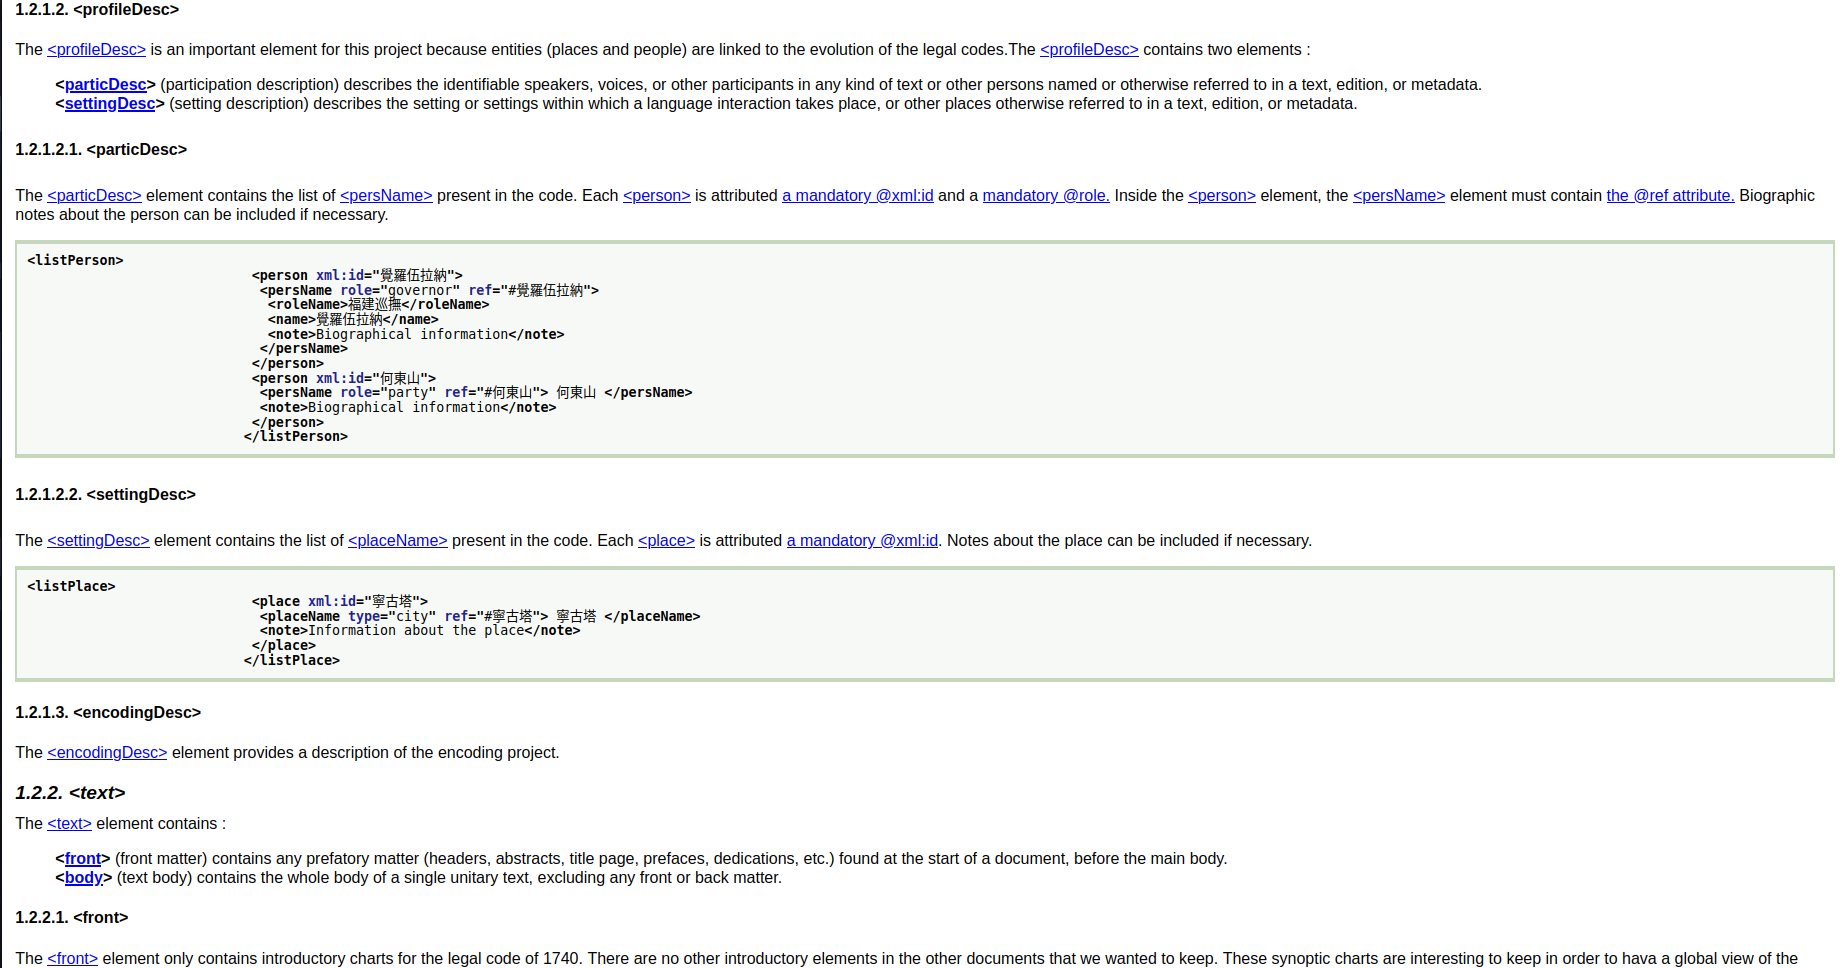
\includegraphics[width=\textwidth]{images/odd.png}
    \caption{Capture d'écran du guide d'encodage en \HTML}
\end{figure}

La page \HTML de sortie présente un sommaire puis la documentation rédigée ainsi que les règles de validation du document \TEI. Une mise en page similaire à celle des \textit{guidelines} est obtenue. Des liens hypertextes permettent de naviguer dans le guide depuis la table des matières, vers la documentation en prose et les règles de validation, retranscrites sous forme de tableau comme dans les \textit{guidelines}.

\begin{figure}
    \centering
    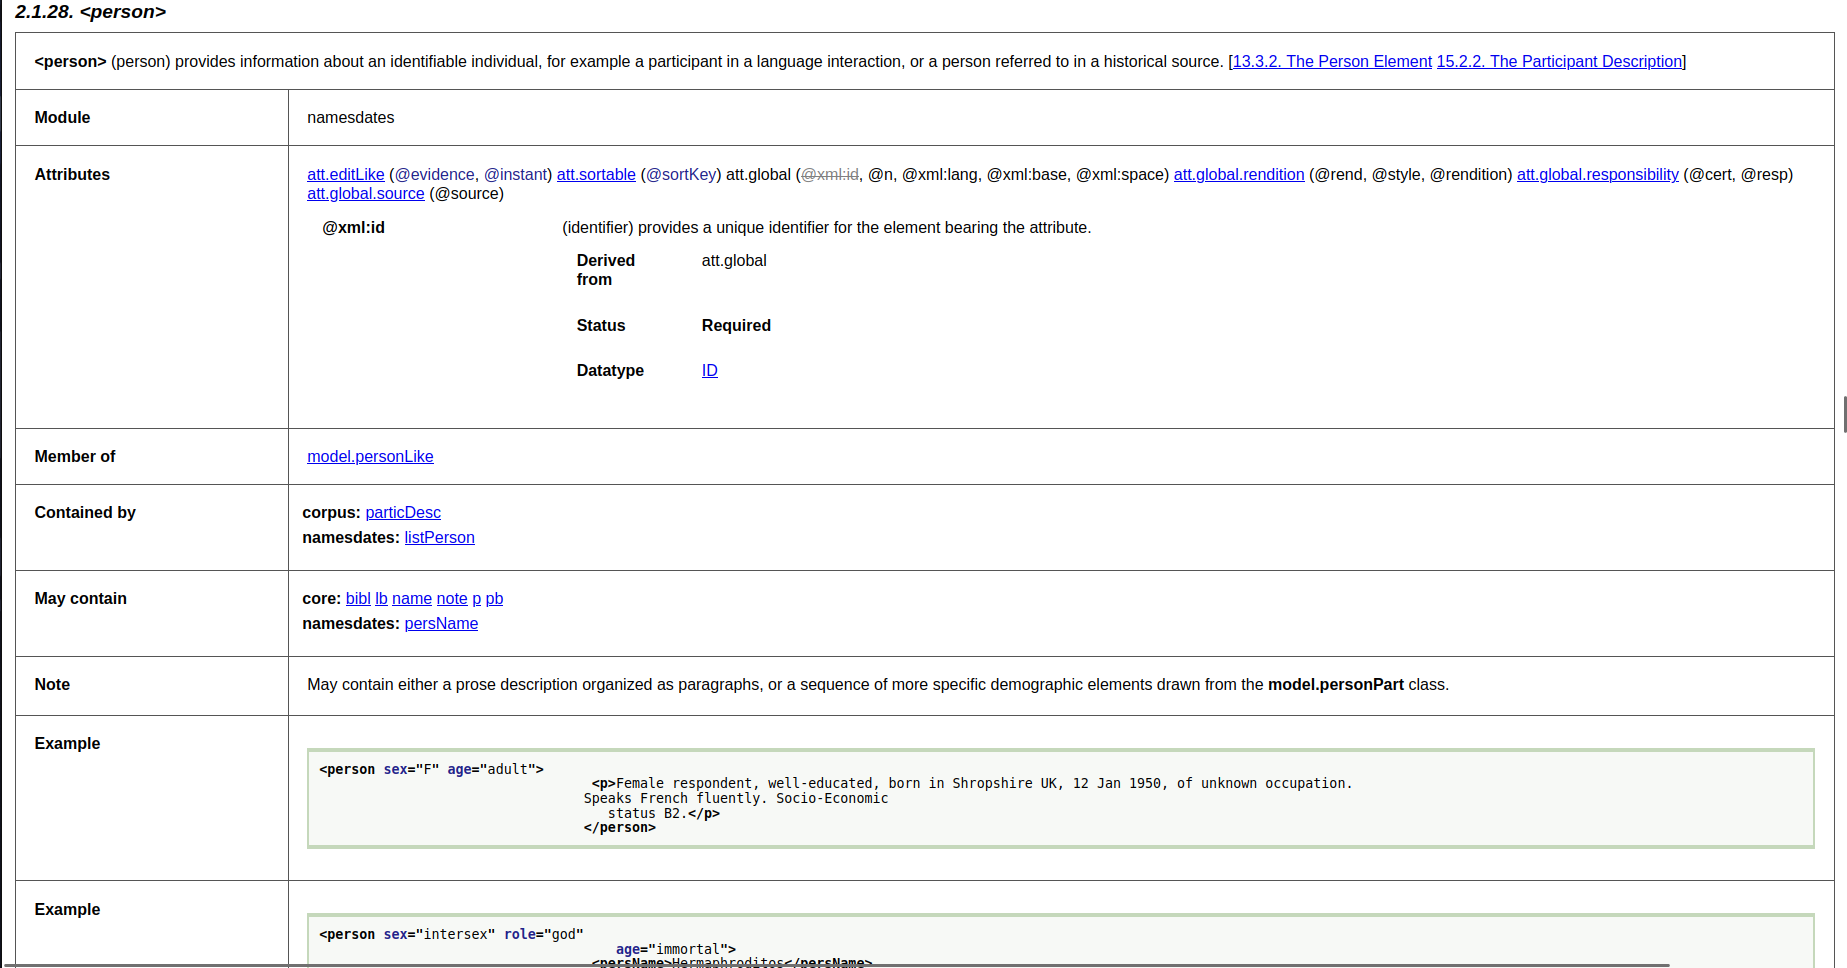
\includegraphics[width=\textwidth]{images/odd2.png}
    \caption{Capture d'écran des règles de validation en \HTML}
\end{figure}

Le scénario \textit{oddbyexample} fournit également en sortie un fichier \RNG afin de le lier aux documents \TEI pour mettre en place un schéma de validation.

\newpage
\subsection{Le schéma de validation}

L'\ODD permet également de rédiger des règles de validation afin de faciliter l'encodage en \TEI et de mettre en lumière les informations manquantes ou mal encodées. En effet, la mise en place d'un schéma de validation permet, via le logiciel \textit{Oxygen}, de faire apparaître les erreurs via un code couleur : rouge pour les erreurs de première importance, et orange pour les manquements de l'encodage. 

Plusieurs règles d'encodage ont donc été définies à partir des documents du corpus ainsi que l'échantillon. Les textes de lois suivant une structure rigoureuse, les éléments \texttt{<div/>} ont fait l'objet de règles strictes afin de garantir que les erreurs de structure ou d'imbrication des éléments soient repérées : 

\begin{minted}{xml}
    <!-- Il doit y avoit 7 chapitres -->
    <constraintSpec scheme="schematron" ident="sequence" xml:id="rule05">
        <constraint>
            <s:rule context="tei:body">
                <s:assert test="count(tei:div[@type='chapter'])=7"> 
                Il doit y avoir 7 chapitres dans le document. 
                </s:assert>
            </s:rule>
        </constraint>
    </constraintSpec>
\end{minted}

Afin de pouvoir rédiger des règles sur certains types d'éléments \texttt{<div/>} uniquement, la syntaxe \textit{Schematron} a été utilisée. Les règles \textit{Schematron} permettent de donner dans l'attribut \texttt{@context} un chemin \xpath. Ainsi, la règle ci-dessus ne s'applique qu'aux éléments \texttt{<div/>} directement contenues dans la balise \texttt{<body/>}. Ces divisions qui correspondent aux chapitres des textes de loi sont obligatoirement au nombre de sept. La syntaxe \textit{Schematron} a ainsi permis d'indiquer que chaque chapitre doit contenir une ou plusieurs sections, devant elles-mêmes contenir des \lu. Les règles de validation garantissent que la structure des documents orignaux est bien respectée et régulière tout au long de l'encodage. Ces règles de validation sont essentielles afin de publier une édition scientifique numérique utilisable par les chercheurs, dans le respect de l'architecture des codes légaux chinois. 

Certains éléments, en revanche, sont spécifiques à notre projet d'édition et ne sont pas primordiaux afin de réaliser les livrables du projet, comme par exemple l'intégration des images en regard du texte. Ces éléments sont importants pour remplir les objectifs du projet puisqu'inclure la numérisation des codes légaux dans le site web fait partie du périmètre. Toutefois, il ne s'agit pas d'erreurs de même niveau qu'un problème de structuration des textes, c'est pourquoi deux niveaux d'erreurs ont été distingués : 

\begin{minted}{xml}
    <constraintSpec scheme="schematron" ident="facs" xml:id="rule08">
        <constraint>
            <s:rule context="tei:body//tei:pb">
                <s:assert test="@facs" role="WARN"> 
                    L'attribut facs est obligatoire 
                </s:assert>
            </s:rule>
        </constraint>
    </constraintSpec>
\end{minted}

Dans la règle ci-dessus, l'attribut \texttt{@role} permet de spécifier que la règle concernant l'ajout de l'attribut \texttt{@facs} pour l'intégration des images est obligatoire mais que le niveau d'erreur est inférieur à la règle précédente. La règle a donc un rôle d'\og avertissement \fg. Dans l'éditeur \textit{Oxygen}, elle apparaît en orange afin de la distinguer des erreurs de niveau supérieur.
 \begin{figure}
     \centering
     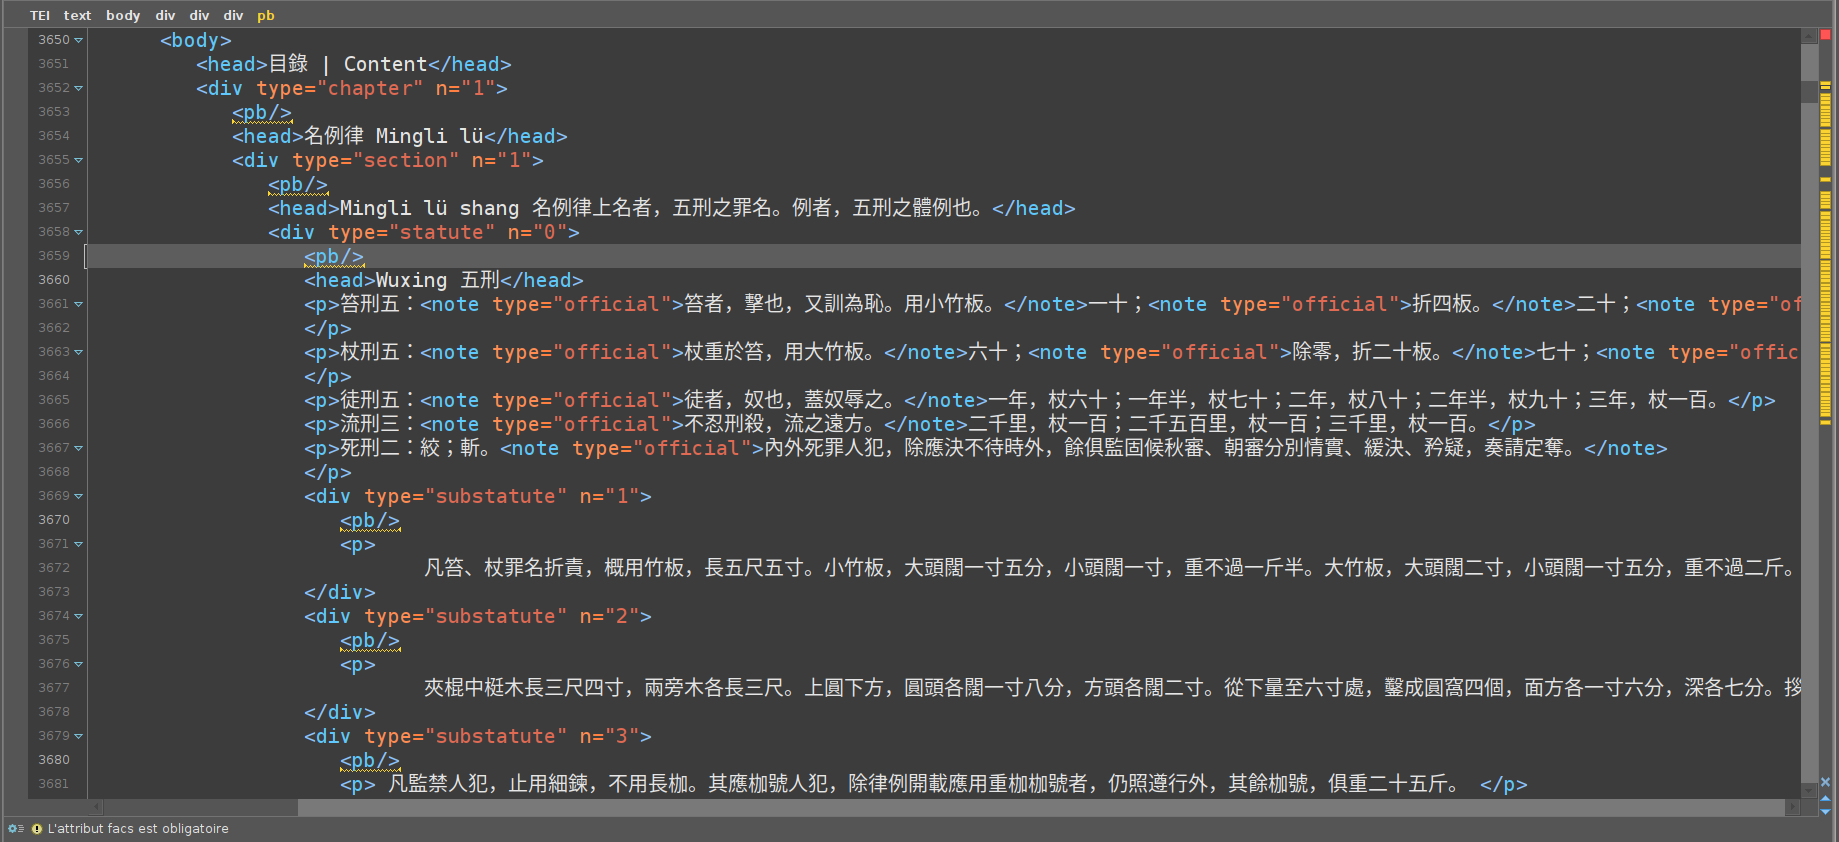
\includegraphics[width=\textwidth]{images/oxygen.png}
     \caption{Capture d'écran de l'affichage des erreurs sur Oxygen}
 \end{figure}

 \newpage
 C'est également dans l'\ODD qu'il est possible de modifier les règles de validation afin d'étendre la \TEI. Dans le cadre de la création d'un code légal généré automatiquement pour chaque année de la dynastie Qing, il est nécessaire d'encoder des périodes de validité pour chaque \lu et \li. Les attributs \texttt{@notBefore} et \texttt{@notAfter} ne sont pas autorisés sur les éléments \texttt{<div/>}. La rédaction des règles de validation a donc permis d'ajouter ces attributs sur les divisions souhaitées. Pour cela, les attributs ont été ajoutés dans la liste des attributs autorisés sur l'élément \texttt{<div/>} : 

 \begin{minted}{xml}
    <attList>
        <attDef ident="notBefore" mode="add"/>
        <attDef ident="notAfter" mode="add"/>
    </attList>
 \end{minted}

En plus de cet ajout, une règle \textit{Schematron} a été rédigée afin de spécifier que ces attributs sont obligatoires sur les \lu et les \li. 

Une fois le schéma d'encodage défini et les règles rédigées, la transformation via le scénario \textit{oddbyexample} a créé un fichier \RNG qui doit être lié aux documents \TEI comme ceci : 

\begin{minted}{xml}
<?xml-model href="ODD_COREL.rng" type="application/xml" 
schematypens="http://relaxng.org/ns/structure/1.0"?>
<?xml-model href="ODD_COREL.rng" type="application/xml" 
schematypens="http://purl.oclc.org/dsdl/schematron"?>
\end{minted}

L'éditeur \textit{Oxygen} prend ensuite en compte le schéma d'encodage défini et permet de souligner les erreurs selon les différents niveaux. Ces règles de validation sont essentielles afin de permettre à l'équipe du projet de poursuivre l'encodage et atteindre le modèle de données souhaité. La création de règles de validation permet de mettre en avant les données manquantes dans les documents et de guider l'ajout des données, ce qui assure un encodage régulier et cohérent au sein d'un texte, mais aussi d'un document à un autre. De plus, ce document peut s'avérer utile pour l'édition en \TEI d'autres textes de lois chinois et permet d'offrir à la fois une documentation claire et un outil de validation qui garantit l'obtention d'un document valide. Grâce à l'\ODD, le projet \COREL peut ainsi se détacher du schéma d'encodage \LSC initial et encoder directement les informations à ajouter et/ou de nouveaux documents en \TEI. Il est également possible de modifier l'\ODD pour ajouter de nouvelles règles si le projet d'encodage évolue dans le temps. 

             
            
        \clearemptydoublepage

    \part{La mise à disposition des données pour les chercheurs : comment agréger des sources partielles grâce au numérique ?}
    \chapter{Les bases de données document pour agréger des sources partielles}
                    \section{Pourquoi choisir une base de données document ? }
    \subsection{Les avantages d’une base de données document}
    
Le c\oe ur du projet \COREL est l'éditorialisation d'un corpus de textes juridiques. Une base de données orientée document permet de mettre en avant les documents au même plan que les informations qu'ils contiennent, ce qui est essentiel à un projet d'édition scientifique numérique. De plus, ces bases de données sont généralement structurées au format \XML ou \JSON. Le choix de ce type de base de données entrait donc en concordance avec les données initiales du projet qui se composaient essentiellement de ces deux formats. Par ailleurs, ce choix a également été motivé pour sa praticité : les données étant déjà structurées, la mise en place d'une base de données document ne demandait aucune étape supplémentaire, contrairement à la mise en place d'une base de données relationnelle. 

Toutefois, la mise en place d'une base de données relationnelle n'est pas à exclure sans réflexion. En effet, le projet \COREL vise à mettre en relation des textes et des lois entre eux. Une base de données sous forme de tables, avec des tables de relation, n'est pas sans pertinence pour un tel projet et aurait permis de faciliter la modélisation des liens entre les lois. La mise en relation des lois entre elles à l'aube du projet était représentée par un référencement complexe de liens hypertextes à partir du \genyuan. Afin de consulter les lois liées les unes aux autres à partir de ce référentiel, il est nécessaire de naviguer entre le serveur \IIIF et le référentiel et de multiplier les allers et retours. Une base de données relationnelle aurait permis aux chercheurs en humanités numériques de requêter directement en \SQL. 

La mise en place d'une base de données relationnelle est donc loin d'être inintéressante. Cependant, cette solution ne répondait pas pleinement aux besoins du projet. Bien que le requêtage d'une base de données, pour des documents partageant des liens complexes d'association et de généalogie, soit très intéressant du point de vue des humanités numériques, il n'aurait sans doute pas été exploité par la communauté ciblée par le projet \COREL, les chercheurs en histoire du droit chinois et les sinologues. L'objectif du projet est non seulement de rassembler et de lier ces sources fragmentées et partielles, mais surtout d'en faciliter l'accès et l'exploitation par les chercheurs. La mise en relation des textes et lois entre eux sans l'appui d'outils numériques est un travail long et fastidieux, comme l'a démontré le référentiel mis en place en regard des numérisations des sources. Une base de données relationnelle n'aurait ainsi pas pleinement servi l'objectif du projet : recréer artificiellement un code légal similaire aux sources originales, directement accessible et consultable afin de faciliter le travail de recherche. De plus, la restructuration des sources numériques en une base relationnelle aurait demandé des étapes de restructuration des données supplémentaires. 

Une base de données document, en revanche, offre la possibilité de mettre en relation les lois tout en conservant la structuration du document telle que la connaissent les chercheurs, rendant son exploitation plus instinctive pour le public cible. 

\subsection{Un système de gestion de base de données}

La gestion d'une base de données s'appuie sur un \SGBD. Dans TEI Publisher, un \SGBD est directement intégré à l'application, permettant d'administrer les données du site web (eXist-db) et une \IDE (eXide). Ces outils, à l'instar de TEI Publisher, sont disponibles en ligne à l'installation, documentation à l'appui, ou directement à l'essai, comme c'est le cas pour eXide. Si les chercheurs ne seront pas amenés à coder directement dans eXide en XQuery, le \SGBD est un outil indispensable à la gestion du site web du projet, puisque le site doit continuer d'être alimenté après l'échéance du financement. En plus de bénéficier d'une documentation solide, eXist-db possède une interface simple et facile à prendre en main pour les chercheurs.

En effet, jusqu'à ce jour, les chercheurs continuent d'alimenter le site internet du projet \LSC via \FTP depuis l'éditeur \XML Oxygen et ont donc déjà une expérience de gestion de base de données document. L'interface d'eXide, en plus d'être similaire à Oxygen, propose les mêmes fonctionnalités directement dans TEI Publisher, ce qui simplifie le processus d'ajout ou de modification des documents, puisque les chercheurs devaient naviguer entre Oxygen et le site web \LSC pour mettre à jour à la fois les documents (directement en \XML) et le site (via un bouton \og process \XML \fg). 

 \section{La reconstitution de la législation grâce au XQuery}
    \subsection{La chaîne de traitement envisagée}
L'\IDE, en plus d'offrir aux chercheurs une interface de modifications des données \XML pour mettre à jour les documents, permet également aux développeurs de l'application d'intervenir sur le code source afin de le personnaliser. En effet, le site web du projet pourra se développer essentiellement en interface graphique grâce à TEI Publisher en ce qui concerne la génération des pages \HTML pour l'édition des documents, mais la reconstitution de la législation à partir des sources nécessite de filtrer les données un peu plus précisément. 

Le langage XQuery est un langage de requête qui permet notamment d'interroger une base de données document. Dans le cadre du projet, le XQuery sera utilisé pour filtrer les données \XML par date, afin de reconstituer la législastion pour une date donnée par l'utilisateur. Cette requête, simple en apparence, demande d'intervenir directement sur le code plutôt que de filtrer par prédicat comme il est possible de le faire dans l'interface de TEI Publisher, car les résultats seront générés à la volée, selon la date entrée par l'utilisateur. Prévoir à l'avance le filtrage des données année par année, de 1644 à 1911, en utilisant un prédicat surchargerait le code de l'application et demanderait un travail trop conséquent. 

Les bornes chronologiques de validité de chaque loi étant encodées grâce aux attributs @notBefore et @notAfter, la requête permettra de déterminer si la date donnée en entrée est comprise entre les dates de début et de fin. Si c'est le cas, la loi sera affichée dans la reconstitution du code virtuel, avec à la suite les lois secondaires qui y sont rattachées, elles-aussi filtrées selon leur période de validité.

\subsection{Déterminer les bornes du corpus}

Avant de déterminer la manière de requêter en XQuery pour recréer la législation, il a fallu déterminer les bornes chronologiques réelles des lois présentes du corpus. En effet, la dynastie des Qing s'étend de 1644 à 1911, mais la législation n'a, de fait, pas brutalement été créée en 1644. La loi évolue sous l'influence des époques et se reconstruit sur les bases de la dynastie précédente. En l'occurrence, la législation des Qing est étroitement liée à celle des Ming et certaines lois présentes dans le corpus sont antérieures à 1644. Si le projet \COREL ne vise qu'à étudier la législation sous la dynastie Qing, il est toutefois impossible d'ignorer ses origines plus anciennes. Déterminer les bornes chronologiques d'un corpus d'études relève nécessairement de l'arbitraire. C'est pour cette raison qu'une étude plus approfondie du corpus a été nécessaire, afin d'établir dans un premier temps quelles étaient les bornes chronologiques réelles des lois du corpus. 

Une requête en XQuery a permis de lister toutes les dates présentes dans le \huidian, le seul document du corpus à posséder des dates à l'heure actuelle. 
\bigskip
\begin{minted}{xquery}
declare namespace tei="http://www.tei-c.org/ns/1.0";
for $date in distinct-values( doc("db/TEI_HDSLXB.xml")//tei:date/text())
order by $date
return $date
\end{minted}
\bigskip
Le résultat permet d'établir que la date la plus ancienne mentionnée dans le \huidian est 1616, soit presque trente ans avant le début de notre corpus. Bien que la recréation de la législation dans le cadre du projet \COREL concerne strictement les bornes chronologiques de 1644 à 1911, ce résultat amène à la réflexion suivante : comment retracer la généalogie complète d'une loi en limitant artificiellement les bornes chronologiques du corpus à la dynastie Qing ? Considère-t-on que ces dates arbitraires servent de délimiteurs stricts et que tout ce qui en dépasse le cadre doit être ignoré pour mener à bien le projet ? En suivant cette perspective, il serait alors logique, dans l'encodage, de remplacer toute date antérieure à 1644 par celle-ci. Ce choix pose toutefois un problème d'altération des sources. Le choix de bornes chronologiques propose à l'historien de présenter ses sources à travers un prisme, une vue subjective et personnelle, qui peut parfois sembler injustifiée.

Pour résoudre ce problème, il semble \textit{a priori} que conserver des dates antérieures au début du corpus ne complexifie pas la recréation de la législation sous les Qing. En effet, le site web peut spécifier à l'utilisateur que la génération d'un code légal artificiel n'est valable que pour des bornes chronologiques prédéfinies, en utilisant uniquement les textes de lois produits durant cette période. Toutefois, qu'en est-il des dates de fin ? Tout comme le droit n'est pas soudain apparu en 1644, il n'a pas pris fin en 1911. S'il est possible de trouver des références à la dynastie précédente dans les codes légaux des Qing, il est évident qu'aucune mention du futur n'est présente dans les textes. Pour assurer la cohérence de cette vision subjective de l'histoire, ne faudrait-il pas conserver la date réelle de fin de validité des lois ? Assurément, une telle entreprise ne peut être menée à l'échelle d'un projet : cela demanderait d'outrepasser le corpus prédéfini et d'y inclure des textes postérieurs à 1911, voire d'élargir démesurément le corpus jusque nos jours. De plus, le droit vivant n'ayant jamais de fin, un projet d'une telle envergure serait également infini. Cette problématique est au centre de l'édition scientifique numérique. Elena Pierazzo en fait part à propos de l'édition diplomatique : 

\begin{quote}
    So, we must have limits, and limits represent the boundaries within which the hermeneutic
process can develop. The challenge is therefore to select those limits that allow a model
which is adequate to the scholarly purpose for which it has been created.
\footnote{\cite{pierazzo_rationale_2011}}
\end{quote}

Cette question de cadre ne peut ainsi être résolue par le numérique, qui laisse ouvertes toutes les possibilités, et requiert une intervention humaine et arbitraire. Peut-on considérer que les dates indiquées dans l'encodage n'altèrent en rien la source, qu'elles ne sont que la nécessité d'un projet numérique ? Les réponses sont multiples et chacune n'en est pas moins valide. Dans le cadre du projet, l'édition des codes légaux n'est pas une édition diplomatique. Dès lors, il a été choisi d'utiliser des dates arbitraires pour l'encodage, afin d'assurer la bonne réalisation du projet. De la même manière, des identifiants \XML seront ajoutés à l'encodage \TEI pour permettre de dédoublonner les lois. Ainsi, une même loi du \huidian et du \dc porteront le même identifiant, peu importe le texte d'origine. Ce choix peut sembler peu satisfaisant d'un point de vue scientifique et altérer les sources, mais la reconstitution de codes légaux est artificielle et doit se considérer comme étant la production d'une source nouvelle, autre, qui n'altère en rien les sources originales. 

            
        \clearemptydoublepage
        
        \chapter{La mise en place d’un outil open source pour les chercheurs}
                    \section{Conception d'une plateforme pour les chercheurs}
    \subsection{Utilisation des sources du droit chinois en humanités numériques}

L'accès aux sources du droit chinois, au croisement entre les disciplines que sont l'histoire et le droit, est encore peu développé. Les collections de la bibliothèque d'études chinoises du \cdf contient les textes de lois du corpus du projet mais la bibliothèque étant en travaux, la consultation sur place n'est possible que sur rendez-vous. Sur le web, certains projets proposent un accès aux sources mais celles-ci restent majoritairement partielles. Le projet \LSC  propose une édition trilingue des codes légaux chinois de la dynastie Qing, cependant les données ne sont pas complètes à l'heure actuelle et les documents sont toujours en cours de saisie sur le site internet. Le projet de recherche japonais \textit{Terada's Homepage for Chinese Legal History Studies in Japan} \footnote{http://www.terada.law.kyoto-u.ac.jp/index_en.htm} de l'Université de Kyoto propose une édition du \dc uniquement. Or, l'étude du droit chinois et de son évolution nécessite la consultation simultanée des différents textes de lois. La conception d'un site web réunissant ces sources dans leur intégralité afin de faciliter l'accès aux chercheurs est donc au centre du projet \COREL. 

De plus, ces projets de recherche offrent uniquement un accès à leur édition en ligne, mais l'histoire du droit chinois est une discipline peu développée en humanités numériques. Les données et leur éditorialisation ne sont que peu diffusées en \textit{open access}. La production de données \textit{open source} par le projet \COREL cherche à permettre aux humanités numériques de s'approprier ce terrain de recherche et de favoriser le développement de projets de recherche sur la généalogie du droit. Cependant, des outils \textit{open source} se développent peu à peu dans les projets d'humanités numériques. La version bêta de \textit{MARKUS}, en cours de développement par l'Université de Leyde aux Pays-Bas, permet le balisage et le référencement des entités nommées pour les textes chinois. Dans le cadre du projet \COREL, nous avons également testé le script \textit{Chinese Calendar Tools} \footnote{https://gitlab.com/vandenbosch.nora/chinesecalendartools/-/tree/main}, qui permet de convertir les dates du calendrier luni-solaire chinois \footnote{Le calendrier luni-solaire, utilisé par plusieurs cultures, est un calendrier combinant le calendrier lunaire et solaire.} vers des dates du calendrier grégorien. Bien que l'échéance du financement n'ait pas permis d'exploiter ces deux outils \textit{open source} afin d'enrichir l'encodage des sources, ils permettent de démontrer que les études chinoises dans les humanités numériques en Europe se développent peu à peu. Le projet \COREL s'inscrit dans cette démarche de science ouverte et contribue avec l'éditorialisation du corpus de codes légaux de la dynastie Qing et la mise à disposition en \textit{open access} de ces données, au développement des projets d'humanités numériques pour les études chinoises. 

\subsection{Les enjeux de la reconstitution de la législation}

Offrir une édition scientifique numérique complète des textes légaux sous la dynastie Qing est donc un projet conséquent qui ambitionne de faciliter l'accès aux sources par les chercheurs, en concevant une plateforme unique réunissant les sources pour une consultation simultanée des textes. L'édition numérique permet à la fois de réunir les différents volumes d'un même code légal, mais aussi de proposer sur le même site web toutes les sources de droit chinois sous la dynastie Qing dont dispose le projet.

Toutefois, l'éditorialisation du corpus n'est qu'une partie du projet \COREL. En effet, l'équipe souhaite reconstituer la législation de 1644 à 1911, pour chaque année de la dynastie Qing. La recréation d'un texte de loi, généré automatiquement à la demande des utilisateurs, permettrait de faciliter l'accès aux sources à un niveau supérieur. À l'instar des nombreuses compilations rédigées sous la dynastie Qing, le \cv permettrait de compiler en temps réel toutes les lois valides pour une année donnée. Cet aspect du projet vise à faciliter les recherches de l'évolution du droit par le numérique : plutôt qu'un travail de recherche comparatif entre les différents textes, les chercheurs auront accès à la reconstitution de la législation grâce à l'agrégation de toutes ces sources, directement sur le web, en libre accès. 

Enfin, la reconstitution de la législation s'accompagne d'un travail sur la généalogie des lois. Les visualisations via les liens d'association dirigée entre les lois permettront également de faciliter le travail de recherche en retraçant la généalogie d'une loi en entier, sans nécessité de naviguer entre les différentes sources partielles. En effet, pour étudier la généalogie des lois, une étude de toutes les sources est nécessaire afin de trouver toutes les versions de la loi et ses modifications dans le temps, jusqu'à son abrogation. Aucun accès immédiat à la généalogie complète d'une loi n'est disponible dans les textes, puisque toutes les sources sont partielles et se complètent les unes les autres. Le projet \COREL ambitionne donc d'aider les chercheurs en facilitant ce travail de recherche sur la généalogie des lois. 

\subsection{Définition des besoins utilisateurs}

Le public cible du projet étant les chercheurs en histoire du droit chinois, il est possible d'établir des besoins utilisateurs précis pour le projet \COREL. D'une part, les chercheurs doivent pouvoir accéder à l'édition scientifique numérique des sources sur le site web, avec une structure des textes qui leur est familière, c'est-à-dire que l'édition des textes de lois doit se faire, à l'instar de la source originale, en chapitres et sections. Chaque chapitre, sections et les différentes lois doivent être numérotés afin de se repérer dans les textes. Les chercheurs ont aussi besoin de pouvoir naviguer entre les différents textes, le corpus se prêtant à de la consultation plutôt qu'à une lecture continue et linéaire. Une table des matières cliquable et qui indique la position actuelle de l'utilisateur doit donc être créée. 

En plus de l'édition en ligne, les utilisateurs doivent pouvoir accéder à la recréation de la législation, le \cv, afin de pouvoir accéder à un texte de loi composite pour une année entre 1644 et 1911. Un format \pdf doit être disponible au téléchargement pour être consulté hors connexion. Cette reconstitution de la législation doit respecter la mise en page d'un texte de lois, c'est-à-dire qu'il doit présenter les chapitres et sections usuels. Le besoin des chercheurs n'est pas de filtrer simplement les données par dates, mais de conserver la structure des codes afin de pouvoir consulter, par exemple, les lois selon les ministères auxquels elles sont rattachées, ou encore les \li selon la loi principale qu'elles viennent compléter. 

Enfin, une modélisation des liens d'association dirigée entre les lois est essentielle afin de faciliter les travaux de recherche et d'offrir une compréhension instantanée de la généalogie d'une loi. En effet, le fichier de référencement des liens entre les lois tels qu'il existe actuellement pour appuyer le projet demeure difficile d'appréhension à la première lecture et demande de naviguer via les liens hypertexte. La lecture de ce document, qui n'est pas continue, ne permet pas de saisir immédiatement la généalogie d'une loi. Apporter des visualisations aux utilisateurs est donc un besoin primordial afin de faciliter les recherches sur la généalogie des lois et leur évolution. 

Afin de répondre aux besoins des chercheurs, qu'ils soient utilisateurs ou administrateurs, il est important de concervoir une plateforme adaptée, en libre accès, afin de contribuer au développement de l'histoire du droit chinois en humanités numériques.

 \section{La publication de données en ligne : un travail accessible à un plus large public}
    \subsection{L’outil TEI Publisher}
\tp est un outil de publications de données encodées en \TEI, qui s'appuie sur le système de gestion de base de données \XML \textit{eXist-db}. C'est un outil \textit{open source} qui propose de construire une édition en ligne, essentiellement en interface graphique. Des templates \HTML sont ensuite générés, ce qui permet aux chercheurs de publier leurs corpus de recherche édités en codant le moins possible. Il est également possible de publier d'autres langages via  \tp : le \XML Docbook, \JATS ou encore les fichiers .docx. L'outil \tp respecte des standards afin de faciliter l'échange des données et les principes \fair en utilisant les langages \XML (\TEI, \ODD, XQuery). La construction d'un site web à partir de l'application \tp est possible grâce à la génération des templates \HTML et de l'utilisation des \textit{webcomponents}, qui font partie des spécifications \HTML 5 afin de personnaliser le site web. Afin d'offrir un haut niveau de personnalisation tout en garantissant la pérennité des sites web construits à partir de \tp, l'application propose d'utiliser les \textit{webcomponents} comme des briques individuelles à ajouter et assembler selon les besoins utilisateurs. 

L'usage de \tp se démocratise de plus en plus dans les projets en humanités numériques. Le site web du projet \cordel (mais aussi les projets menés par l'INRIA), a été construit via \tp. L'utilisation de \tp a donc été envisagée dès le début du stage, afin d'organiser une veille sur cet outil. Cette veille s'est organisée en trois temps : 

\begin{itemize}
    \item La consultation de la documentation de \tp et des applications réalisées, notamment \cordel et \disco. 
    \item La réalisation de deux entretiens avec Hugo Scheithauer (en visioconférence) et Floriane Chiffoleau (à l'INRIA). 
    \item Un test via l'\og aire de jeux \fg de \tp, qui permet de tester immédiatement les fonctionnalités de l'application en local. 
\end{itemize}

\subsubsection{La documentation}
\tp dispose d'une documentation complète \footnote{https://teipublisher.com/exist/apps/tei-publisher/doc/documentation.xml?odd=docbook\&view=div} consultable en ligne. En plus de la documentation écrite, il existe des cours en ligne, \og Stay home and learn \TEI from scratch \fg, proposé par \textit{e-editiones}, un groupe à but non lucratif qui oeuvre pour le développement de la science ouverte dans l'édition scientifique numérique. La documentation étant longue et exhaustive, cette première étape de la veille sur \tp s'est étalée sur plusieurs semaines en début de stage afin de se familiariser avec la méthodologie générale de la création d'un site web via \tp. La consultation ponctuelle de la documentation et des cours en ligne s'est par la suite révélée indispensable tout au long du stage, afin de compléter cette première approche, notamment lors de la mise en pratique. 

\subsubsection{Entretiens avec des professionnels}
En plus de la consultation de la documentation, j'ai mené deux entretiens à propos de \tp. Le premier, avec Hugo Scheithauer, à propos de l'application Data Catalogue, un projet d'édition scientifique numérique de catalogues de vente, m'a permis d'obtenir des informations générales sur la méthode de travail et la gestion d'un projet avec \tp : un tel projet est généralement mené en équipe de deux, avec un développeur \textit{front-end} et un développeur \textit{back-end}. L'utilisation de \tp, bien qu'en interface graphique, requiert des connaissances minimales en développement web et en langages \XML. M. Scheithauer a également souligné l'importance de la préparation des données avant le démarrage du projet. \textit{A priori}, avec toutes les données nécessaires identifiées et ajoutées dans l'encodage et une équipe de deux personnes, il est possible de créer un site web simple assez rapidement\footnote{Bien qu'il soit difficile d'estimer les délais de conception, qui sont propres à chaque projet, M. Scheithauer a indiqué qu'il envisageait un délai d'environ six mois pour se consacrer au développement d'une application simple, à partir d'une équipe de deux personnes}. Toutefois, si l'on souhaite un haut niveau de personnalisation pour le site web, il est probable qu'il soit nécessaire d'intervenir sur le code source de l'application directement.

Un second entretien avec Floriane Chiffoleau, à propos du projet \disco, m'a permis d'approfondir ma compréhension du fonctionnement de \tp et de découvrir les méthodes de travail derrière \disco. Mme Chiffoleau m'a parlé de sa propre expérience avec \tp : elle a consacré deux semaines à la consultation de la documentation de \tp, en ayant déjà une bonne maîtrise des langages \XML, puis un mois de tests de l'application. Elle m'a présenté les différents modes d'affichage des éditions \disco, chacun permettant de mettre en lumière des informations différentes. Trois modes sont présents sur l'application \disco : un mode pour l'édition critique, un pour l'édition diplomatique et enfin un mode permettant de mettre en valeur les entités nommées. Ce dernier mode est également envisagé à ce jour pour la réalisation du projet \COREL. 

\begin{figure}[h]
    \centering
    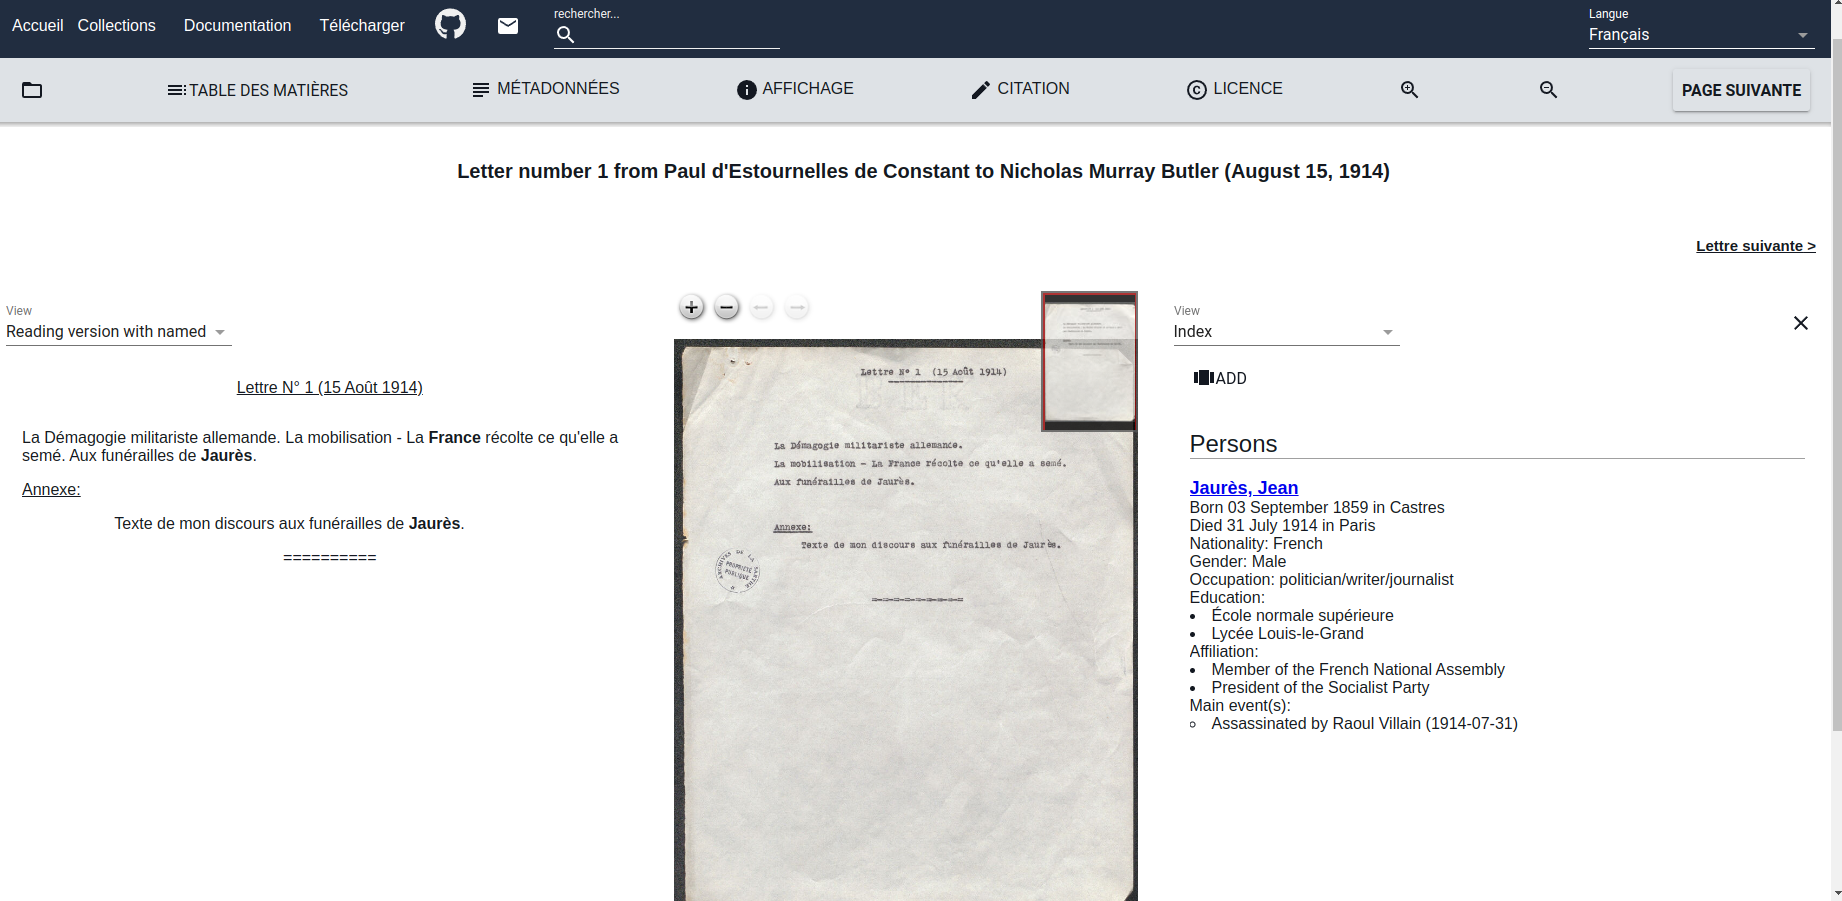
\includegraphics[width=\textwidth]{images/discholed.png}
    \caption{Capture d'écran du site web \disco}
\end{figure}

Lors de cet entretien, elle a également pu souligner l'importance d'encoder des documents \TEI valides, avec des règles de validations précises dans l'\ODD. En effet, si les documents ne respectent pas les mêmes règles de validation, cela complexifie le processus de conception de l'application, étant donné que \tp permet d'attribuer un comportement à un élément (par exemple, les balises \texttt{<note/>} du corpus \COREL s'affichent en bleu). Ainsi, respecter un schéma d'encodage défini permet de prévenir des erreurs d'affichages. 

Une fois ces deux premières étapes de veille menées à bien, l'aire de jeux \tp a permis d'effectuer un premier test avec le jeu de données \TEI de référence. 

\subsection{L’édition scientifique en interface graphique}

\tp permet en effet de construire son site web en interface graphique, grâce à une \ODD. L'\ODD \tp n'est pas à confondre avec l'\ODD qui permet de documenter un projet d'encodage et de définir des règles de validation. L'\ODD \tp est à distinguer d'une \ODD classique, puisqu'elle permet d'attribuer à un élément un comportement (\og behaviour \fg), c'est-à-dire une manière de s'afficher. Grâce à des requêtes XQuery générées automatiquement par \tp, les balises \TEI sont attribuées l'affichage souhaité sur le template \HTML. Il est possible de tester directement cette fonctionnalité grâce à l'aire de jeux de l'application \tp, une interface qui permet d'accéder à différentes \ODD d'exemples, comme pour les correspondances de Van Gogh ou les pièces de Shakespeare.\footnote{Les correspondances de Van Gogh et les pièces de Shakespeare sont deux éditions numériques publiées qui sont utilisées comme exemples par \tp.} L'aire de jeux donne l'accès aux \ODD et permettent de les modifier afin de tester les différentes possibilités d'affichage offertes par \tp. Il est possible de télécharger ses propres documents sur l'aire de jeux et de tester les \ODD disponibles, en les modifiant pour les adapter aux documents. Il est également possible de créer sa propre \ODD.

\begin{figure}[h]
    \centering
    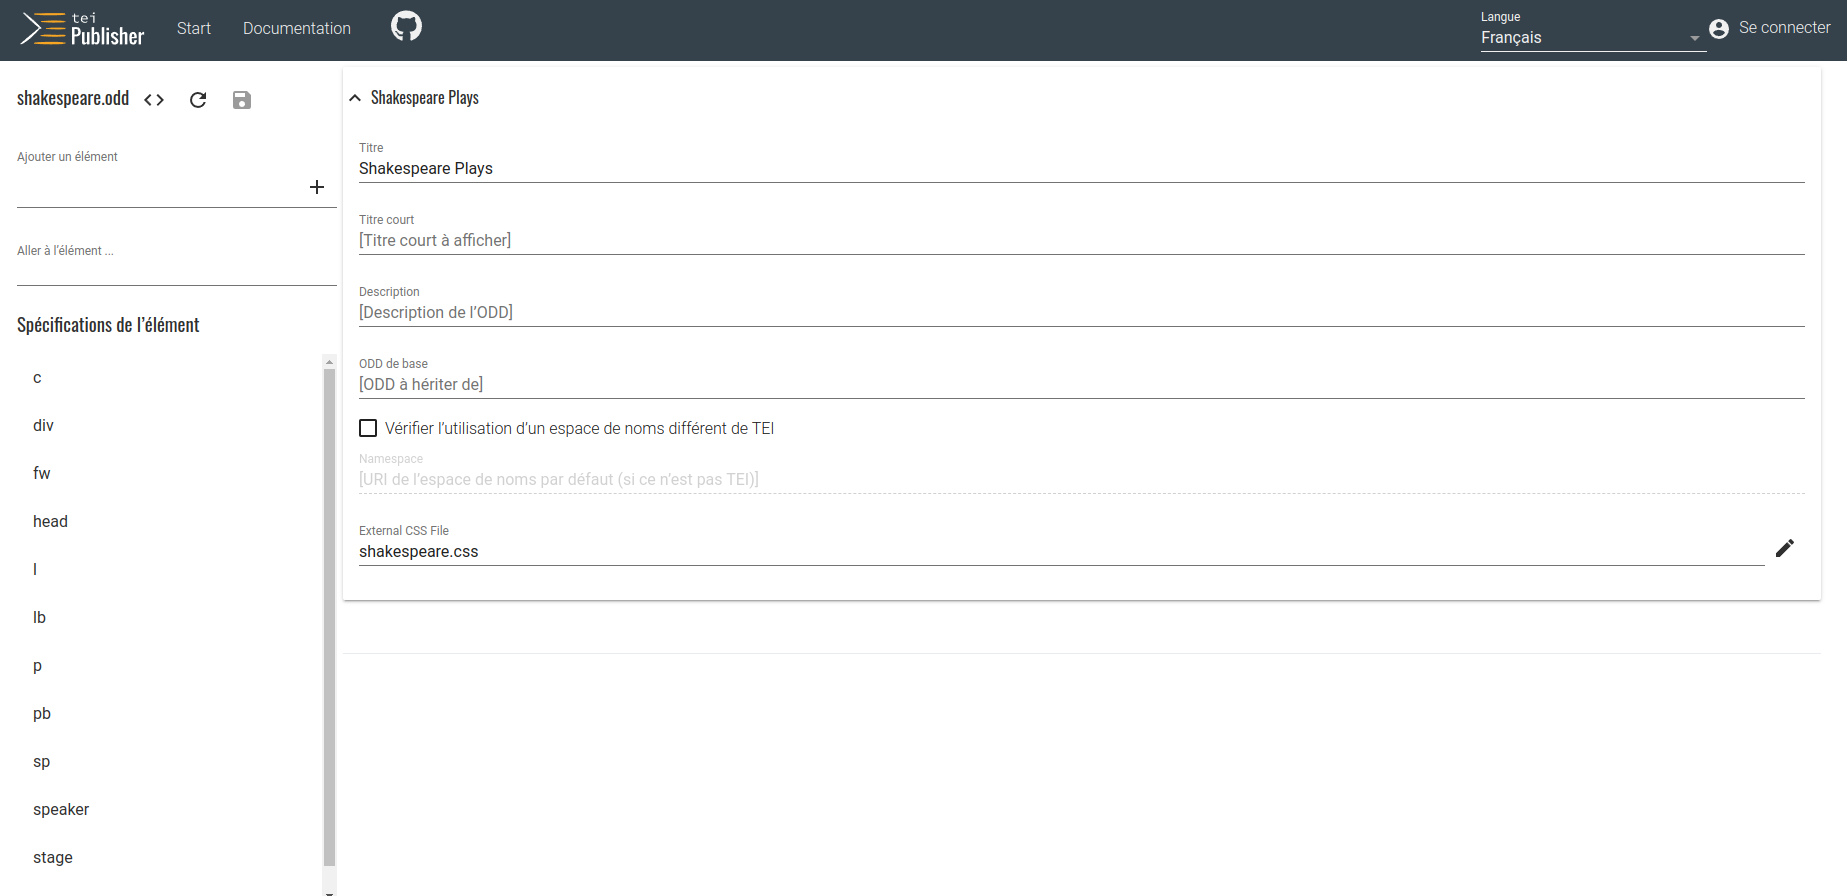
\includegraphics[width=\textwidth]{images/playground.png}
    \caption{Capture d'écran de l'aire de jeux \tp}
\end{figure}

La modification de l'\ODD est accessible intégralement en interface graphique. Ce mode d'édition est conseillé pour les débutants. Sur la gauche, il est possible de sélectionner les balises dont on veut modifier le comportement. Grâce à un chemin \xpath et à du code \CSS, \tp lance ensuite une requête XQuery qui applique le comportement choisi dans les templates \HTML générés automatiquement. 

\begin{figure}
    \centering
    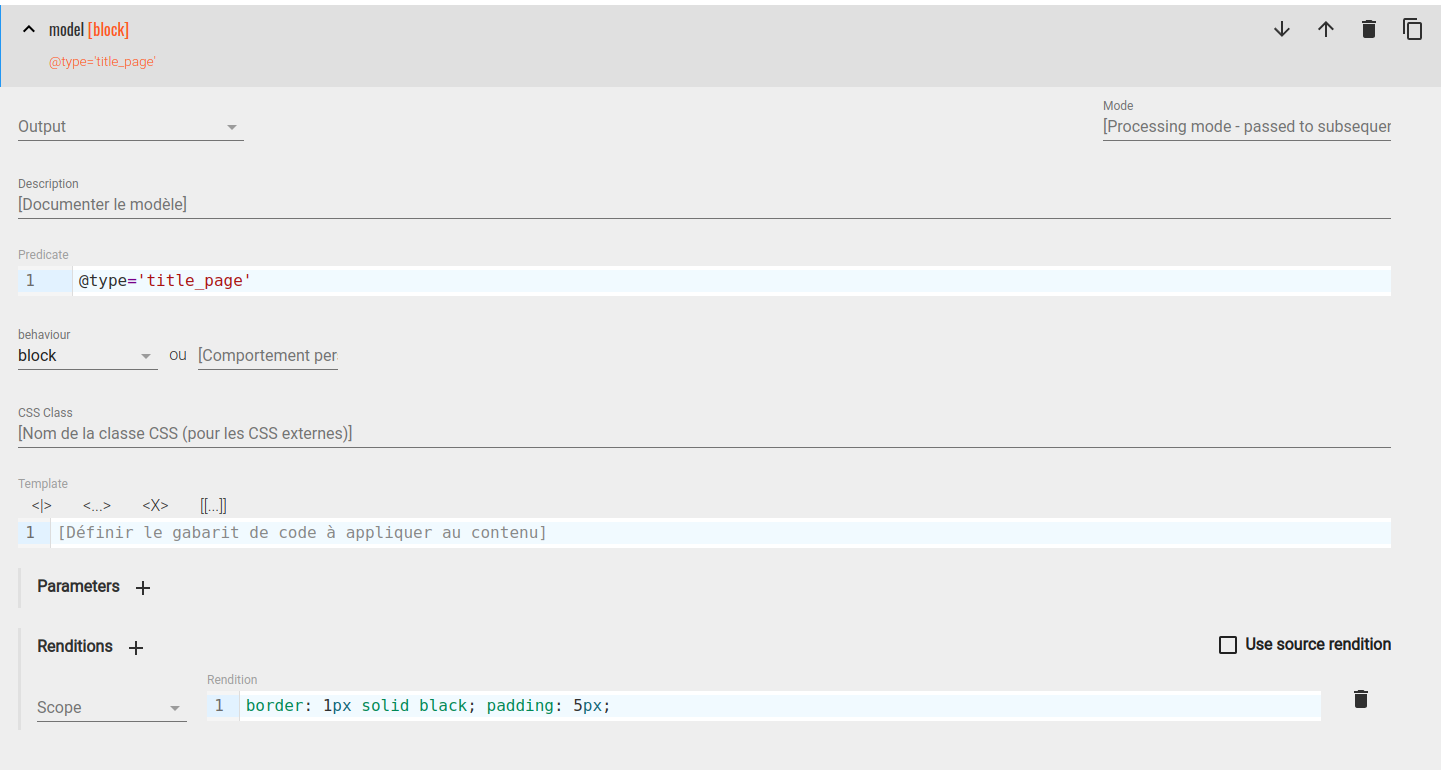
\includegraphics[width=\textwidth]{images/odd_playground.png}
    \caption{Capture d'écran de l'aire de jeux \tp : modifier le comportement d'un élément}
\end{figure}

Il est également possible d'éditer l'\ODD directement dans le code \XML. Ce mode d'édition nécessite cependant une connaissance avancée des langages \XML et une bonne compréhension du \textit{\TEI Processing Model}, qui est le langage derrière l'\ODD de \tp. Le \TEI Processing Model fait partie des \textit{guidelines} \TEI et leur documentation est donc accessible en ligne. 

L'objectif du projet \COREL étant de produire une édition scientifique numérique le plus possible en interface graphique, c'est le premier mode d'édition de l'\ODD qui a été jugé le plus pertinent pour le projet. Dans le cadre du stage, un premier test de cette fonctionnalité de \tp a donc été réalisé, afin de reproduire l'un des différents modes d'affichages souhaités pour le projet.\footnote{À propos de ces différents modes d'affichages, voire la partie concernée dans le cahier des charges, en annexes.} 

\begin{figure}[h]
    \centering
    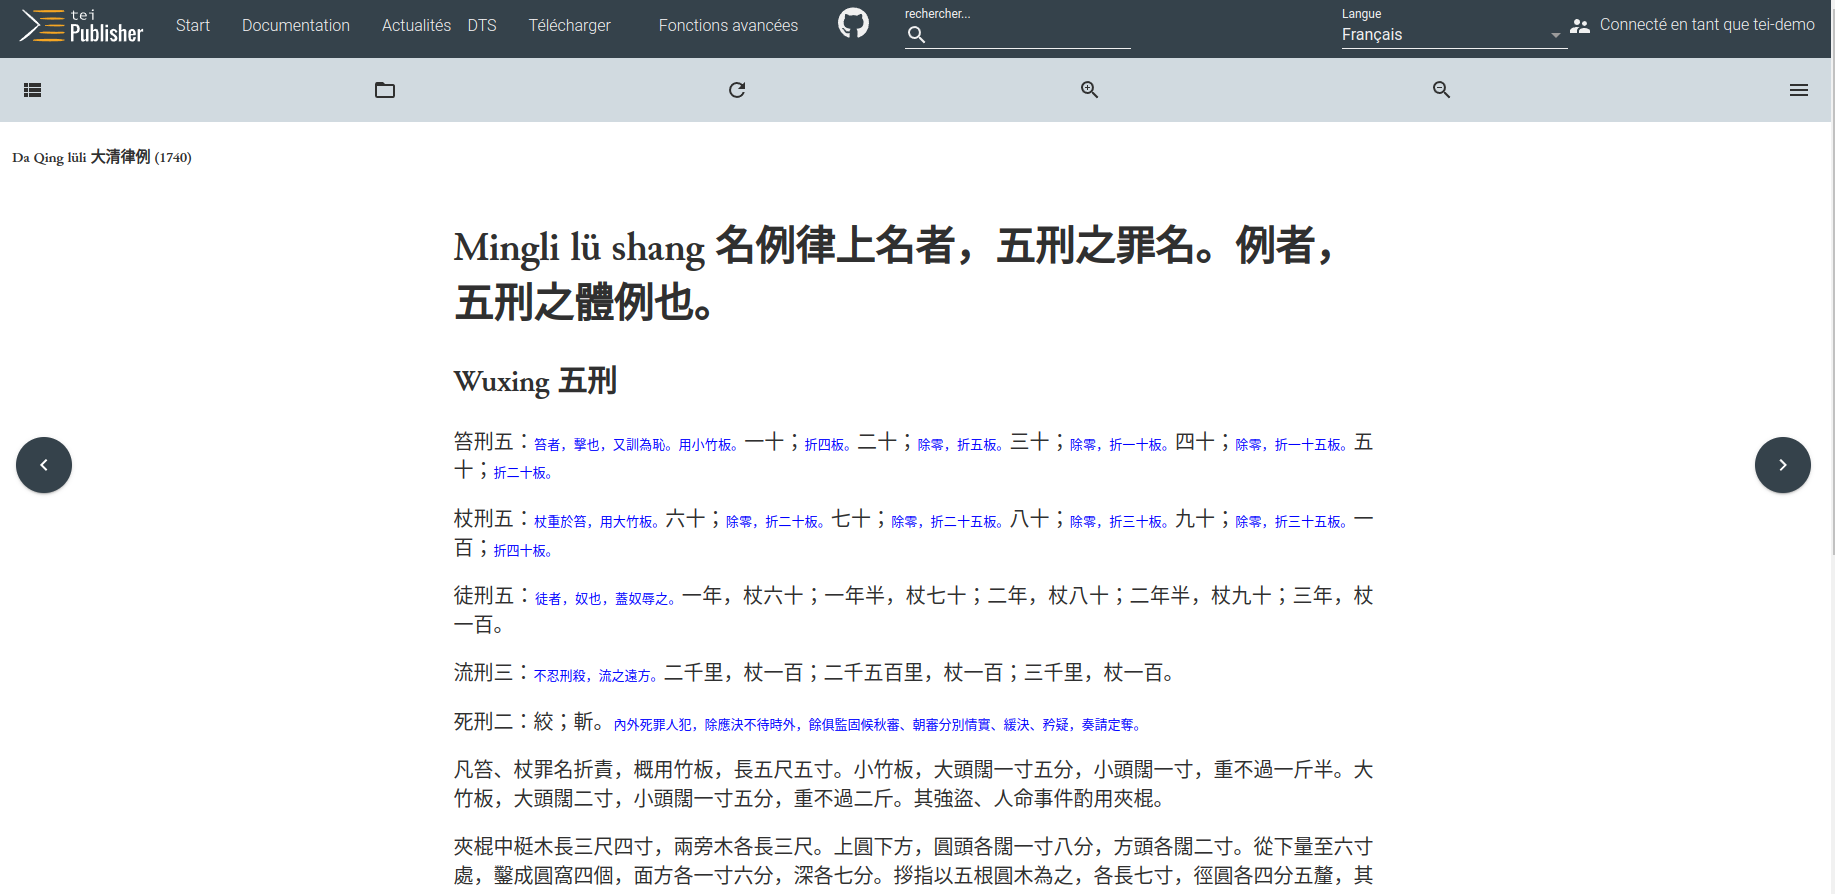
\includegraphics[width=\textwidth]{images/tei_publisher_test.png}
    \caption{Capture d'écran du résultat du test de l'aire de jeux}
\end{figure}

Le mode d'affichage principal souhaité par le projet permet de mettre en avant les commentaires officiels contenus par les textes de lois, en caractères bleus de police inférieure au texte principal. Ces commentaires, contenus dans des balises \texttt{<note/>} ont été sélectionnés via un chemin \xpath : \texttt{@type='official'}. En effet, les textes contiennet plusieurs types de commentaires. Seuls les commentaires officiels ont été sélectionnés afin de leur attribuer un comportement. Par défaut, \tp traite les balises \texttt{<note/>} comme des notes de bas de page, via le comportement \textit{note}. Afin de les affichers au sein du texte, il a fallu modifier le comportement par défaut et sélectionner le comportement \textit{inline}, qui permet d'afficher les balises au sein du texte. Ensuite, le code \CSS suivant a permis d'afficher ces commentaires en bleu dans une police inférieure : 

\begin{minted}{css}
    font-size: small; color: blue;
\end{minted}

L'aire de jeux \tp est donc un moyen efficace de tester les fonctionnalités offertes par l'application avant de démarrer un projet. Grâce à la veille informationnelle puis au test effectué lors du stage, il a été possible de déterminer que \tp semble être un outil compatible avec les besoins du projet et la réalisation des livrables. Cependant, il est également possible de souligner les limites de \tp. En effet, bien qu'entièrement réalisable en interface graphique, l'édition scientifique numérique via \tp nécessite une bonne maîtrise des langages \XML et du développement web, notamment \HTML et \CSS. La réalisation d'un site web via \tp permet de passer moins de temps à coder et de créer une édition dans le respect des normes d'interopérabilité et de pérennité des données sur le web. Cependant, la prise en main de l'outil n'est pas instantanée et nécessite des compétences techniques minimales et un temps de formation. Si les chercheurs auront la possibilité d'ajouter et de modifier des documents sans problème en \XML, via l'interface eXist, il leur sera plus difficile de paramétrer les modes d'affichages seuls, malgré l'interface graphique de \tp. 


             
            
        \clearemptydoublepage
        
        \chapter{Assurer un outil pérenne}
                    \section{Le choix de la science ouverte}
    \subsection{Publication des données sous licence libre : la licence Etalab}

Le projet \COREL souhaite produire une édition scientifique numérique \textit{open source} et contribuer à l'enrichissement des données de la recherche. Lors de la rédaction du cahier des charges et de l'établissement d'un jeu de données en \TEI, la question de la licence à utiliser s'est posée. De nombreux projets de recherche utilisent les licences \textit{Creative Commons}, dont le site internet permet de choisir facilement une licence qui correspond aux besoins de chacun. En effet, un questionnaire à remplir permet ensuite de rediriger l'utilisateur vers la licence qui correspond le mieux à ses réponses. Les licences Creative Commons sont également bien documentées afin de permettre à chacun de choisir au mieux la licence qu'il souhaite utiliser. 

Dans un premier temps, la possibilité d'utiliser une licence CC-BY-SA\footnote{https://creativecommons.org/licenses/by-sa/4.0/} a été envisagée par le projet. Cette licence permet d'autoriser la réutilisation des données en attribuant au projet \COREL la paternité des données originales et d'indiquer les modifications effectuées sur les données (BY), et de partager les données dans les mêmes conditions que le projet \COREL, c'est-à-dire en conservant la licence CC-BY-SA. 

Toutefois, le projet \COREL est un projet de recherche public. C'est pourquoi la licence Etalab\footnote{https://www.etalab.gouv.fr/licence-ouverte-open-licence/} a finalement été choisie pour le projet. Mise en place par le gouvernement français dans le cadre de l'\textit{open data}, cette licence est : 

\begin{quote}
    la licence de référence pour les administrations pour la publication de données publiques.\footnote{Ibid.}
\end{quote}

Cette licence est équivalente à la licence CC-BY et est donc compatible avec celle-ci, si le projet \COREL atteint des chercheurs en droit chinois ailleurs que dans le cadre de la réglementation française. Le choix de cette licence s'est imposé afin de respecter la licence mise en place par le gouvernement pour les institutions publiques. La réflexion autour de cette licence a également permis au projet d'envisager des conditions de réutilisation plus libres. En effet, la licence CC-BY-SA présente plus de contraintes que la licence CC-BY ou Etalab, étant donné qu'elle impose aux utilisateurs de repartager les données sous la même licence. La licence CC-BY n'impose aucune restriction et permet de partager ses données en \textit{open access}, sans autre condition que l'attribution de la paternité de l'oeuvre à un tiers. En souhaitant contribuer à l'ouverture des données et au partage des données publiques, le projet \COREL a donc choisi d'utiliser la licence Etalab en France afin de s'inscrire dans une démarche de science ouverte. 

\subsection{Utilisation d’outils open-source, maintenus par une communauté scientifique}

En plus du choix de la licence, il était essentiel pour le projet d'utiliser des outils et langages \textit{open source} et bien documentés, afin d'éviter les écueils des projets précédents. En effet, les données des projets précédents, bien que pensés pour être disponibles en \textit{open access} n'ont en réalité pas contribués à la science ouverte et à l'enrichissement des données de la recherche. Les données du projet \LSC ont été balisées en \XML afin d'utiliser un langage standard de partage des données. Cependant, le manque de documentation et de diffusion de ces données a contribué à l'établissement de données difficiles d'accès et non-réutilisables. Afin de publier des données dans les principes \fair et rétablir l'accès aux sources du droit chinois, le projet \COREL a donc transformé ces données en \TEI, ce qui a permis d'établir un schéma d'encodage bien documenté, qui pourra être consulté par des chercheurs en droit chinois et en humanités numériques. Afin de contribuer à l'ouverture des données, il est également nécessaire de publier ces données afin qu'elles soient accessibles librement sur le web, par exemple sur une page GitHub dédiée au projet.

De plus, la plateforme \tp, maintenue par une communauté scientifique en publication de données \TEI, permet au projet \COREL d'utiliser un outil \textit{open source} et bien documenté. Cela permet d'éviter la création d'une plateforme éphémère comme le site web \LSC, laissé à l'abandon par son propriétaire, sans moyen de l'entretenir. L'usage d'un outil \textit{open source} a pour avantage d'être maintenu par une communauté entière, à l'inverse d'un site propriétaire. De plus, \tp étant fondé sur le \TEI Processing Model, si la plateforme venait à ne plus fonctionner, l'\ODD générée par celle-ci serait toujours utilisable puisqu'elle s'inscrit dans les standards de la \TEI. Néanmoins, l'utilisation d'un outil \textit{open source} n'est pas le seul garant de la maintenabilité du site web du projet dans le temps, même après le financement. Il est essentiel de penser également à cette question de pérennisation des données publiées en ligne, afin de produire une véritable contribution à la science ouverte, et non une plateforme à durée de vie limitée. 

 \section{Perspectives et évolutions du projet }
    \subsection{Maintenance et hébergement}
Afin d'assurer un outil pérenne pour les chercheurs, il est nécessaire de penser en amont à l'hébergement et à la maintenance du site web. Ces deux aspects du projets ont été intégrés au cahier des charges, afin de souligner l'importance d'héberger et de maintenir le site web du projet dans le temps pour ne pas créer une plateforme qui deviendrait obsolète dans quelques années. 

Plusieurs solutions sont envisagées pour l'hébergement. Étant donné que le projet résulte d'une collaboration entre les institutions, il est possible que le \cdf ou l'\EFEO soient, l'un ou l'autre, l'hébergeur du site web. Le projet envisage également de faire appel à Huma-Num pour héberger le site. Huma-Num propose d'héberger gratuitement, cependant la maintenance reste aux frais du projet et doit être garantie afin d'obtenir l'hébergement d'Huma-Num. De plus, d'autres conditions sont spécifiées sur le site web de l'infrastructure\footnote{https://documentation.huma-num.fr/hebergement-web/}, afin d'assurer aux utilisateurs que les données soient ouvertes et interopérables. Les données et métadonnées du site doivent, notamment, être référencées dans Isidore\footnote{Isidore est un moteur de recherche mis en place par Huma-Num pour les sciences humaines et sociales, qui référence des publications scientifiques, colloques et toutes sortes de documents et permet de faire une recherche plein texte dans ces documents.} via le protocole \oai \footnote{Ce protocole permet de garantir l'interopérabilité des données grâce à un standard permettant de diffuser des données et d'en collecter.}. Bien que seul l'hébergement Huma-Num requiert obligatoirement le respect de ce standard, l'interopérabilité et l'ouverture des données sont essentiels pour l'équipe du projet, afin d'enrichir les données de la recherche et de produire un outil accessible aux chercheurs, contrairement au site web précédent qui n'est plus maintenu et ne respecte pas les principes \fair des données. Le référencement dans Isidore fait donc partie des étapes de mise en place du site web, peu importe l'hébergeur choisi. 

Par ailleurs, la maintenance envisagée pour le projet \COREL est essentiellement corrective, afin de garantir un site web pérenne dans le temps. En effet, les chercheurs souhaitent pouvoir mettre à jour le site internet avec de nouveaux documents, sur le même modèle d'encodage défini pour les textes légaux. Si les nouveaux documents \TEI respectent le schéma de validation de l'\ODD, les documents devraient s'afficher correctement grâce à l'\ODD de \tp. Ainsi, le site web du projet ne demande qu'une maintenance corrective, sans ajout de nouvelles fonctionnalités. Cette maintenance sera assurée par Vincent Paillusson et permettra de veiller à la bonne intégration des nouveaux documents sur le site. 

\subsection{Les évolutions envisagées}

L'évolution principale du projet \COREL consiste en l'ajout de nouveaux documents. En effet, des recueils de cas et de jugements sont actuellement en train d'être numérisés par la bibliothèque d'études chinoises. À termes, il est donc envisagé de les intégrer au site internet du projet et de les lier aux lois auxquelles elles sont rattachées. En effet, certains cas donnent naissance à de nouvelles lois ou articles additionnels afin d'adapter la loi à un cas spécifique. Afin d'offrir aux chercheurs un outil permettant d'étudier l'évolution et la généalogie des lois, intégrer ces recueils de cas au site web n'est donc pas sans intérêt pour la recherche. L'ajout de ces nouveaux documents nécessite de les encoder en \TEI sur le même modèle que les textes de lois. Toutefois, le modèle d'encodage ayant été créés pour les codes légaux sans prendre en compte les recueils de cas, le schéma d'encodage devra vraisemblablement être adapté aux nouveaux documents et nécessitera de modifier l'\ODD de \tp ou d'en créer une nouvelle afin de personnaliser l'affichage pour ces documents. Ces évolutions relèvent donc de la maintenance évolutive étant donné que le paramétrage de l'application réalisée avec \tp devra être modifié afin de s'adapter à ces nouveaux ajouts. 

De plus, l'ajout d'autres visualisations ont été évoquées pendant le stage, mais n'ont pas été intégrées au cahier des charges car elles outrepasse le périmètre du projet. Il est toutefois intéressant de conserver ces perspectives d'évolution du projet. Ainsi, les visualisations suivantes peuvent être envisagées comme une évolution du site web du projet : 

\begin{itemize}
    \item Établir une cartographie du code : l'organisation d'un code légal a pu changer dans le temps et certaines lois additionnelles peuvent changer de \lu de rattachement. 
    \item Réaliser des études statistiques sur les textes : le pourcentage de caractères ayant changé d'une version à une autre d'un code légal ou suivre des évolutions de vocabulaire par exemple.
\end{itemize}

Le projet \COREL envisage donc une maintenance corrective afin de maintenir le site web dans le temps et permettre aux chercheurs d'accéder aux données et à l'édition des textes librement. Toutefois, des évolutions plus importantes sont également pensées et nécessiteraient une maintenance évolutive, et probablement un financement supplémentaire afin de les mener à bien. Bien que ces perspectives d'évolution soient hors périmètre dans le cadre du projet, il est important de les envisager en amont afin de fournir aux utilisateurs un site web pérenne et des données utilisables, qui respectent les principes de l'\textit{open data} et soient consultables et réutilisables par les chercheurs et ainsi produire une plateforme utile à la recherche. 


             
            
        \clearemptydoublepage
    
    \chapterNo{Conclusion}
    \pagestyle{empty}
    \addcontentsline{toc}{chapter}{Conclusion}

\appendix
    \part*{Annexes}	
    \addcontentsline{toc}{part}{Annexes}
    \pagestyle{empty}
    \chapterNo{Annexe A - Cahier des charges}
Ce cahier des charges a pour objectif de présenter le projet \COREL et d’en définir précisément les besoins et objectifs. Il contient un état des lieux des outils et sources, ainsi qu’une description des livrables attendus. Quelques préconisations techniques pour répondre à ces objectifs sont faites en fin de document.

\section*{Les enjeux}
Le projet \COREL fait l’objet d’un financement \CollEx Persée jusqu’au mois d’octobre 2024 et doit créer, durant cette période, un outil qui répond aux besoins des chercheurs. Cet outil devra être créé à partir d’un corpus vaste, dont les données sont issues de plusieurs sources \footnote{À ce sujet, voir la présentation du corpus.} et hétérogènes (existantes au format \XML, \csv, etc. \footnote{À ce sujet, voir l’état des lieux.}), afin de proposer aux chercheurs une architecture qui agrège les différents outils mis au service du projet, réutilisable par la communauté scientifique. 

De plus, le projet s’inscrit dans un champ disciplinaire particulier, la sinologie et l’histoire du droit. Les outils utilisés devront permettre, dans cette perspective scientifique, de montrer comment évolue le droit. 
\newpage
\section*{Contextualisation du projet}
\subsection*{Le projet \COREL}
Le projet \href{https://www-test-collex.inist.fr/projet/corel/}{\COREL} a pour but la reconstitution de la législation de la Chine impériale tardive à partir de différents corpus : des documents conservés dans les fonds du porteur de la filière IST (\cdf) et sur le travail accompli dans le cadre de programmes de recherche antérieurs (\LSC, \EPJ). Ce projet est un moyen de préserver et de valoriser ce corpus de recherche sur l’histoire juridique, en proposant une édition en ligne des textes de loi sous la dynastie Qing et un accès facilité aux documents sources via un site internet. La recherche sera également facilitée pour les chercheurs grâce à un \textit{code virtuel} \footnote{La notion de “code virtuel” renvoie à un texte de loi reconstitué artificiellement grâce aux différentes versions du code publiées entre 1644 et 1911. Une définition plus approfondie en est donnée dans les livrables du projet. } qui retracera, année après année, l’évolution du droit de 1644 à 1911. 

\subsection*{Projets précédents}
\subsubsection{Legalizing Space in China (\LSC)}
Le projet de recherche Legalizing Space in China (\LSC, financement \ANR 2011-2015) a permis d’inventorier et de collecter l’essentiel du corpus de documents juridiques chinois dont dispose le projet \COREL. Le site internet \LSC propose une version texte des sources ainsi que des documents \pdf. Il dispose également d’un glossaire et de traductions partielles des textes de lois, en anglais et en français.

\subsubsection{Emerging Procedural Justice (\EPJ)}
Le projet Emerging Procedural Justice (\EPJ, financement Arqus/European Alliance pour l’année 2020), en collaboration avec Data Futures, a permis de développer une base relationnelle d’images sur serveur \IIIF associant deux éditions du code des lois de la dynastie Qing (\dq et  l'édition de 1870) et deux compilations décrivant de façon exhaustive l’évolution des lois (\genyuan et \huidian).

\newpage
\section*{Les acteurs}
\subsection*{L'équipe}
\begin{itemize}
    \item Frédéric Constant
    \item Vincent Paillusson
    \item Luca Gabbiani
\end{itemize}

    L’équipe collabore avec le prestataire, Data Futures, ainsi qu’Huma-Num qui héberge et maintient la base de données du projet \LSC.
\subsection*{Les acteurs institutionnels}
La \href{https://www.college-de-france.fr/fr/bibliotheque-archives/bibliotheque-etudes-chinoises}{bibliothèque d’études chinoises} du \href{https://www.college-de-france.fr/fr}{Collège de France} met à la disposition du projet les documents sources sur lesquels s’appuie le projet. C’est le porteur administratif du projet. Le Centre de hautes études chinoises (anciennement Institut des hautes études chinoises) est rattaché au Collège de France et abrite la bibliothèque d'études chinoises, fondée en 1927 par Paul Pelliot et Marcel Granet. Celle-ci dispose d’une des plus importantes collections sinologiques d’Europe. Les fonds atteignent 150 000 volumes. Elle est spécialisée dans les recherches sur la sinologie classique (pré-1912) et conserve de nombreuses monographies locales anciennes (difangzhi 地方志), des collectanea (congshu 叢書, 1 400 titres) ainsi que des manuscrits rares. Elle possède aussi plusieurs éditions originales d’ouvrages utilisés dans le cadre du présent projet, dont certains exemplaires uniques au monde. La bibliothèque a reçu en mai 2021 le label \CollEx.

L’\href{https://www.efeo.fr/index.php}{École Française d’Extrême-Orient} (\EFEO) et l’Université de Nice sont chargés de l’exploitation scientifique du projet. 

L’\EFEO fondée en 1900 à Saigon, a pour mission la recherche interdisciplinaire sur les civilisations asiatiques, de l'Inde au Japon. L'\EFEO est présente, grâce à ses 18 centres de recherche, dans 12 pays d'Asie. Cette spécificité permet à ses 42 chercheurs permanents (anthropologues, archéologues, linguistes, historiens, philologues, sociologues des religions, etc.) d'être sur les terrains de leurs études, et d'animer un réseau de coopérations locales et d'échanges internationaux entre scientifiques orientalistes. L’\EFEO apporte les compétences techniques nécessaires à la réalisation du projet. 

Par l’excellence des établissements de recherche qui la composent et son potentiel d’innovation, \href{https://univ-cotedazur.fr/recherche-innovation}{Université Côte d’Azur} s’inscrit dans une politique de site ambitieuse. CNRS, INRIA, INSERM, INRAe, IRD… les instituts de Recherche nationaux constituent le socle solide d’une recherche pleinement intégrée à l’écosystème universitaire. La recherche s’exerce au travers de plus de 50 Unités Mixtes de Recherche et laboratoires. Plus de 1 200 chercheurs engagés dans des activités de Recherche fondamentale et appliquée sont impliqués dans des réseaux nationaux et internationaux. Ils sont également des acteurs majeurs dans le développement de l’innovation et le soutien de l’économie sur le territoire azuréen.

\subsection*{Prestataires}
\href{https://www.data-futures.org/}{Data Futures GmbH} est une entreprise à but non lucratif située à Leipzig et travaille sur les technologies de redistribution et de préservation des données de recherche ainsi que sur les infrastructures associées. Le partenariat Hasdai entre des institutions européennes et américaines est géré par Data Futures GmbH et est régi par un accord avec le CERN. Hasdai a étendu la technologie du dépôt Invenio du CERN aux sciences de la vie, aux sciences sociales et aux sciences humaines. Il exploite également un réseau de dépôts et d'archives InvenioRDM au nom de ses partenaires. Invenio constitue la base technique de Zenodo, le dépôt universel pour les données de la recherche, soutenu par le CERN au nom de OpenAIRE.

L’\href{https://www.huma-num.fr/quest-ce-que-l-ir-huma-num/}{IR* Huma-Num} a pour mission principale de construire, avec les communautés et à partir d’un \href{https://www.huma-num.fr/conseils-et-comites/}{pilotage scientifique}, une infrastructure numérique de niveau international (nœud français des ERIC \href{https://www.huma-num.fr/infrastructures-europeennes/#dariah}{DARIAH} et \href{https://www.huma-num.fr/infrastructures-europeennes/#clarin}{CLARIN}) pour les SHS. 

Elle structure, par l’intermédiaire de \href{https://www.huma-num.fr/les-consortiums-hn/}{consortiums} regroupant des acteurs des communautés scientifiques et d’un \href{https://www.huma-num.fr/trouver-son-relais-msh/}{réseau de points de présence dans les maisons des sciences de l’Homme (MSH)}, l’accompagnement des communautés scientifiques SHS en matière d’infrastructure numérique pour les données de la recherche. 

Elle met en œuvre une infrastructure numérique permettant aux communautés SHS de développer, de réaliser et de préserver sur le long terme les programmes de recherche – leurs données et outils- dans un contexte de science ouverte et de partage des données. 

L’ensemble de l’infrastructure s’inscrit dans le cadre des principes dits \fair (Facile à trouver, Accessible, Interopérable, Réutilisable) qui favorisent, outre l’ouverture des données, leur mise à disposition avec un triple objectif de qualité des données et des métadonnées, d’inscription dans un cycle de vie maitrisé par les scientifiques et enfin de pérennité des données sur le long terme (accès, intégrité, contextualisation de la production des données). 

Huma-Num IR* est une infrastructure de recherche « étoile », du Ministère de l’enseignement supérieur et de la recherche, mise en œuvre par le CNRS avec le Campus Condorcet et Aix-Marseille université. 

Elle est, avec son entrepôt de données NAKALA, l’un des Centres de référence de l’écosystème national Recherche Data Gouv. Engagée dans l’European Open Science Cloud, elle porte la participation de la France dans l’European Research Infrastructure Consortium (ERIC) DARIAH.
\newpage

\section*{Les objectifs}
Le projet \COREL dispose de plusieurs objectifs. Le premier est de diffuser en ligne un corpus de textes de lois de la Chine Impériale. Ce corpus sera publié sur un site internet créé pour le projet et mis à la disposition des chercheurs en droit chinois. L’objectif est de le rendre exploitable par les utilisateurs, c’est-à-dire que les textes seront consultables et recherchables. 

Cet objectif en entraîne un deuxième, qui est la reconstitution de l’évolution de la législation sous la dynastie Qing. Les sources seront regroupées sur un seul site internet, ce qui en facilitera l’accès. Grâce à ce corpus, la publication de visualisations et la génération d’un \og code virtuel\fg, c’est-à-dire un texte de loi qui reconstitue artificiellement un code légal pour une année donnée, permettra d’étudier l’évolution de la législation, année après année. 

Le troisième objectif du projet est de fournir aux porteurs du projet un site internet pérenne, qui sera modifiable, notamment pour en enrichir le contenu, en interface graphique.
\newpage
\section*{Les évolutions possibles}
L’un des objectifs du projet est de créer un site internet qui pourra évoluer avec le temps. Le projet \COREL possède en effet des perspectives d’enrichissement, notamment l’intégration de sources sur les jugements, les cas et les peines. Ces documents sont en cours de numérisation par la bibliothèque d’études chinoises du Collège de France. 

Ces documents seront directement liés au corpus : il ne s’agit pas simplement d’ajouter de nouveaux documents, mais de permettre aux chercheurs de mettre ces documents en relation. Certains cas ou jugements donnent naissance à des lois et il serait intéressant de pouvoir lier ces textes aux lois. 

De plus, un dépôt des images résultant de la numérisation du code est envisagé sur \href{https://www.nakala.fr/about}{Nakala}. 

\newpage
\section*{Les contraintes}
Le projet \COREL possède un financement limité dans le temps, jusqu’au mois d’octobre 2024 et devra donc être réalisé dans le temps imparti. De plus, les données mises à notre disposition sont hétérogènes : données \XML, exports de Freizo (\csv, \JSON), etc. \footnote{Voir l’état des lieux. }

Le projet s’appuie sur des projets précédents et cherche donc à s’inscrire dans la continuité de ceux-ci. Pour cela, la reproduction partielle du site Legalizing Space in China est envisagée. \footnote{Voir les maquettes et la partie édition en ligne.}

Ce projet d’humanités numériques doit de plus garantir la maintenabilité des livrables dans le temps, en utilisant des outils open-source et bien documentés. Ces outils devront être accessibles en interface graphique aux chercheurs qui n’ont pas de compétences techniques et devront être choisis pour leur flexibilité, afin de laisser ouverte la possibilité d’une évolution du projet dans le temps. 

Le projet ne souhaite pas créer un site web via un développement customisé et souhaite utiliser un outil accessible et exploitable librement, avec une documentation disponible en ligne, et une communauté d’utilisateurs bien développée. Cet outil devra permettre de diffuser les textes de lois en ligne, personnaliser l’affichage et pouvoir ajouter des pages au site internet avec un système de gestion de contenu, sans nécessité de coder. L’ajout, la suppression ou la modification des pages doit être accessible en interface graphique. Cet outil doit aussi intégrer un système de gestion de base de données \XML pour pouvoir gérer la base de données du projet et l’enrichir. L’outil utilisé pour le projet doit être open-source et ne doit pas dépendre d’un tiers, que ce soit pour le développement ou la maintenance (qu’elle soit corrective ou évolutive).

\newpage
\section*{Présentation du corpus}
La bureaucratie chinoise de l’époque impériale rendait la justice en application de codes promulgués en général en début de dynastie et régulièrement mis à jour. La première édition du code publiée sous la dynastie Qing date de 1646 et contient plusieurs centaines d’articles ; la dernière, promulguée en 1870, en regroupe environ 2000. Si l’on ajoute les dispositions entre temps abrogées ou modifiées, la législation Qing a compris plusieurs milliers d’articles. Par ailleurs, le droit chinois évoluait lorsque des édits élevaient au rang de loi des décisions rendues dans des affaires importantes ou à la suite de mémoires proposant une modification du droit. La relation entre les lois et les jugements n’était pas univoque et il existait une dynamique complexe entre les deux sources.

Une révision du code est faite environ tous les 10 ans, il existe 23 éditions successives des codes chinois mais seulement une partie a été conservée. Notre corpus est constitué de quatre éditions sur la période 1644-1911.
Un premier texte de loi a été publié en 1646. Le deuxième est paru en 1740. Ce code fixe les \lu, les lois principales, de manière définitive. Elles ne sont plus modifiées ensuite. Ces codes comprennent aussi les \li, des lois secondaires qui font partie du droit vivant. Les \lu se réduisent au fur et à mesure, tandis que les \li augmentent. Les codes sont divisés en 7 chapitres, dans lesquels se trouvent les sections, les lois principales, puis les lois secondaires. La division en chapitres correspond aux différents ministères.

Le \textit{Da Qing lüli genyuan 大清律例根源} présente les lois additionnelles organisées de manière chronologique, donc dans l’ordre de modification du code. 
Le \textit{Huidian shili 會典事例} est un texte de 1899 qui compile l’ensemble des lois en vigueur ainsi que les textes abrogés. Il organise les lois en classant les \li selon la loi principale à laquelle elles sont rattachées.

Le \textit{Duli cunyi 讀例存疑} est un texte de 1906, qui compile les lois en vigueur sous la dynastie Qing avec des explications historiques. Il a été établi par Xue Yuncheng pour aider à la révision du code des Qing.

Ces quatre sources permettent de reconstituer la législation chinoise entre 1644 et 1911, mais cela nécessite de croiser les informations. Certaines lois sont présentes dans plusieurs ouvrages, tandis que d’autres n’ont été retranscrites que dans un seul. Il est donc nécessaire de croiser les sources. 

\newpage
\section*{L'état des lieux}
\subsection*{Les documents \XML}
\subsubsection{L’encodage XML}

Les documents sources ont été océrisés puis encodés en \XML, selon un schéma propre au site internet \LSC. La structure des textes de lois chinois (chapitres, sections, lois principales et lois secondaires) est conservée dans le balisage. 

Les documents sont conçus sur un modèle d’encodage trilingue. Chaque balise est donc répétée avec un attribut de langue différent (chinois, anglais ou français), cependant la traduction n’est pas systématique, laissant certaines balises vides. 

De nombreuses pièces liminaires (par exemple \texttt{<description>}, \texttt{<edition>}...) sont présentes pour documenter le projet d’édition \LSC ou présentent du contenu additionnel aux codes légaux. Ces éléments n’ont pas été repris dans le projet \COREL, à l’exception des tableaux synoptiques qui apparaissent au début du code de 1740. Ils donnent une vue d’ensemble sur des catégories transversales, par exemple le montant à verser pour racheter une peine. 

L’encodage \XML est lié à l’affichage du site internet \LSC. Certaines balises \HTML sont utilisées dans l’encodage \XML, par exemple des balises \texttt{<i>}, qui affichent le texte en italique. Les balises \texttt{<inf>}, créées pour le projet \LSC, permettent d’afficher le texte en caractères plus petits, en bleu. 

\subsubsection{La transformation en XML-TEI}
\textbf{Pourquoi la TEI ? }

La \TEI (\href{https://tei-c.org/}{Text Encoding Initiative}) propose un standard d'encodage préconisé pour l'édition scientifique. Elle est largement utilisée dans le domaine de la recherche et offre une documentation en ligne complète. La \TEI permet d'encoder les textes de manière sémantique en distinguant la forme (l'affichage) du fond (le contenu intellectuel). L'encodage en \XML-\TEI assure également l'interopérabilité des données, favorisant l'échange et la collaboration entre les projets de recherche.
Les documents \XML encodés pour le site \LSC ont été transformés via une feuille de style \XSL en \XML-\TEI. Cette transformation a été motivée par deux objectifs : utiliser un balisage sémantique, contrairement au balisage \XML original qui était lié à l’affichage du site internet, pour structurer les documents, et se conformer à un langage universel, préconisé pour l’édition scientifique. Son utilisation s’insère dans une culture métier et scientifique déjà fortement impactée par son usage. De plus, le choix de balises du schéma \LSC devenait trop restreint pour un balisage sémantique (une liste de balises restreinte était prise en compte sur le site internet). Le passage à la \TEI permet de choisir des balises plus adaptées à chaque élément des sources.

Cette transformation a permis d’établir un \href{https://sharedocs.huma-num.fr/wl/?id=yHHcUPKWyusazIZqWVLgtbZI7J65OaLA&path=TEI%282%29&mode=grid}{jeu de données de référence} : la conversion en \TEI reprend toutes les informations nécessaires au projet \COREL présents dans les documents \XML à l’heure actuelle. Ce jeu de données est encore partiel : il manque certaines données dans les documents \XML qui devront être récupérées afin de les intégrer à l’encodage \TEI.
\bigskip
\textbf{Choix d’encodage}
Les documents \XML ayant été encodés pour le projet précédent (\LSC), toutes les données ne sont pas pertinentes pour le projet \COREL. Seuls les éléments structurants des documents ont été conservés et transformés en balises \TEI. C’est le cas des chapitres (\textit{bu}), sections (\textit{men}), lois principales (\textit{lü}) et lois secondaires (\textit{li}). 

Le passage à la \TEI a également permis de sémantiser certaines balises \XML qui étaient liées à l’affichage sur le site internet \LSC, notamment les balises \texttt{<inf>} qui sont des commentaires officiels du code. Un \href{https://sharedocs.huma-num.fr/wl/?id=yHHcUPKWyusazIZqWVLgtbZI7J65OaLA&path=ODD&mode=grid}{guide d’encodage} a été rédigé pour ces documents. 

Les documents \TEI sont constitués d’un \texttt{<teiHeader>} qui contient les métadonnées relatives aux documents sources et à l’édition en ligne. 

\noindent 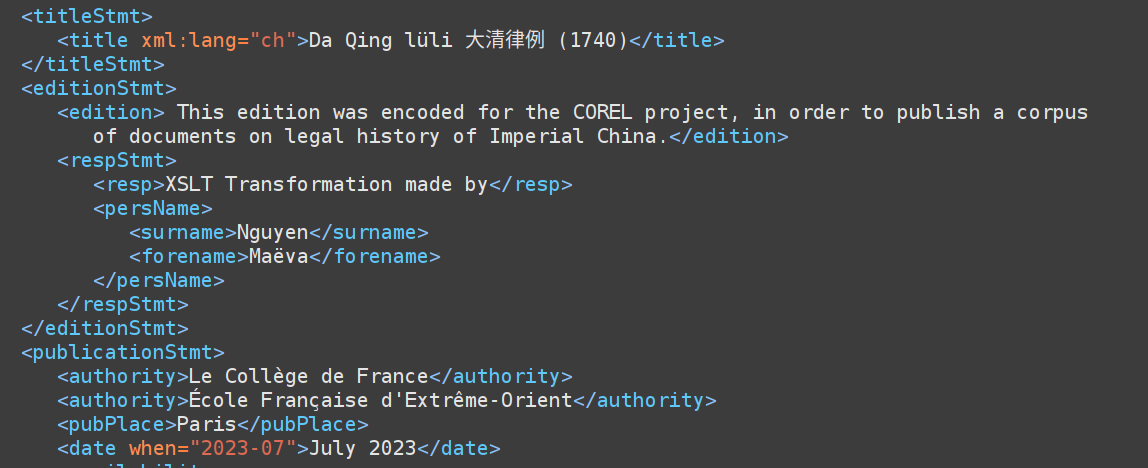
\includegraphics[width=\textwidth]{images/annexe1.png}

Chaque document est contenu dans une balise \texttt{<text>} avec deux attributs : un attribut de langue (le chinois) et un identifiant unique qui permet d’identifier le code légal. 

\noindent 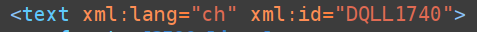
\includegraphics[width=\textwidth]{images/annexe2.png}

Les chapitres, sections et lois sont contenues dans des balises \texttt{<div> }imbriquées. Ces balises ont obligatoirement un attribut \texttt{@type} et une numérotation. Elles sont immédiatement suivies d’une balise autofermante \texttt{<pb/>}.

\noindent 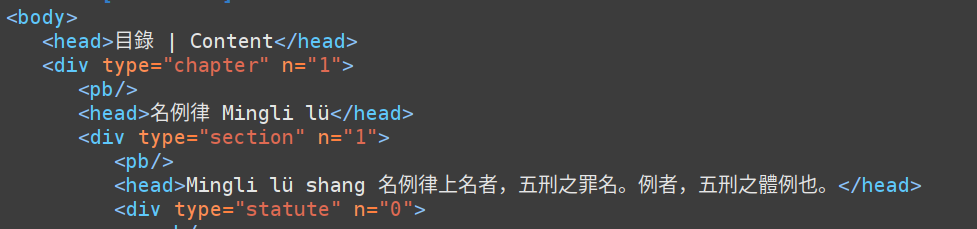
\includegraphics[width=\textwidth]{images/annexe3.png}

Les commentaires contenus dans le code légal sont marqués par une balise \texttt{<note>} dont l’attribut \texttt{@type} est \og official \fg. 

\noindent 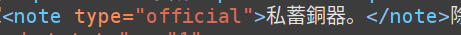
\includegraphics[width=\textwidth]{images/annexe4.png}

Le \huidian contient également des listes qui sont balisées comme suit. Chaque élément de la liste (\texttt{<item>}) contient une date et un ou plusieurs paragraphes. 

\noindent 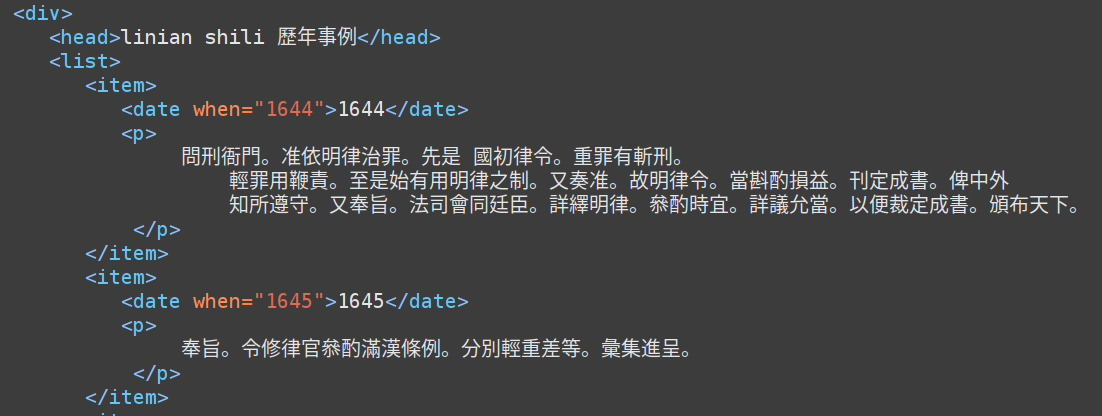
\includegraphics[width=\textwidth]{images/annexe5.png}

Les entités nommées au sein du texte ont été marquées par des balises \texttt{<persName>} pour les noms de personnes, \texttt{<placeName>} pour les noms de lieux et \texttt{<bibl>} pour les références bibliographiques. 

\subsection*{Les métadonnées \IIIF}
\subsubsection{Serveur \IIIF et annotations}

La numérisation des codes légaux a été mise en ligne via la plateforme Freizo, sur un serveur \IIIF. \IIIF (International Image Interoperability Framework) est un protocole qui permet la diffusion et l’échange d’images en haute définition sur le web. La plateforme Freizo donne accès à ces images via le visualiseur Mirador, qui offre la possibilité d’annoter les images et de les segmenter. Les annotations se font sur l’interface web dédiée et sont accessibles et modifiables en interface graphique, ainsi que via des fichiers \JSON. Cette méthode d’annotation permet aux chercheurs de relier de façon précise les métadonnées à des segments de texte. Cette partie du travail a été réalisée par Data Futures \footnote{Pour Data Futures, voir les acteurs, section ‘prestataire’.} lors du projet \EPJ \footnote{Concernant le projet EPJ, voir la contextualisation du projet.}. Les annotations permettent de déterminer le commencement d’un chapitre, une section ou une loi sur la numérisation. 

Les annotations contiennent les informations suivantes, dans cet ordre : 
\begin{itemize}
    \item   Type : le type du passage segmenté (chapitre, section, lü, tiaoli)
    \item Title (zh) : le titre en caractères chinois
    \item Title (zh-Latn) : le titre en alphabet romain
    \item Substatute : le numéro du tiaoli correspondant
    \item Related (h) : le numéro de la loi dans le Huidian Shili
    \item  Related (d) : Dulicunyi (code de 1871)
    \item  Related (c) : Code de 1740
    \item  Related (g) : le numéro de la loi dans le Genyuan
    \item Ghost : Lorsqu’une version postérieure de la loi est mentionnée dans le commentaire, sans que le texte n’apparaisse. 
    \item Date : la date de début de la loi
\end{itemize}

\subsubsection{Les métadonnées}
Les \href{https://duli-cunyi.freizo.org/browse.cgi}{métadonnées} des images \IIIF sont accessibles via Freizo. Elles contiennent le numéro d’asset (un identifiant unique attribué à chaque fichier), le titre du fichier, le titre du code (pour l’exemple ci-dessous : \textit{Huidian}), et des métadonnées (titre, auteur, producteur, date de création, etc.). Un lien hypertexte permet d’accéder au fichier sous format \PDF. 

\noindent 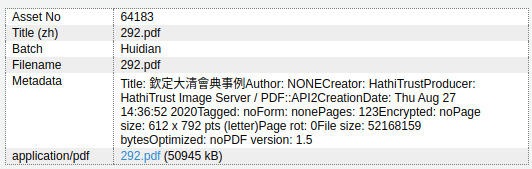
\includegraphics[width=\textwidth]{images/annexe6.png}

\subsection*{Les liens entre les lois}
Sur Freizo des liens entre les lois des différents codes ont été établis. Certaines lois sont présentes dans plusieurs codes, tandis que d’autres ne se retrouvent que dans un seul code. \footnote{À ce sujet, voir la présentation du corpus.} Il existe deux types de liens entre les lois.

\subsubsection{Des liens d'association}
Le premier lien indique les correspondances entre les lois des différents codes. Ce lien est établi à partir du \genyuan et est retranscrit ainsi : \og related duli-cunyi 1 \fg. Cela permet de donner le titre du code et le numéro de la loi correspondant à celle du \genyuan. Il contient également un lien hypertexte qui renvoie à la numérisation, via le visualiseur Mirador. 

\noindent 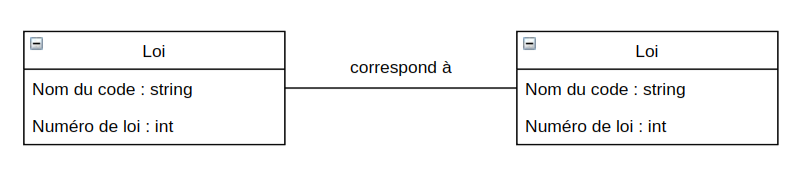
\includegraphics[width=\textwidth]{images/image4.png}

\subsubsection{Des liens d'association dirigée}
Le deuxième type de lien renvoie à des liens de filiation ou d'évolution entre les textes de loi au cours de la période étudiée. Ces relations sont qualifiées de \og \textit{in} \fg ou \og \textit{out} \fg comme ceci : 
 \og genyuan 1-35,o \fg. Le \textit{o} signale une relation \textit{out}, c’est-à-dire que la loi dont on parle prend fin et donne naissance à la loi 1-35 référencée dans le \genyuan. \og genyuan 1-10,i \fg signale une relation \textit{in}, c’est-à-dire que la loi dont il est question est issue de la loi 1-10 recensée dans le \genyuan. 

 \noindent 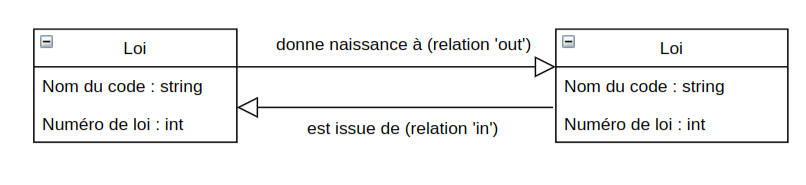
\includegraphics[width=\textwidth]{images/image5.png}

 Ces données ont été exportées au format \csv et/ou \tsv. Un \href{https://sharedocs.huma-num.fr/wl/?id=yHHcUPKWyusazIZqWVLgtbZI7J65OaLA&path=Export_Freizo%2Fgenyuan%20test.xlsx&mode=grid}{premier tableau} contient : 
 \begin{itemize}
     \item le numéro d’asset : un identifiant unique attribué à chaque fichier
    \item  le numéro de page
    \item  une URL qu’il est possible de reconstituer en faisant précéder celle-ci : 
    
    \small \texttt{https://www.google.com/urlq=https://dulicunyi.freizo.org/mirador/ \\book.cgicatno\%3D28941\%26canvas\%D\&sa=D\&source=docs\&ust=1685005327813312\&usg= \\ AOvVaw2BH\_xnL-xkCyTTj4QaCgEy} 
    et en modifiant le numéro catno pour qu’il corresponde au document recherché.
    \item le level : le type de workflow de Freizo
    \item  le titre en chinois
    \item  l’identifiant ‘related’ qui permet d’établir le lien entre les lois
    \item  la date de début de la loi
    \item  l’identifiant qui permet les relations avec les autres textes de loi
 \end{itemize}

Le \href{https://sharedocs.huma-num.fr/wl/?id=yHHcUPKWyusazIZqWVLgtbZI7J65OaLA&path=Export_Freizo%2Fdc-anno-dump-2002-04-14-v2.xls&mode=grid}{second} contient les informations suivantes : 
\begin{itemize}
    \item ressource : une URL
    \item annotatedBy : le nom de l’auteur de l’annotation
    \item  date : la date de début de la loi
    \item  subtype : le type de loi (statute, substatute)
    \item  huidian : le lien vers le Huidian
    \item  dulicunyi : le lien vers le Duli cunyi
    \item  genyuan : le lien vers le Genyuan
    \item  code\_1740 : le lien vers le code de 1740
    \item  title\_zh : le titre en chinois
    \item  number : l’identifiant Freizo
    \item  origin : des informations sur l’origine de la loi
    \item modifications : type de modification apportée à la loi (abrogation, fusion..)
    \item  correspondance : Correspondance avec un autre corpus
    \item related : le numéro de la loi décrite dans le workflow Mirador 2. Les commentaires peuvent être situés avant ou après la loi, il est donc nécessaire de rattacher le commentaire à un segment de texte.
    \item  centraladmin: décision prise par l’administration centrale. Indique également quelle administration est intervenue.
    \item  officialname : le nom du fonctionnaire 
    \item officialfunction : la fonction occupée par le fonctionnaire
    \item  province : le nom de la province
    \item  localadmin : Administration locale ayant rendu le jugement (information de type géographique)
    \item  partyname : Nom des personnes parties à une affaire
    \item original : référence du document original
\end{itemize}
\newpage

\section*{Les livrables du projet}
Le projet \COREL a pour objectif de produire deux livrables pour octobre 2024 : un site internet qui contient l’édition en ligne des textes ainsi que la recomposition de la législation pour une année donnée. Le projet souhaite produire un \POC (Proof of concept) sur un échantillon de lois afin de démontrer la faisabilité du code virtuel. Ce \POC est l’engagement minimal pris auprès de \CollEx Persée pour le financement du projet. Il consiste à générer le code virtuel sur une petite quantité de données (3 lois représentatives).

Tous les livrables du projet, ainsi que les données produites, seront publiés sous la licence \href{https://www.etalab.gouv.fr/licence-ouverte-open-licence/}{Etalab}.

\subsection*{Le site internet}
\subsubsection{Le public cible}
Le premier public visé est la communauté des sinologues, et plus particulièrement les chercheurs qui étudient l’histoire du droit chinois ou utilisent les sources juridiques pour mener des études en histoire sociale, économique ou politique de la Chine, champs d’investigations pour lesquels ces sources sont devenues un matériau essentiel. Le projet vise à mettre à la disposition de ces chercheurs un outil permettant de consulter de nombreux documents pour le moment difficilement accessibles, et d’explorer aisément des données qui n’ont pas encore fait l’objet d’un inventaire et d’une indexation systématiques. 

\subsubsection{Les besoins utilisateurs}
Le premier besoin des utilisateurs est d’avoir accès à une plateforme qui regroupe les différentes sources du droit chinois. En effet, ces sources sont partielles et se complètent les unes les autres, c’est pourquoi proposer une édition en ligne de ces textes est nécessaire pour les chercheurs. L’édition en ligne devra donc contenir les textes de lois, mais aussi des commentaires non-officiels. 

Le projet vise également à agréger ces sources afin de reconstituer la législation de la Chine impériale année après année. Cela permettrait aux utilisateurs d’avoir un accès direct et immédiat à la reconstitution de la législation de la Chine impériale entre 1644 et 1911. Le site internet doit donc être en mesure d’afficher toutes les lois en vigueur pour une année donnée. 

Les chercheurs qui s'intéressent à l’évolution du droit chinois ont également besoin de pouvoir constater l’évolution du droit sous la dynastie Qing. 

\subsubsection{Les besoins administrateurs}

Le site internet devra être entièrement accessible en interface graphique, y compris pour ses administrateurs, afin de pouvoir ajouter des documents et enrichir le site internet après son déploiement en ligne. Pour cela, le site devra proposer un back-office simple d’utilisation, qui permette de se connecter en tant qu’administrateur et de déposer de nouveaux documents, en \textit{drag and drop} ou en parcourant les fichiers de l’ordinateur. 

Les porteurs du projet ont également besoin d’un site qui soit \textbf{autonome}, c’est-à-dire qu’il doit être le moins possible contraint par un tiers. Le site doit être modifiable dans la durée par les administrateurs, sans validation préalable des documents déposés (les créateurs, propriétaires, hébergeurs, etc. du site internet ne peuvent pas refuser la modification du site par un administrateur). Ce besoin est primordial afin de se défaire de la contrainte que représente actuellement le site \LSC, qui ne peut pas être modifié sans la supervision du propriétaire.

\subsubsection{L'aspect du site web}
La description du site internet ainsi que les maquettes ont été réalisées à partir d’exemples de sites \tp, en prenant en compte les besoins utilisateurs et administrateurs. 

Le site web doit contenir une page d’accueil, une page dédiée au corpus, plusieurs pages pour consulter un à un les documents, une page qui affiche le code virtuel, une page de connexion et une page pour administrer le site en interface graphique (télécharger, supprimer, modifier des documents et ajouter de nouvelles pages au site). \footnote{Pour les maquettes du site internet, voir les annexes. }

\bigskip
\textbf{La page d’accueil}

La page d’accueil contient une barre de navigation, qui reste la même pour toutes les pages. La barre de navigation donne accès à la page d’accueil, le corpus, le code virtuel, un à propos, une barre de recherche simple et à l’onglet de connexion. L’onglet \og about \fg est déroulant et affiche l’accès à : des renseignements sur le projet, l’équipe, les mentions légales et le contact. L’onglet \og corpus \fg est également déroulant et donne accès à la liste des documents directement pour faciliter la circulation d’un texte à un autre.

La page contient également le titre du site et sa présentation. Des images avec des liens hypertexte donnent accès au corpus, au code virtuel, et à la présentation du projet. 

Le \textit{footer} du site est le même pour toutes les pages et contient les logos des différentes institutions du projet, les mentions légales, le plan du site et la page de contact. 

\bigskip
\textbf{Le corpus}

Une page affiche la liste de tous les documents disponibles sur le site internet, avec une présentation générale du corpus. La liste des documents contient un aperçu du fac similé, le titre et les métadonnées de chaque document. Ces items sont cliquables et donnent accès à l’édition en ligne de chaque document.

\bigskip
\textbf{L’édition en ligne des documents}

L’édition en ligne propose plusieurs types d’affichage différents. Le premier est un affichage simple, du texte entier et continu. Il est donc possible d’accéder à un code légal en entier sur la même page. La table des matières est navigable et cliquable. Grâce à des ancres, il est possible de naviguer dans le document. 

Le deuxième affichage propose le texte paginé. Comme \LSC, il affiche le texte en plusieurs pages et sépare les chapitres, sections, \lu et \li. En regard du texte, le visualiseur \IIIF propose le code numérisé. Le visualiseur montre la page du texte correspondant au début du chapitre, de la section ou de la loi.

Il est aussi possible d’accéder uniquement au texte paginé, sans visualiseur \IIIF. 

L’affichage du texte paginé permet aussi de choisir différents modes d’affichage. Un affichage \textit{named entities} propose de mettre en avant les entités nommées balisées dans le texte, par exemple en gras. 

Le mode \textit{metadata} permet d’afficher à côté d’une loi ses métadonnées. Ces métadonnées sont stockées dans les commentaires de type \textit{metadata}.

Le mode \textit{commentaries} permet d’afficher les commentaires en plus du texte, à la suite. Ce mode d’affichage n’inclut pas les commentaires de métadonnées des lois, qui sont à afficher dans un mode différent. 

Pour chaque affichage différent, un accès à la table des matières du document devra être disponible via un onglet flottant et indiquer clairement où l’utilisateur se situe dans l’arborescence du document (avec une fonction \textit{hover} par exemple). Cette table des matières sera cliquable pour faciliter la navigation dans le texte. 

Les métadonnées générales devront également être accessibles via un onglet flottant. 

Les titres des lois devront être cliquables afin d’accéder à la page des visualisations.

\bigskip
\textbf{Le code virtuel}

En entrée, la page du code virtuel propose un paragraphe d’explications (qu’est-ce que ce code virtuel et comment l’utiliser ?). Une barre de saisie permet à l’utilisateur de saisir une date entre 1644 et 1911. 

En sortie, le code virtuel affiche toutes les lois dont les bornes chronologiques comprennent la date donnée en entrée. L’affichage est continu, avec une table des matières cliquable qui permet de se déplacer dans le code. Une fonction d’export au format \pdf est disponible pour télécharger le résultat du code généré. \footnote{Pour en savoir plus sur le code virtuel, voir la section suivante, \og recomposition du code virtuel \fg.}

\newpage
\textbf{Une page de connexion}

La page de connexion offre un formulaire avec un nom d’utilisateur et un mot de passe. Elle permet aux administrateurs du site de se connecter et d’accéder au back-office. 

\bigskip
\textbf{Une page d'ajout de nouveaux documents}

Cette page n’est accessible qu’aux administrateurs une fois connectés. Elle propose d’ajouter de nouveaux documents en \textit{drag and drop} ou en parcourant les fichiers de l’ordinateur. 

Lorsque l’utilisateur est connecté, la barre de navigation affiche un nouvel onglet qui permet d’accéder à la page d’ajout. Pour que le document s’affiche correctement sans modifications des paramètres d’affichage, il doit respecter le schéma d’encodage choisi pour les documents.

\noindent 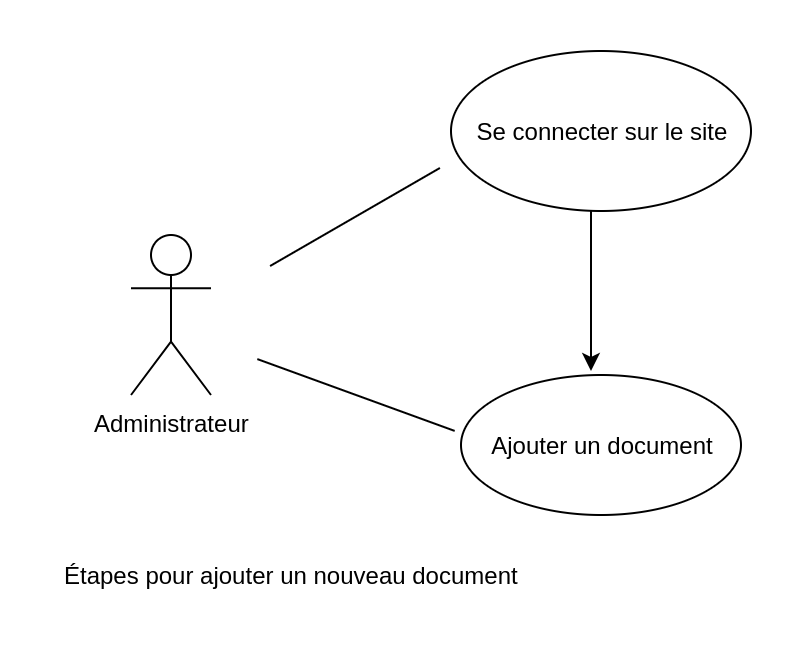
\includegraphics[width=\textwidth]{images/annexe7.png}

Si le site web est réalisé avec \tp, la suppression et la modification de documents déjà mis en ligne se fait via l’interface eXide. L’ajout de nouvelles pages au site internet est possible en encodant les pages souhaitées en \TEI ou en Markdown, ou bien en téléchargeant sur \tp un document .docx. \footnote{Cette fonctionnalité de \tp est encore en cours de développement, mais fonctionne très bien pour éditer des pages simples. Le formatage direct est conservé en grande partie (titre, caractères en gras, etc.) et permet aussi d’intégrer des images. Il y a ensuite la possibilité de personnaliser davantage cet affichage avec l’\ODD de \tp, comme pour l’édition en ligne.}

\bigskip
\textbf{Une page dédiée aux visualisations}

Le site devra proposer des visualisations de ces évolutions, et retracer la généalogie des lois à partir des liens entre les lois. \footnote{À ce propos, voir la modélisation des liens entre les lois.}  La visualisation devra être accessible via l’édition en ligne, en cliquant sur la loi dont on souhaite voir apparaître la généalogie. Pour réaliser ces visualisations, les liens entre les données sur la généalogie des lois sont disponibles dans les fichiers \JSON. 

Les schémas ci-dessous présentent des modélisations simplifiées et non exhaustives de la généalogie possible d’une loi. La visualisation doit retracer toute l’arborescence de la loi et montrer clairement où elle se situe sur l’arbre (modélisé par une couleur différente sur les schémas ci-dessous). La visualisation devra présenter toutes les lois \textit{in} et \textit{out}. 

\newpage
\noindent 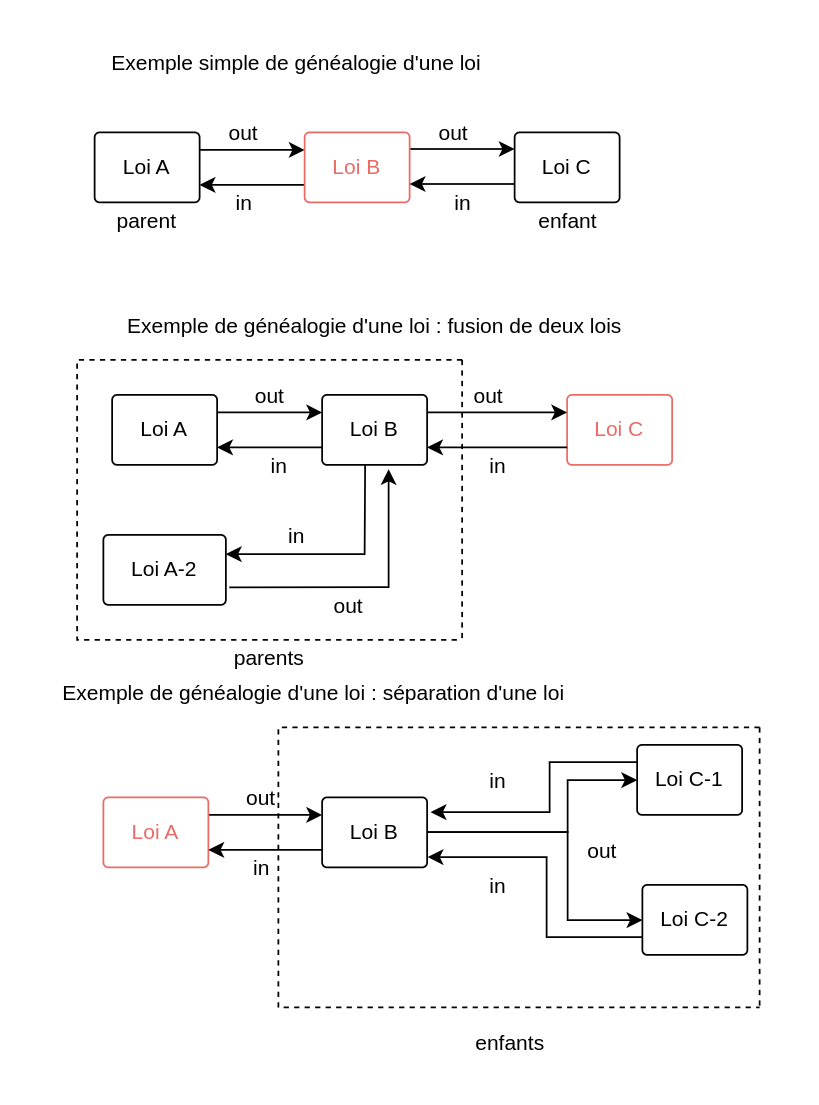
\includegraphics[width=\textwidth]{images/annexe8.png}

\newpage
\subsection*{Recomposition du code virtuel}
Le code virtuel est la recomposition d’un code légal, pour une année donnée entre 1644 et 1911. La recomposition de ce texte de loi présente toutes les lois en vigueur pour l’année choisie, organisées par chapitres et sections. Cette recomposition s’effectue à partir du corpus du projet. 

\subsubsection{Le résultat attendu}
Le code virtuel devra être accessible sur le site en accès libre pour tous les utilisateurs et le résultat doit être accessible rapidement. 

L’utilisateur doit pouvoir entrer l’année de son choix entre 1644 et 1911 et obtenir pour la date choisie une reproduction d’un texte de loi complet qui présente toutes les lois en vigueur pour l’année donnée.

\noindent 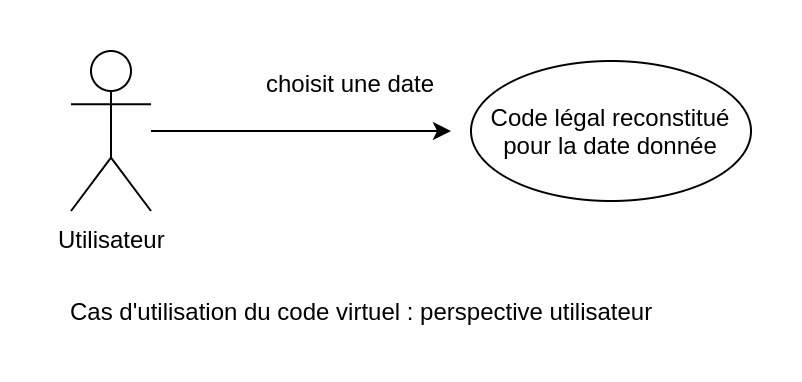
\includegraphics[width=\textwidth]{images/annexe9.png}

Le résultat attendu n’est pas un simple filtrage des lois par date, mais bien une reconstitution artificielle d’un texte de loi. En sortie, le code virtuel doit donc présenter le texte comme s’il avait vraiment été publié, avec un affichage similaire à l’édition en ligne. Il est donc important de conserver la structure du texte de loi (chapitres, sections) et l’ordre des lois (chaque loi secondaire doit figurer sous la loi principale dont elle dépend).

\noindent 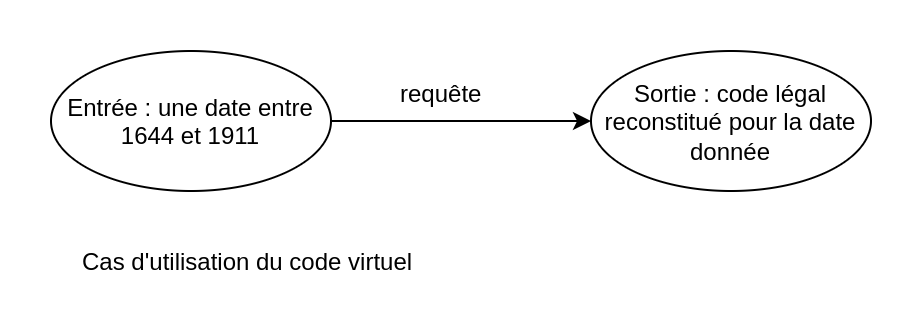
\includegraphics[width=\textwidth]{images/annexe10.png}

\newpage
\section*{Préconisations techniques}
\subsection*{Préparation des données}
\subsubsection{Les données nécessaires}

\textbf{Pour l'édition en ligne}

Pour enrichir les sources afin de répondre aux besoins des chercheurs, les textes de lois doivent notamment être enrichis avec les entités nommées et des commentaires sur les lois (différents des commentaires officiels qui figurent dans les codes légaux). Les entités nommées ont déjà été en partie ajoutées à l’encodage, mais il est pertinent d’ajouter des précisions, notamment des noms de fonction. Ces données sont collectées et accessibles dans les annotations via les fichiers \JSON. 

Pour publier une édition en ligne des codes avec en regard un visualiseur \IIIF, les liens vers les images doivent être intégrés dans l’encodage. Ce lien doit être un accès direct à la ressource. 

Les différents affichages souhaités pour le site sont corrélés à l’encodage des données. Pour afficher les métadonnées d’une loi, il faut intégrer dans les documents, ou dans un document \TEI dédié à cet usage, lesdites métadonnées (avec une référence à l’identifiant \XML de la loi). 

\bigskip
\textbf{Pour le code virtuel}

Pour reconstituer un texte de loi, il faut des bornes chronologiques précises pour chaque loi, afin de pouvoir déterminer quelles lois sont en vigueur pour l’année donnée. Ces données sont disponibles en partie dans les annotations : nous disposons des dates de début de chaque loi. Grâce aux liens d’association dirigée entre les lois, il est possible de déduire la date de fin de chaque loi : une loi prend fin lorsqu’elle est remplacée par une autre. Il faut donc expliciter cette information afin de récupérer pour chaque loi des bornes chronologiques, puis les intégrer à l’encodage. 

Les textes de lois à notre disposition contiennent également des doublons : certaines lois se retrouvent dans plusieurs sources. Il faut donc trouver un moyen de les dédoublonner en leur attribuant un identifiant unique. Cela permettrait de filtrer les lois selon leur identifiant et de n’afficher qu’une seule fois la loi si elle possède des doublons. Les lois qui se retrouvent dans plusieurs codes sont indiquées par les liens d’association entre les lois. \footnote{À propos des liens d’association et d’association dirigée entre les lois, voir l’état des lieux, section \og les liens entre les lois \fg.} Ce système d’identifiant sera également utile pour faire des renvois entre les textes si nécessaire. 

\subsubsection{Échantillon des données}
Un encodage \TEI idéal a été préparé sur un échantillon du \dc (chapitre 6, section 25, \textit{lü} 254 et \textit{tiaoli} 1), afin de présenter ce à quoi les données devront ressembler afin de réaliser le projet. 

\bigskip
\textbf{Les entités nommées}

Pour le balisage des entités nommées, il est recommandé d’utiliser la balise \texttt{<persName>} pour les noms de personne, avec la balise \texttt{<roleName>} si le titre du fonctionnaire est utilisé. 

\noindent 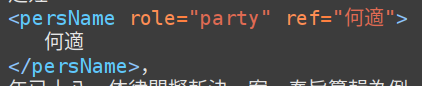
\includegraphics[width=\textwidth]{images/annexe11.png}

Il est également possible de faire dans le \texttt{<teiHeader>} la liste des entités nommées, et de les lister une à une dans la balise \texttt{<person>}. Cela permet de leur attribuer un identifiant unique \texttt{@xml:id} et d’y faire référence dans le corps du texte. Chaque balise \texttt{<person>} contient un attribut \texttt{@role} qui permet de donner le nom de la fonction. Grâce à ce recensement, il est également possible d’ajouter des informations biographiques avec la balise \texttt{<note>}. 

\noindent 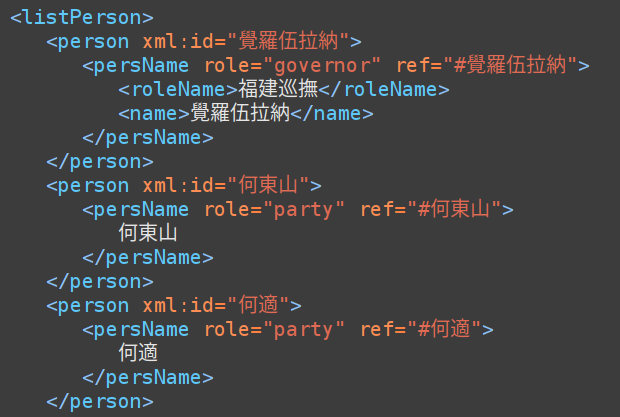
\includegraphics[width=\textwidth]{images/annexe12.png}

Pour les lieux, il est possible d’ajouter un attribut \texttt{@type} (lieu d’application de la loi ou lieu d’origine) et également de faire une liste des lieux, qui contient à minima le nom du lieu et un identifiant unique et éventuellement des informations supplémentaires sur le lieu. Il est également possible de faire correspondre le nom de lieu à l’époque des Qing avec le nom actuel du lieu s’il a changé, de donner des coordonnées géographiques, etc.

\noindent 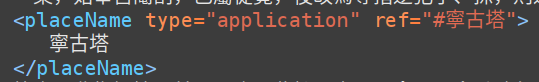
\includegraphics[width=\textwidth]{images/annexe13.png}

Les listes des entités nommées se placent dans le \texttt{<teiHeader>} et contiennent des métadonnées sur ces entités. Cette liste permet aussi d’éviter les erreurs d’encodage car chaque entité nommée est encodée une fois dans le \texttt{<teiHeader>}, puis on se réfère dans l’encodage à l’identifiant \texttt{@xml:id} contenu dans cette liste avec l’attribut \texttt{@ref}. 

\noindent 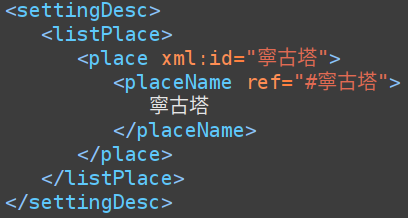
\includegraphics[width=\textwidth]{images/annexe14.png}

\bigskip
\textbf{Les commentaires}

Des commentaires sur les lois peuvent être ajoutés avec la balise \texttt{<note>}. Afin de les distinguer, il convient de leur attribuer un attribut \texttt{@type}. Le nom du type doit correspondre à un mot anglais, par exemple \og official \fg pour les commentaires qui sont rédigés au sein du texte de loi. Les types de commentaires sont déterminés en amont : \textit{official}, \textit{metadata}, etc. Les commentaires de type \textit{metadata} contiennent des métadonnées sur l’origine des lois. 

\bigskip
\textbf{Les liens vers les images}

Afin d’intégrer les images en regard du texte, il est nécessaire d’intégrer le lien de la ressource dans un attribut \texttt{@facs}. Ces liens peuvent se retrouver dans les fichiers \JSON. Le projet n’a pas pour objectif de créer un fac similé interactif, mais simplement de permettre à l’utilisateur de consulter les sources via le visualiseur \IIIF. Les attributs \texttt{@facs} devront donc apparaître sur les balises \texttt{<div>}, la segmentation effectuée permettant d’identifier le début des chapitres, sections et lois. 

\bigskip
\textbf{Les bornes chronologiques}

Afin de pouvoir filtrer pour une année les lois en vigueur, il est nécessaire d’ajouter pour chaque loi une date de début et une date de fin. Pour ajouter les dates en tant qu’attribut sur chaque loi principale et loi secondaire, il est possible d’adapter la \TEI dans l’\ODD afin d’autoriser les attributs \texttt{@notBefore} et \texttt{@notAfter} sur les balises \texttt{<div>}. Les dates sont à récupérer dans les annotations des images.

\bigskip
\textbf{Les identifiants des lois}

Pour pouvoir identifier les lois qui sont présentes dans plusieurs sources, il faudrait un identifiant pour chacune. Une même loi, présente dans plusieurs sources, aurait donc le même identifiant. Il est possible de récupérer cette information via les liens d’association entre les lois qui ont été établis dans Freizo. 

\noindent \includegraphics[width=\textwidth]{images/annexe15.png}

\subsubsection{Étapes de transformation et de validation}
Pour obtenir un document encodé en \TEI à partir des documents \XML du projet \LSC, il est nécessaire de transformer le document \XML grâce à la feuille de style \XSL via le logiciel Oxygen. Les documents doivent ensuite être encodés avec les informations manquantes, en prenant exemple sur l’échantillon. Les données doivent ensuite être validées par l’\ODD, qui contient les règles de validation du schéma choisi pour l’encodage des documents. C’est une étape préalable à l’ajout des documents sur le site. 

Il est également possible d’encoder directement des fichiers en \TEI, auquel cas l’étape de transformation \XSL n’est pas nécessaire. Il suffit d’ajouter les informations aux documents \XML-\TEI de référence, ou bien d’encoder un nouveau document en \TEI en suivant la documentation. 
\newpage
\noindent 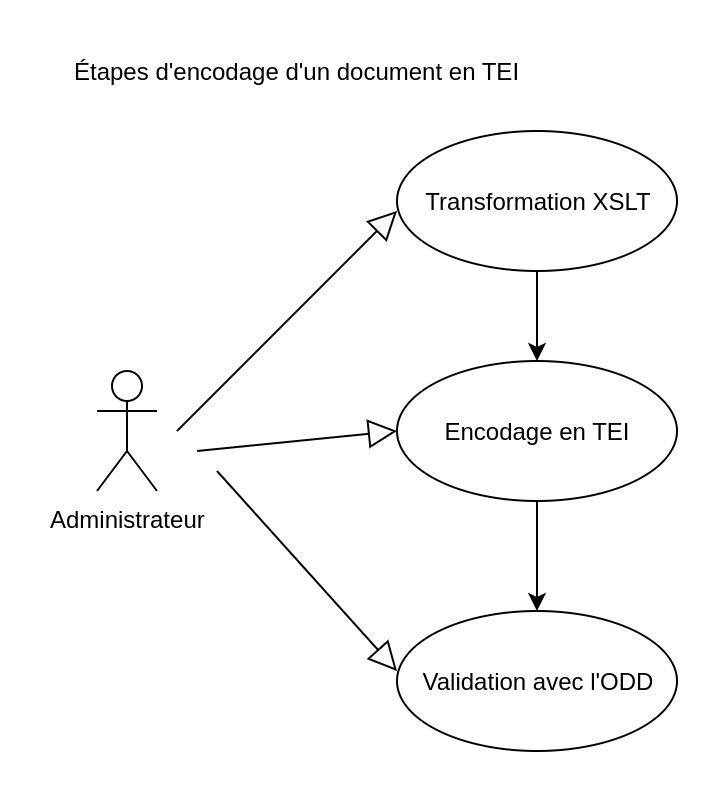
\includegraphics[width=\textwidth]{images/annexe16.png}

Pour valider un document avec l’\ODD, il faut lier le fichier \href{https://sharedocs.huma-num.fr/wl/?id=yHHcUPKWyusazIZqWVLgtbZI7J65OaLA&path=ODD%2Fout&mode=grid}{ODD_COREL.rng} dans le document \TEI, comme ceci : 

\noindent 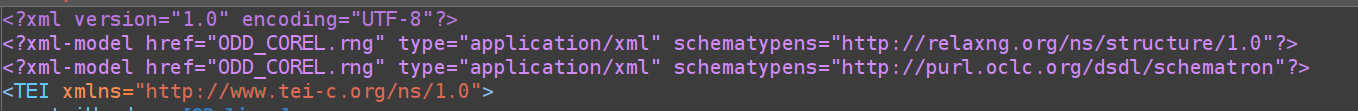
\includegraphics[width=\textwidth]{images/annexe17.png}

L’\ODD permet ensuite à Oxygen de signaler les erreurs à l’utilisateur, avec plusieurs niveaux d’importance. Les erreurs rouges signalent un problème d’encodage bloquant pour le projet, par exemple l’absence de données comme les dates des lois ou les identifiants \texttt{@xml:id}. Les erreurs oranges signalent des erreurs moins importantes, comme par exemple l’absence de l’attribut \texttt{@facs}, qui est nécessaire pour proposer la numérisation des codes sur le site, mais qui n’empêche pas son bon fonctionnement.
\newpage

\section*{Outil envisagé}
\href{https://teipublisher.com/exist/apps/tei-publisher/doc/documentation.xml?odd=docbook&view=div&id=selected-use-cases&hash=3.6.5#introduction}{\tp} est un outil dédié à la publication de textes encodés en \XML-\TEI en ligne. Il s’appuie sur un système de gestion de base de données \XML, eXist-db. L’objectif de \tp est d’offrir un framework permettant de publier des éditions en ligne avec le moins de code possible. Il offre donc une interface graphique qui permet de publier rapidement et simplement des textes, mais permet aussi un grand niveau de personnalisation. C’est un outil largement utilisé pour la publication de données en \TEI, comme par exemple pour les projets \textit{Démêler le Cordel} de l’Université de Genève ou \textit{Discholed} de l’INRIA. \tp est donc un outil déjà éprouvé par une communauté pour l’édition scientifique numérique, comme le souhaite le projet. 

Cet outil répond aux besoins du projet \COREL car il permet de publier rapidement des données \TEI, en interface graphique. Tout se fait via l’application \tp. De plus, c’est un outil open-source et bien documenté, utilisé par de nombreux projets, ce qui permet d’avoir des exemples sur lesquels s’appuyer. \tp permet aussi de personnaliser son application en modifiant le code en \HTML ou XQuery. Il est également possible d’utiliser des web components.

Si \tp offre une interface graphique pour la publication, cela nécessite tout de même une bonne connaissance des langages \XML et du développement web, notamment pour la modification de l’\ODD via \tp. De plus, pour une application plus développée, comme pour la création du code virtuel, le recours à la personnalisation sera probablement nécessaire et demande également d’utiliser les langages \XML (\XML-\TEI, XQuery, \ODD…). 

\newpage
\section*{Maintenance et hébergement}
Pour l’hébergement, le projet envisage trois options : un hébergement par le porteur administratif du projet, le Collège de France, un hébergement sur les serveurs de l’École Française d’Extrême-Orient, ou bien un hébergement sur les serveurs de l’IR Huma-Num. 

Si un hébergement sur les serveurs d’Huma-Num est envisagé, certains pré-requis doivent être respectés. Huma-Num propose l’hébergement de sites web pour diffuser des données de projet de recherche, mais la maintenance n’est pas incluse. La maintenance corrective du site et la mise à jour est donc aux frais du projet \COREL. Ce choix d’hébergement va de pair avec la possibilité de déposer les numérisations du projet sur Nakala. 

Pour être hébergé par Huma-Num, il est nécessaire d’indiquer sur la page d’accueil du site que l’IR Huma-Num est l’hébergeur. Le gestionnaire du site doit également demander l’inscription dans l’annuaire des sites web hébergés par Huma-Num. Toutes les données et métadonnées du site doivent être interopérables, dans un format pérenne \footnote{La \TEI fait partie des formats préconisés.} et permettre le moissonnage via le protocole \oai. Un engagement de mise à jour durant toute la vie du site est exigé. 

La maintenance du site web sera assurée par Vincent Paillusson. Cette maintenance sera corrective et prendra en charge les mises à jour du site, ainsi que les corrections d’éventuels disfonctionnements. 

\newpage
\section*{Calendrier prévisionnel}
Le calendrier prévisionnel du projet a été établi à partir d’une carte mentale des étapes restantes dans le projet. \footnote{Voir les annexes}

\newpage
\begin{center}
    \begin{tabularx}{0.9\textwidth}{| >{\centering\arraybackslash}X |
    >{\centering\arraybackslash}X |
    >{\centering\arraybackslash}X |}
    \hline
    N° de tâche & Libellé & Prérequis  \\
    \hline
    A & \textbf{Préparation des données} & \\
    \hline
    A1 & Fichiers \JSON complet (liens entre les lois, URL, dates, identifiants) - prestataire & Prestation Data Futures \\
    \hline
    A2 & Intégrer les données .json dans le .xml (url, xml:id, dates, entités nommées) & A1 \\
    \hline
    A3 & Intégrer des données supplémentaires dans le .xml (commentaires, métadonnées) & \\
    \hline
    B & \textbf{Édition en ligne} & \\
    \hline
    B1& Édition des codes (.xml > TEI Publisher) &A \\
    \hline
    B2 & Ajout de pages supplémentaires (.docx > TEI Publisher) & \\ 
    \hline
    C & \textbf{Code virtuel} & \\
    \hline
    C1 & Mapping des données manquantes dans le Duli Cunyi - prestataire & Prestation DataFutures \\
    \hline
    C2 & Compilation XML à partir du Duli Cunyi de toutes les lois &A1, C1 \\ 
    \hline
    C3& Requête XQuery pour filtrer les données par date & A1, A2 au minimum, éventuellement C1 \\
    \hline
    C4 & Paramétrage de l'affichage (via TEI Publisher ou custom) & C3 \\
    \hline
\end{tabularx}

\begin{tabularx}{0.9\textwidth}{| >{\centering\arraybackslash}X |
    >{\centering\arraybackslash}X |
    >{\centering\arraybackslash}X |}
    \hline
     D & \textbf{Visualisation} & \\
    \hline
    D1& Code JavaScript (créer la visualisation à partir du .json) & A1 \\
    \hline
    D2 &Intégrer les visualisations à l’édition en ligne & D1, B \\
    \hline
    E & \textbf{Référencement et interopérabilité} & \\
    \hline
    E1 & OAI-PMH & A, B, C, D \\
    \hline
    E2 & Référencer les données dans Isidore & A, B, C, D \\
    \hline
    E3 & Déposer les images sur Nakala & \\
    \hline
    F & \textbf{Phase de tests du site web} & A, B, C, D \\
    \hline
    F1 & Tests et corrections & \\
    \hline

\end{tabularx}
\end{center}

\begin{landscape}
    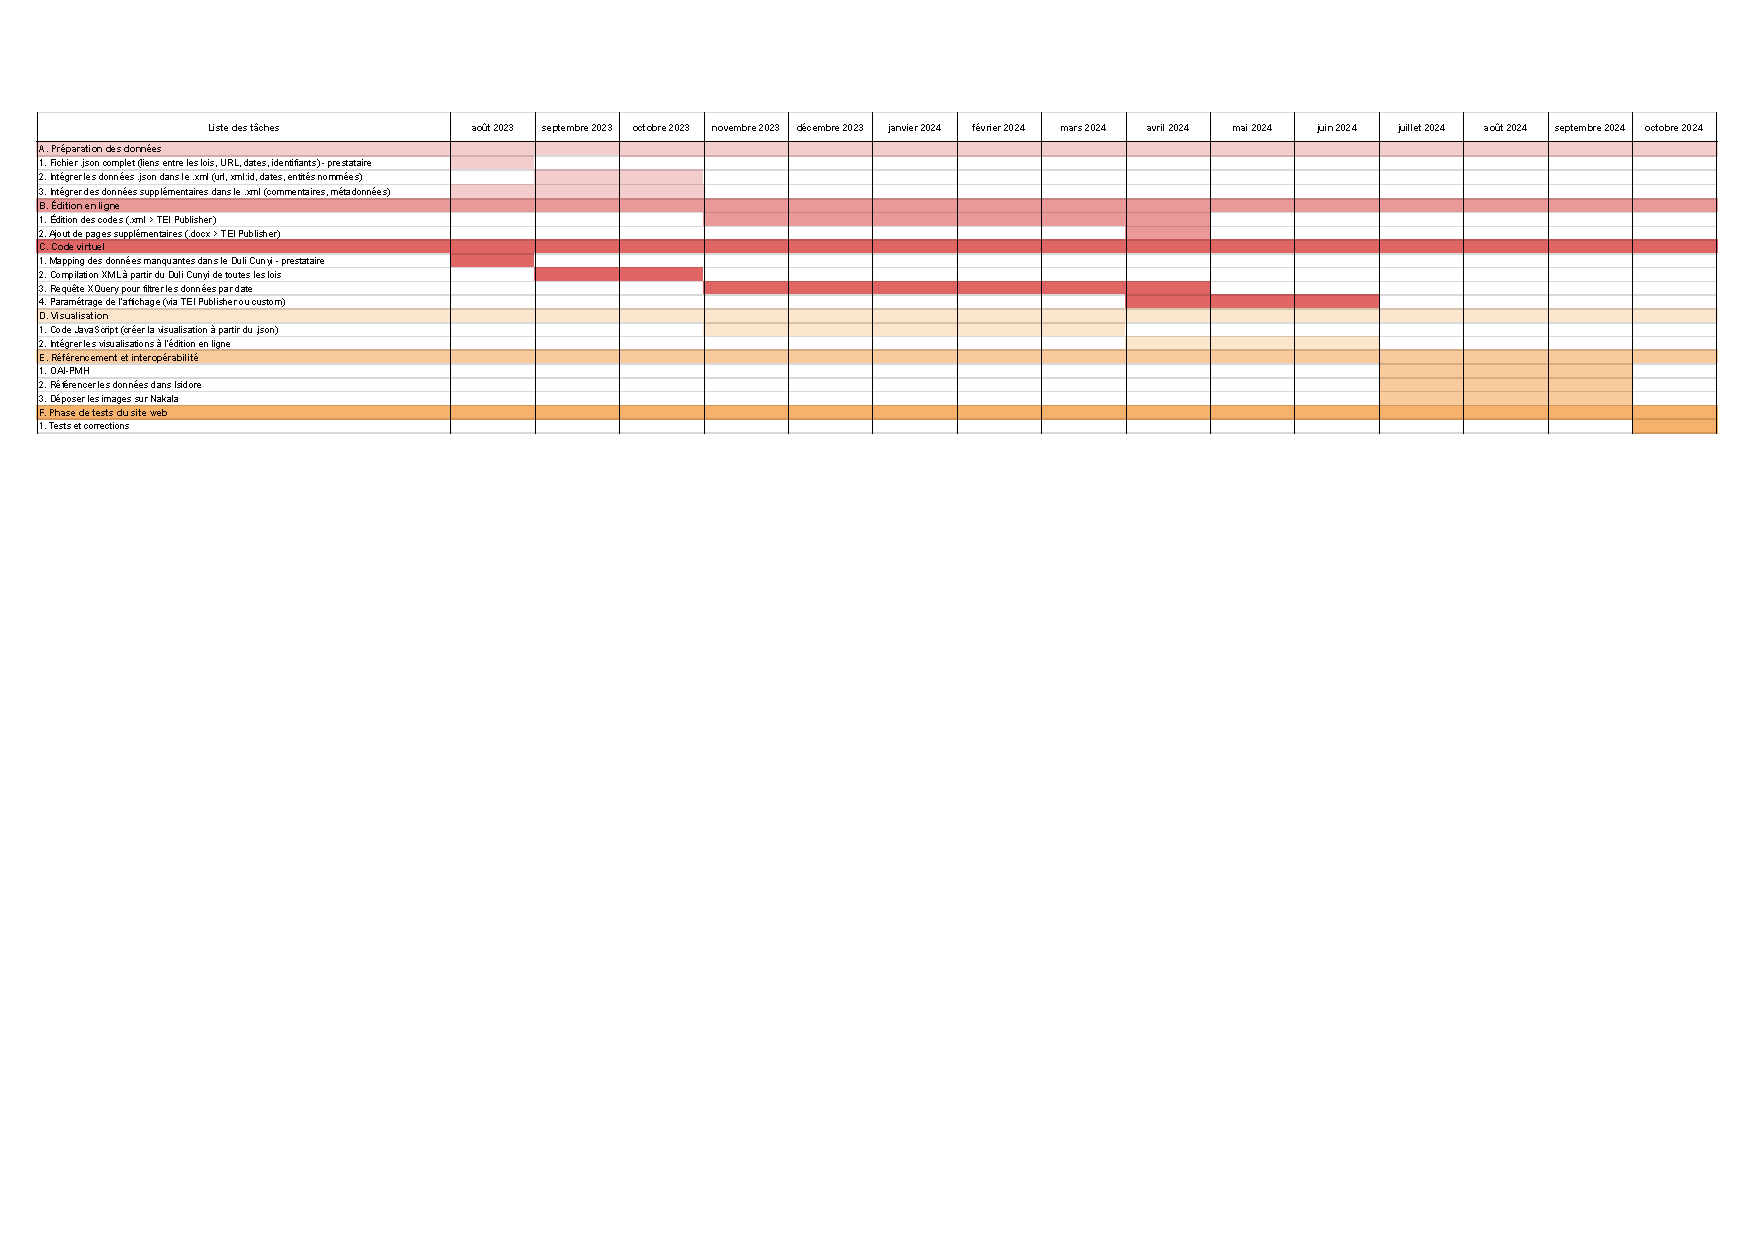
\includepdf[page={1},angle=90]{annexes/calendrier.pdf}
    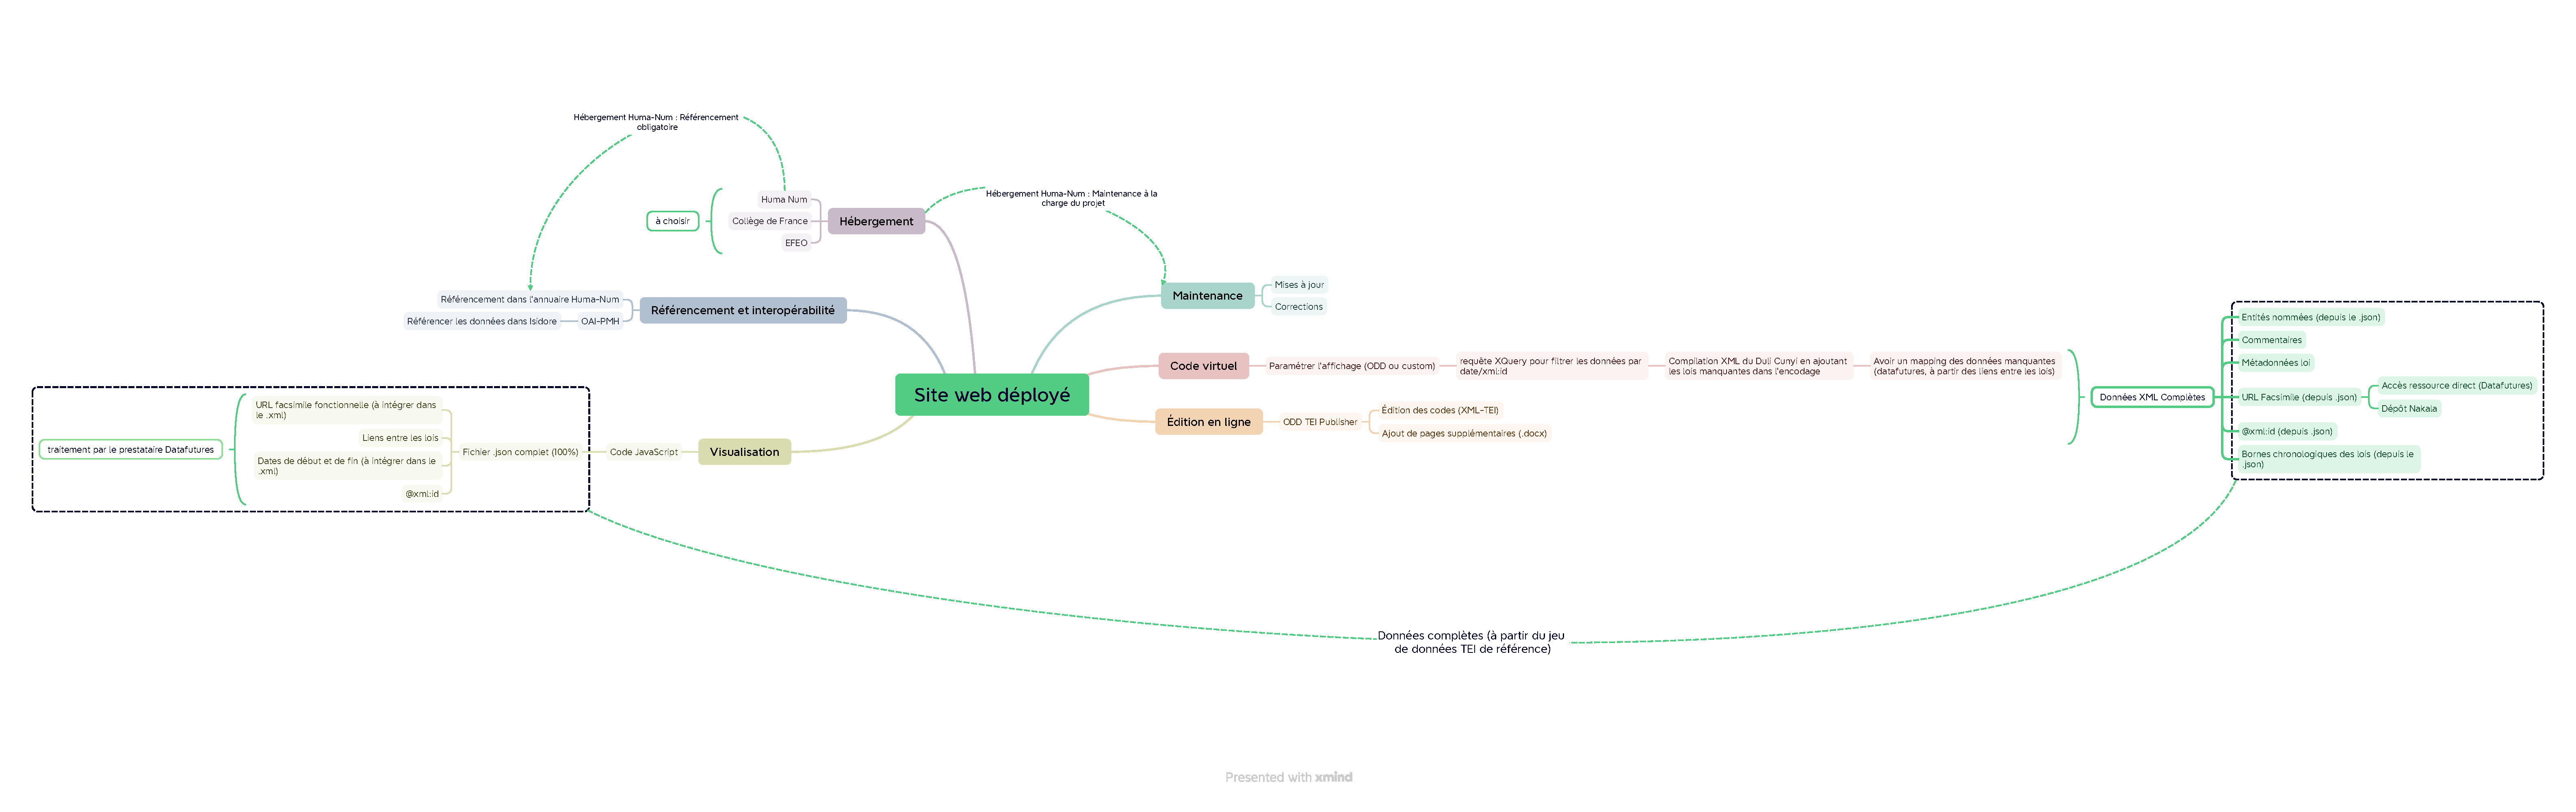
\includepdf[page={1}, angle=90]{annexes/mindmap.pdf}
\end{landscape}

\newpage
\section*{Maquettes}
\noindent 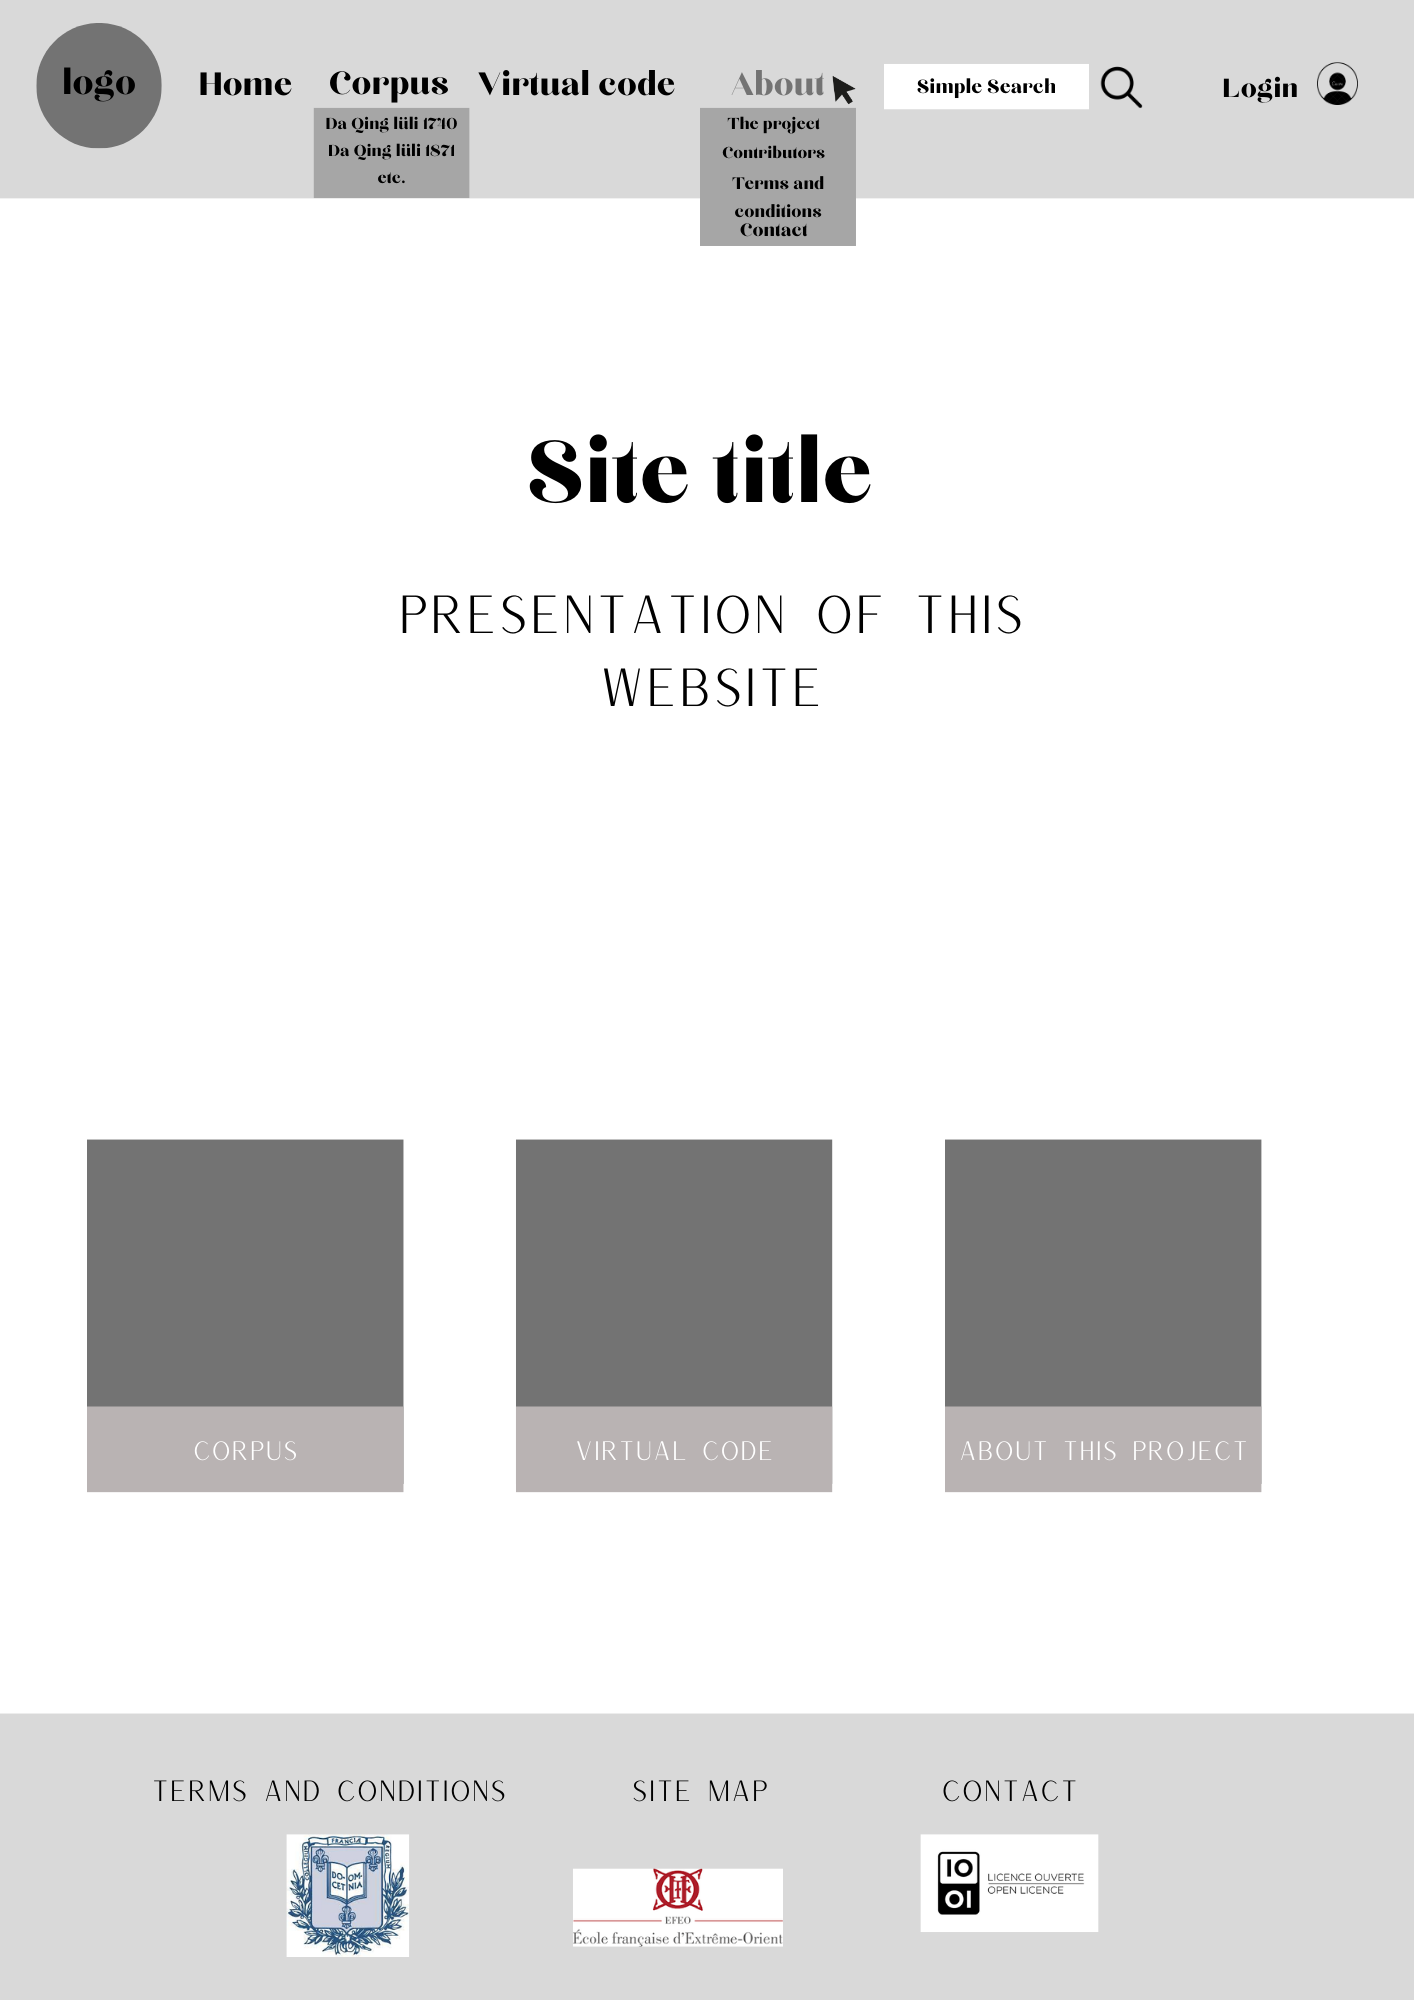
\includegraphics[width=\textwidth]{annexes/1 - Accueil.png}
\noindent 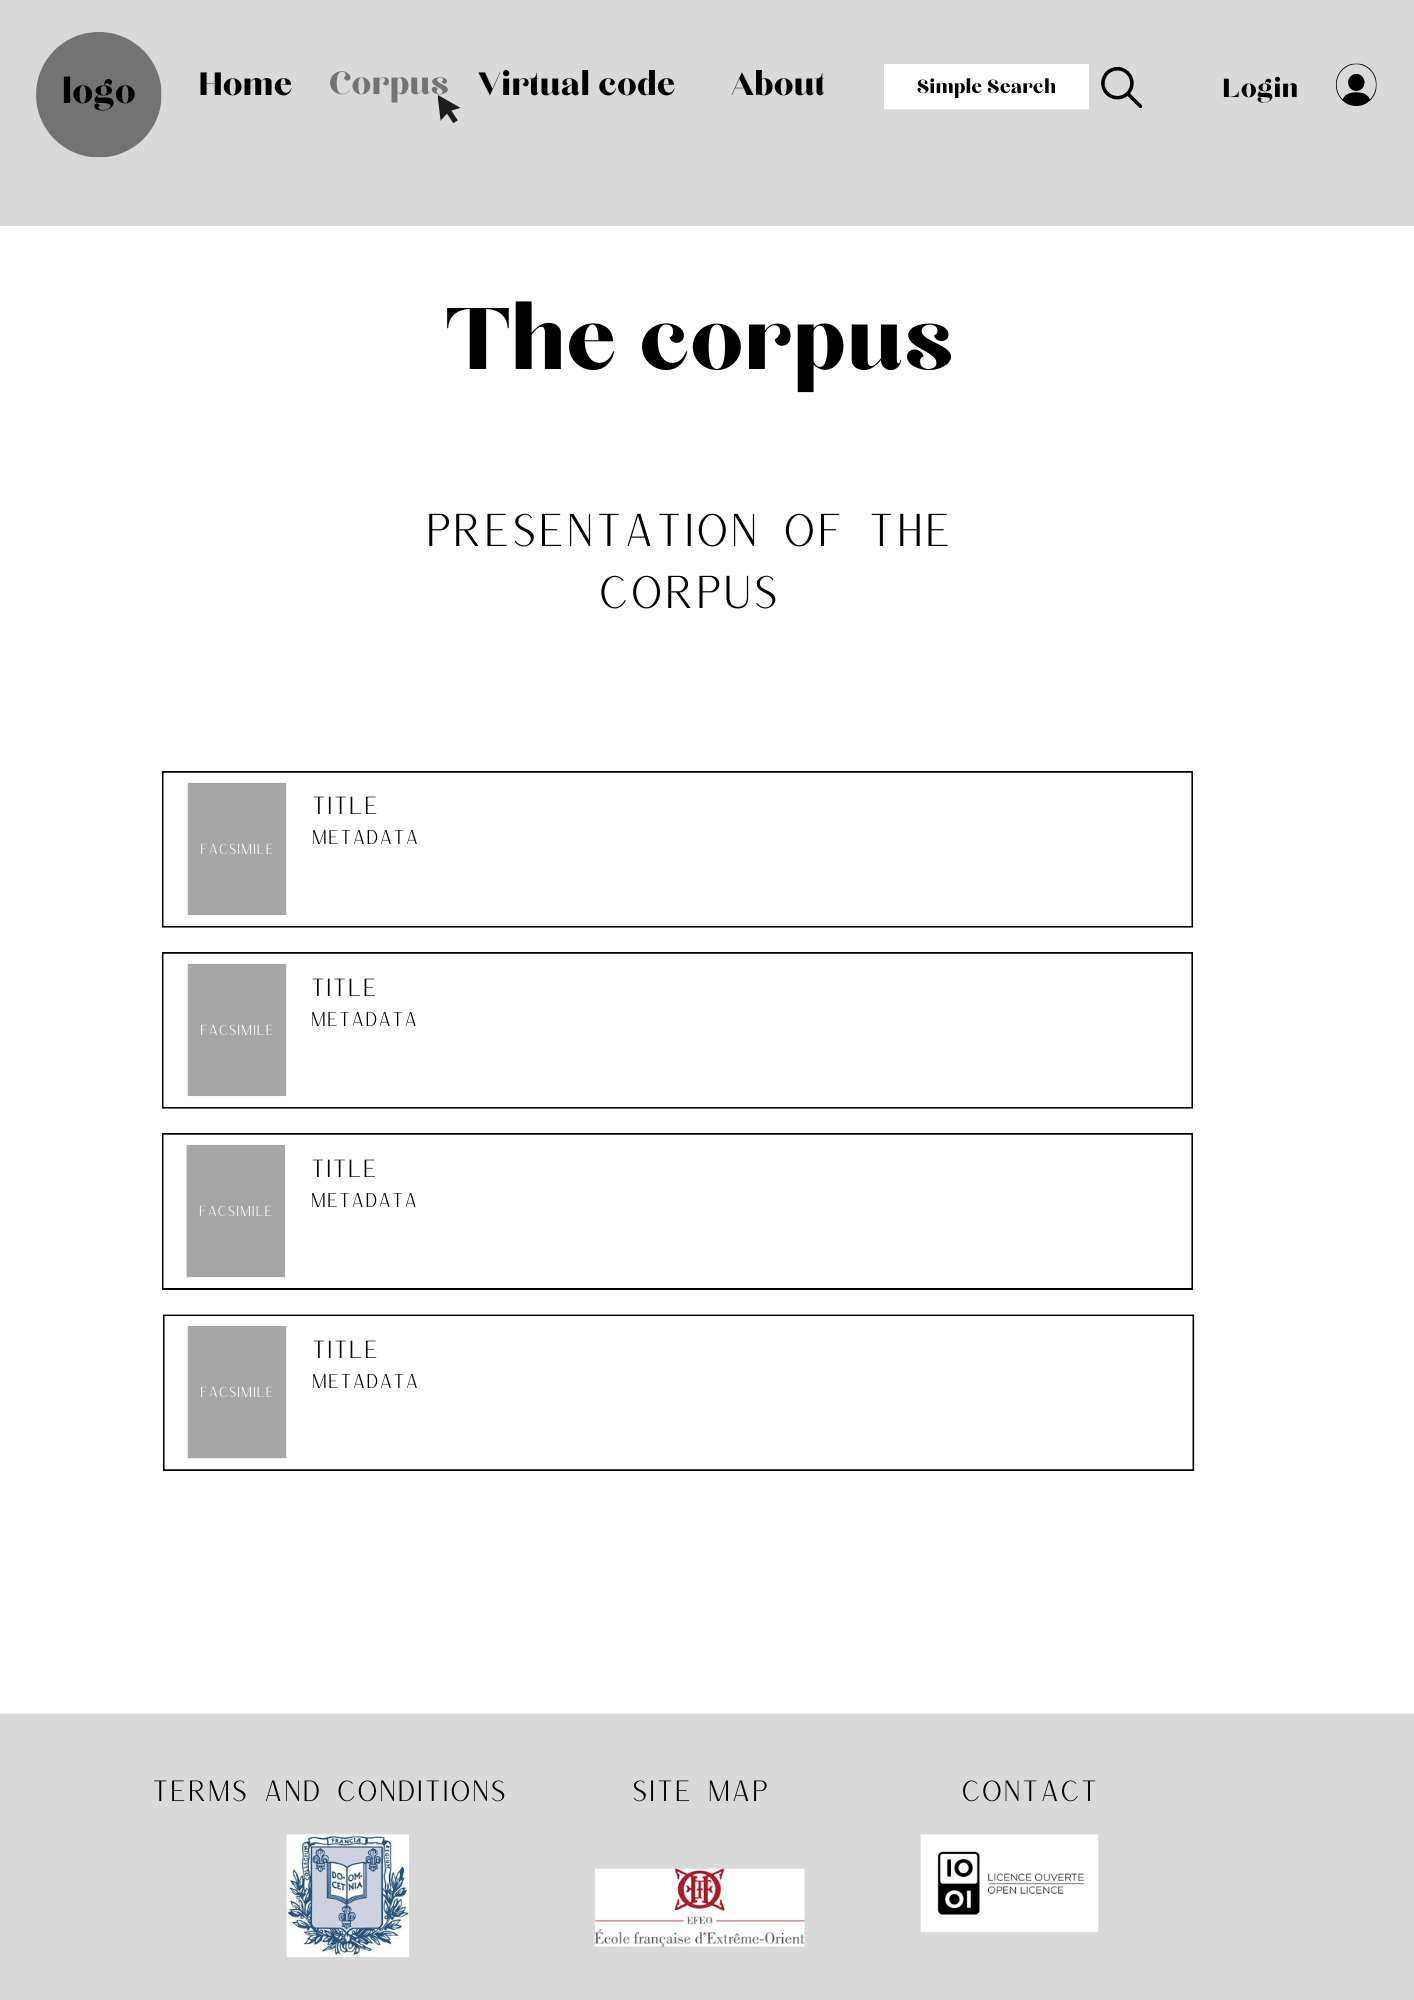
\includegraphics[width=\textwidth]{annexes/2-Corpus.png}
\noindent \includegraphics[width=\textwidth]{annexes/3 - Édition en ligne _ commentaires.png}
\noindent 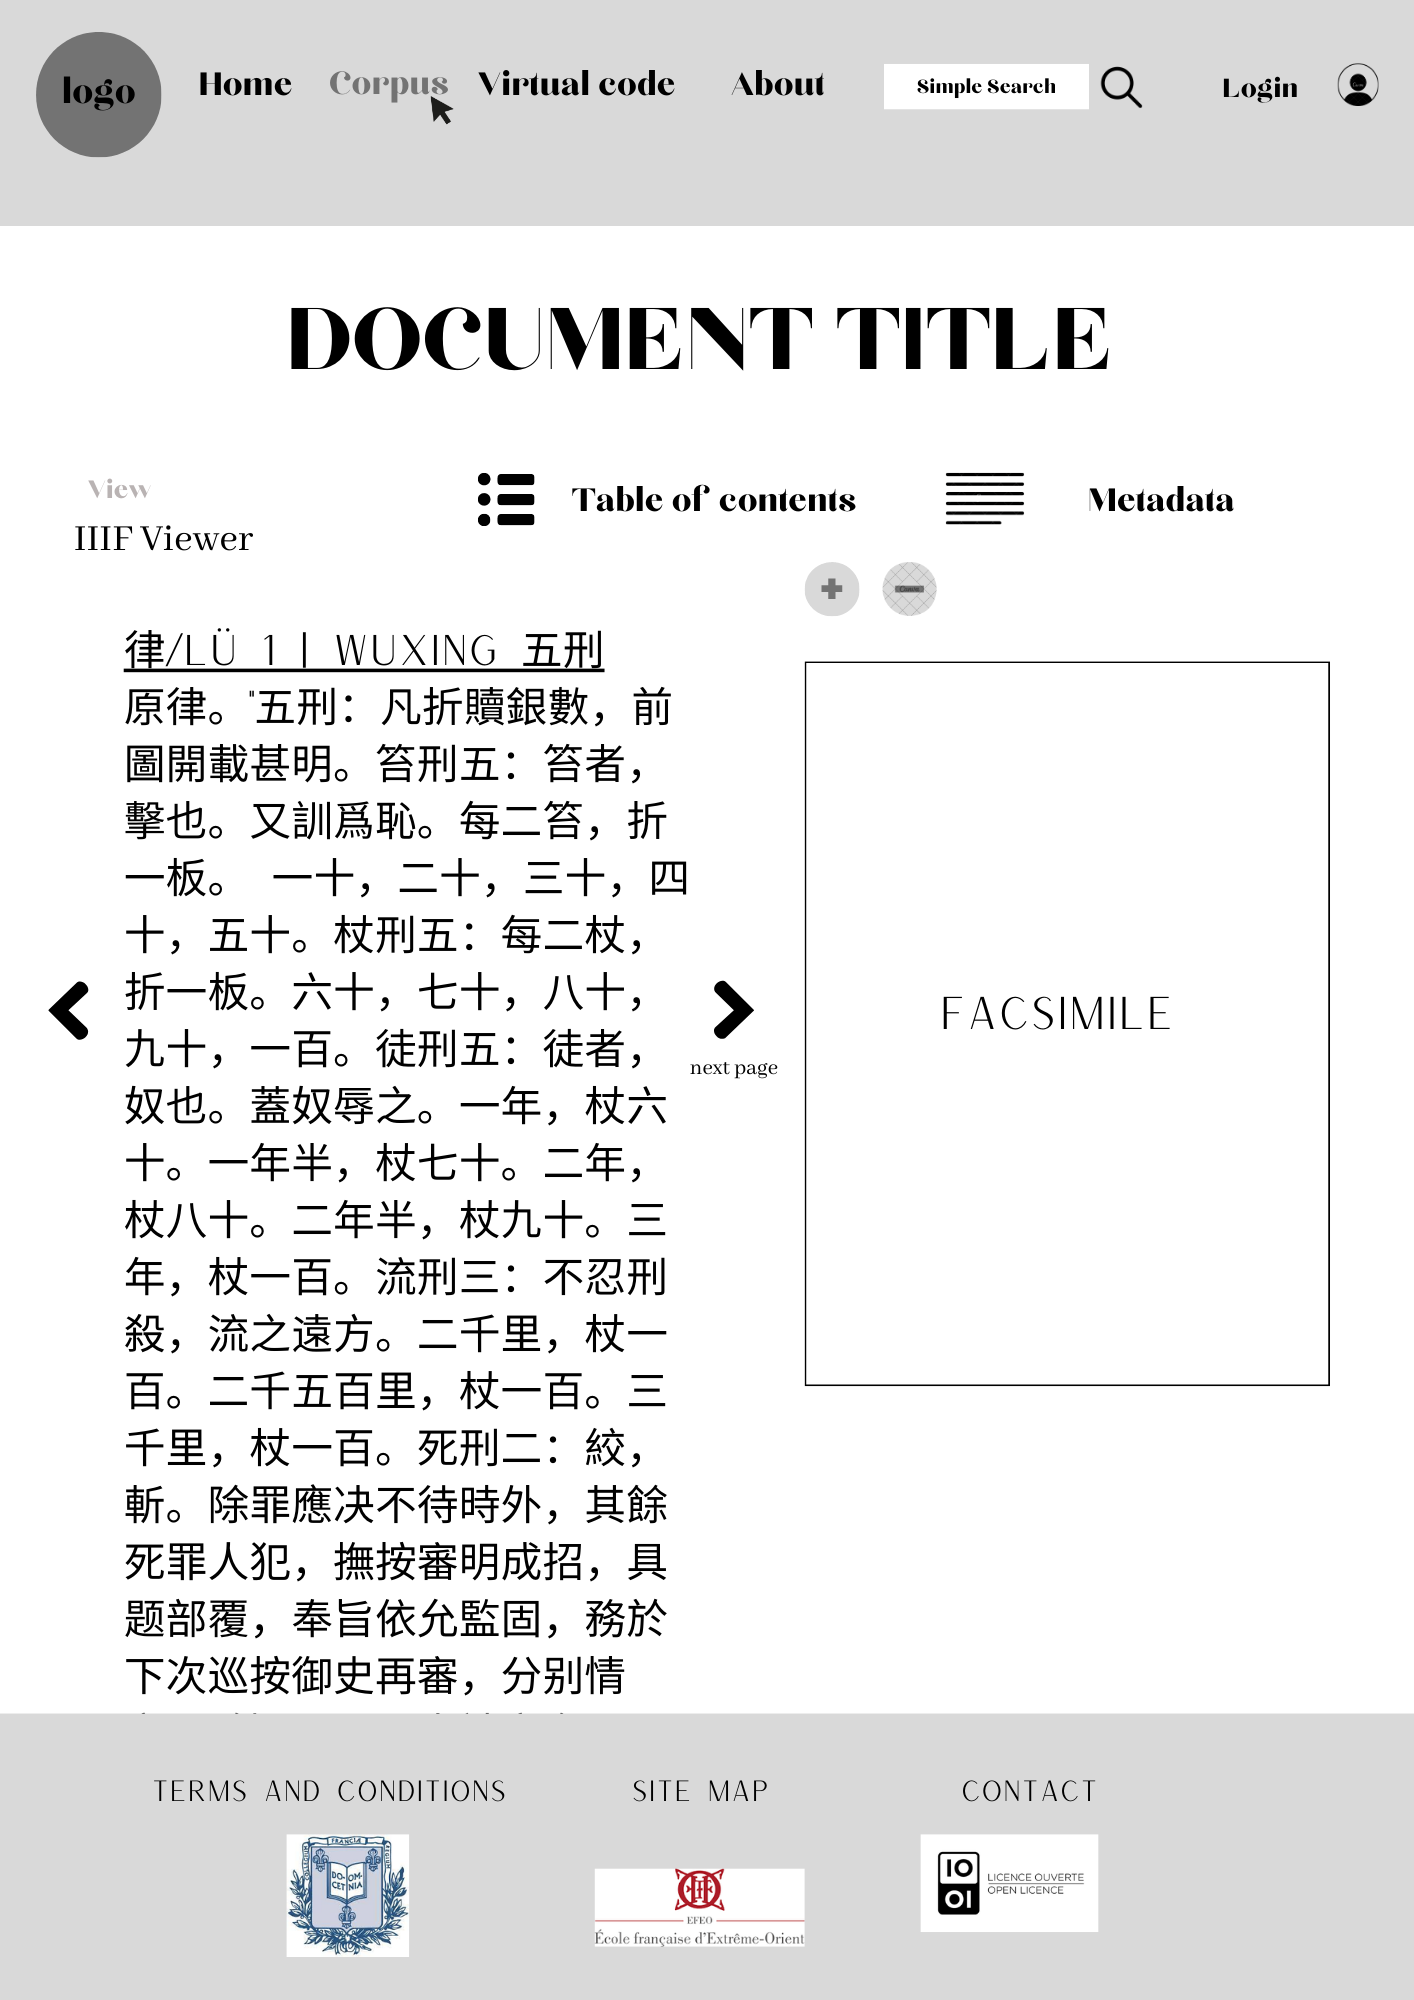
\includegraphics[width=\textwidth]{annexes/4 - Édition en ligne _ fac similé.png}
\noindent 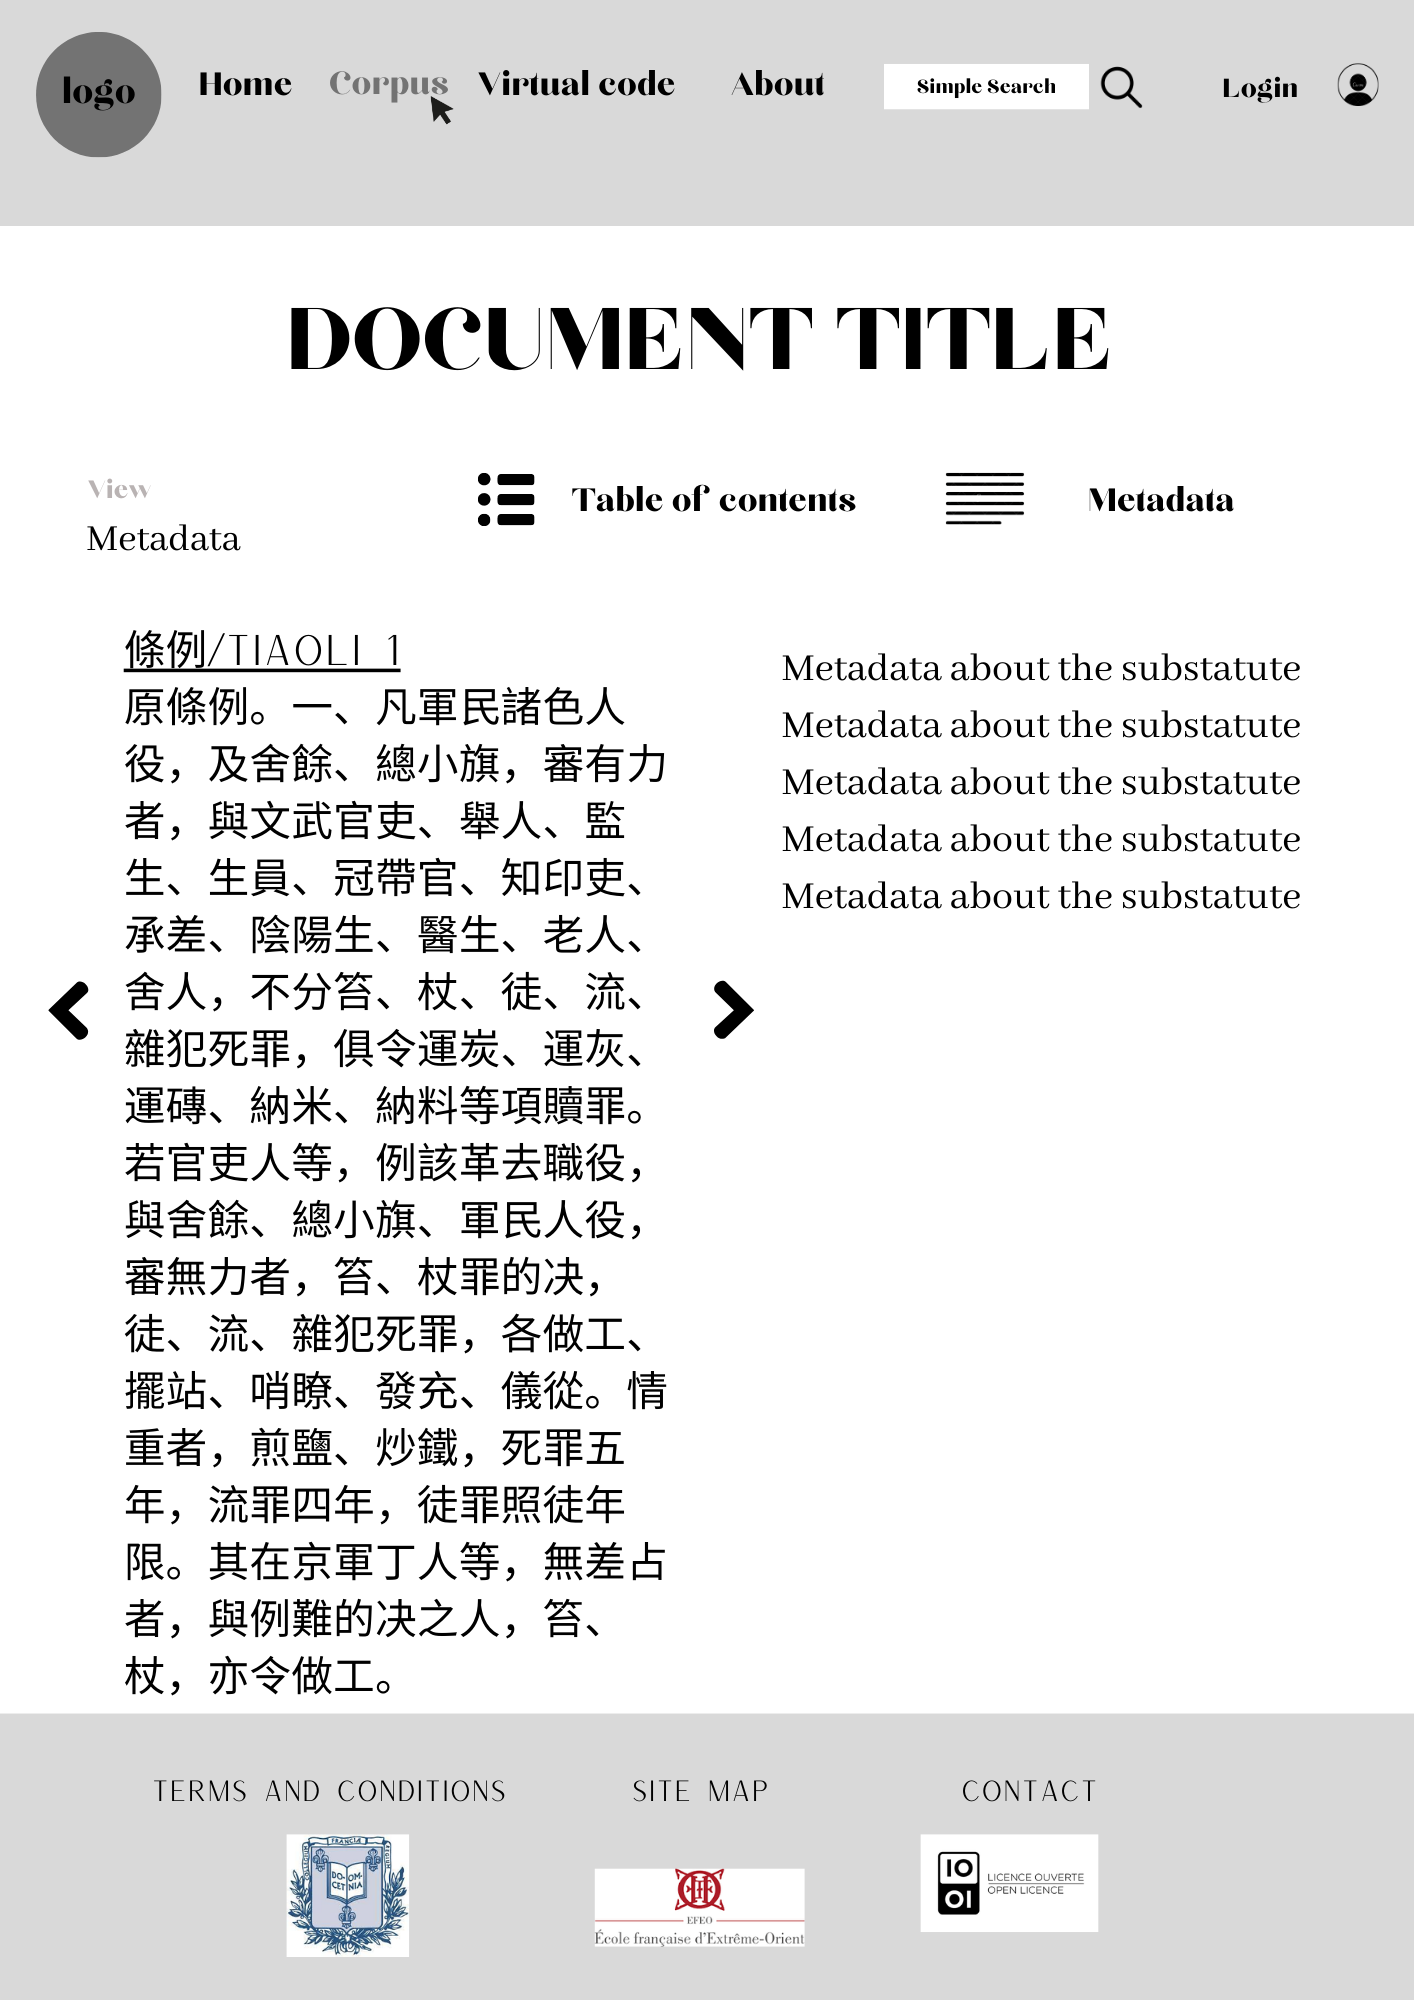
\includegraphics[width=\textwidth]{annexes/5 - Édition en ligne _ métadonnées.png}
\noindent 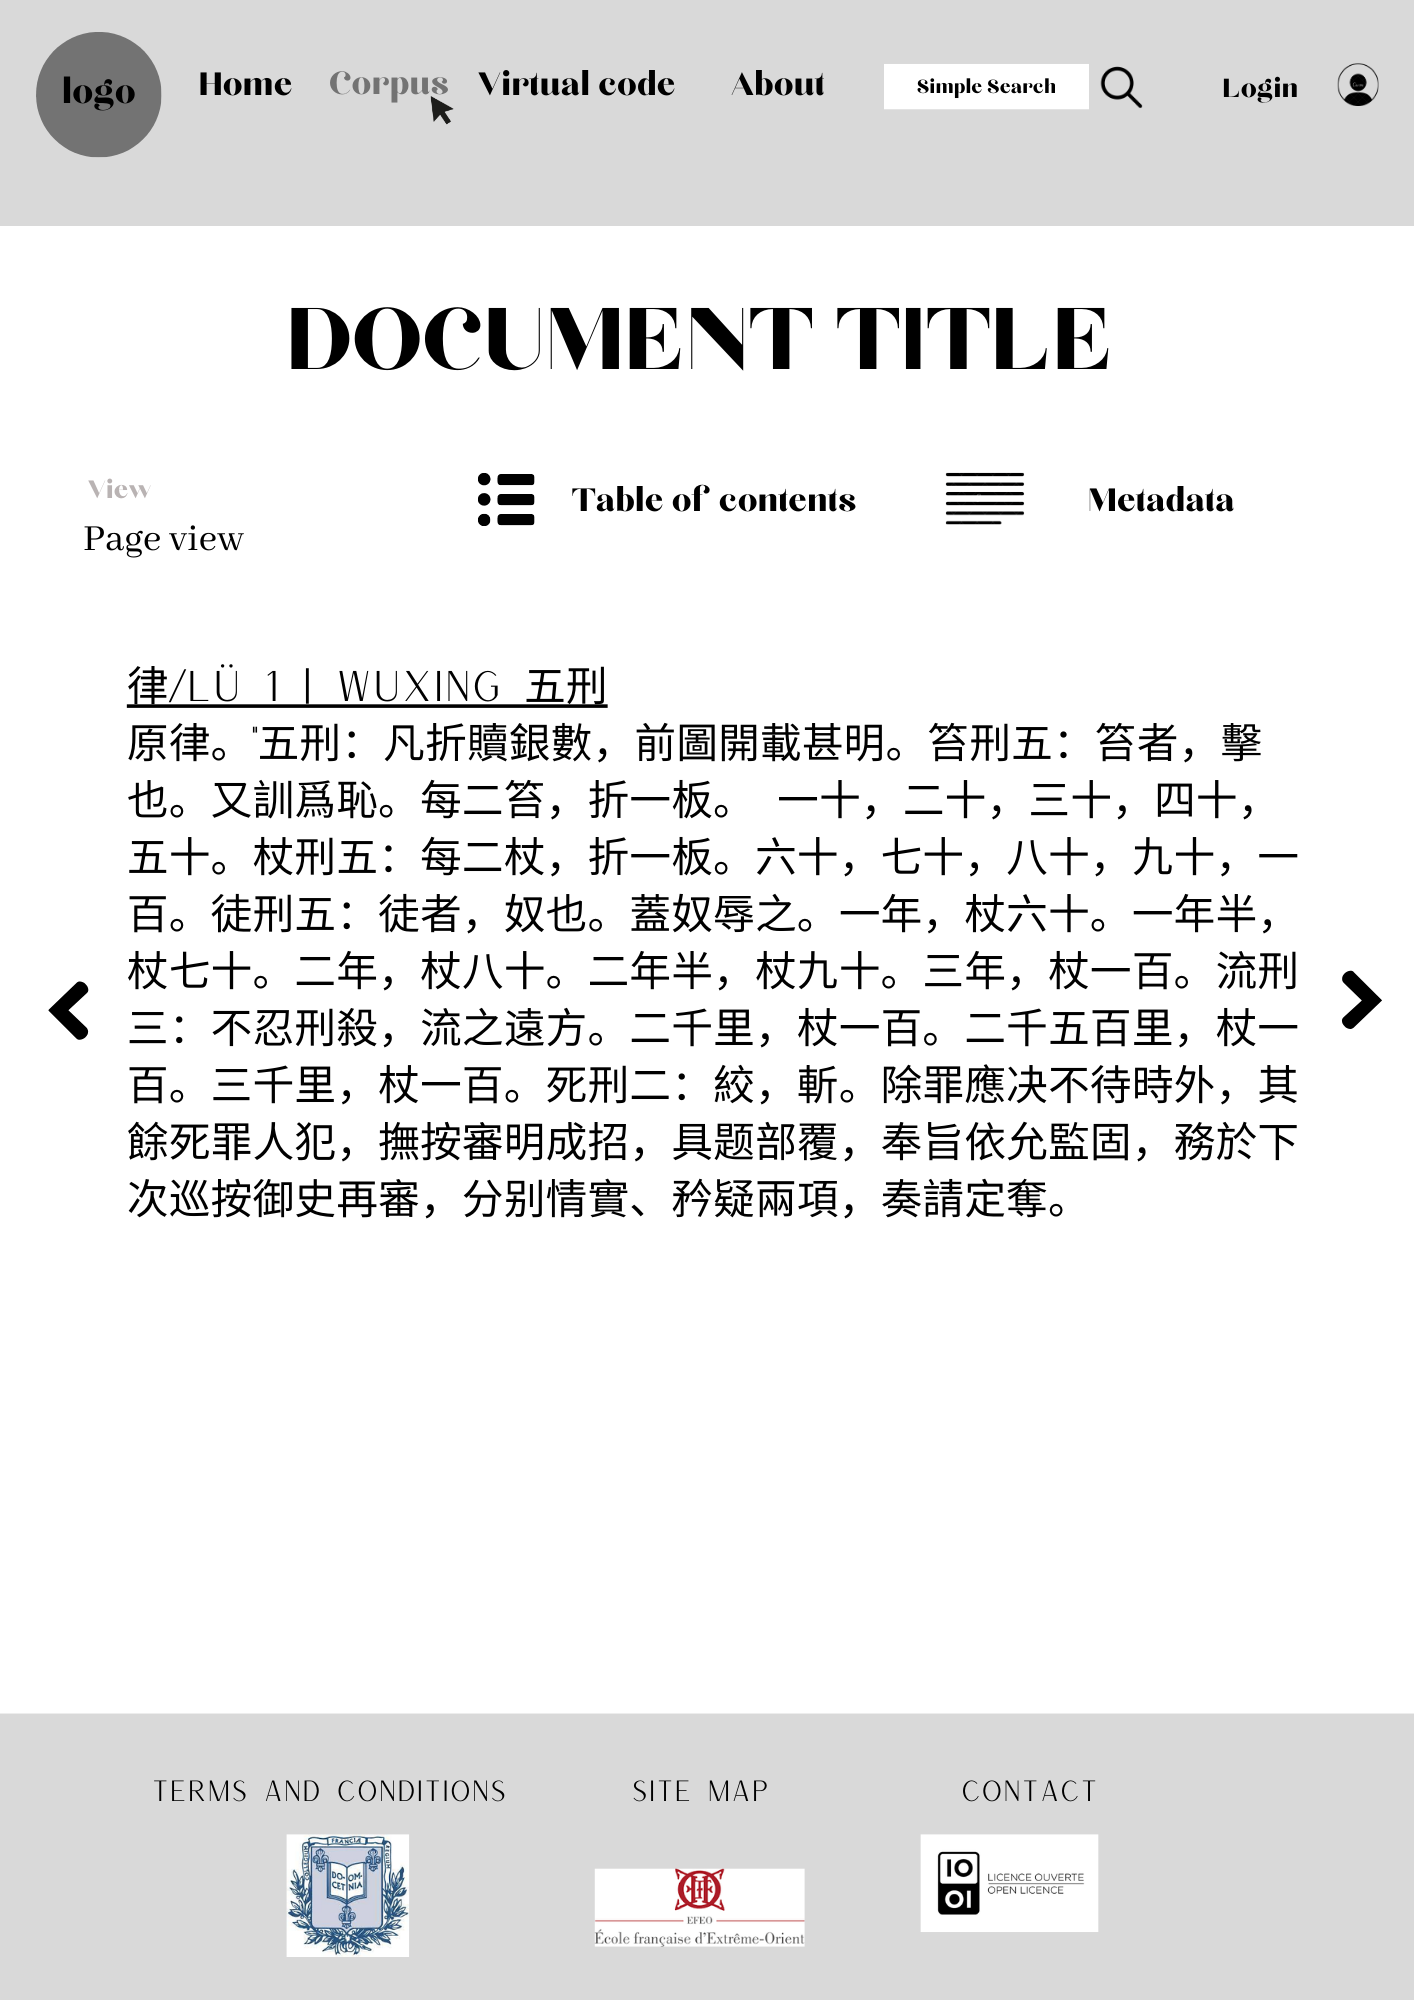
\includegraphics[width=\textwidth]{annexes/6 - Édition en ligne _ texte paginé.png}
\noindent 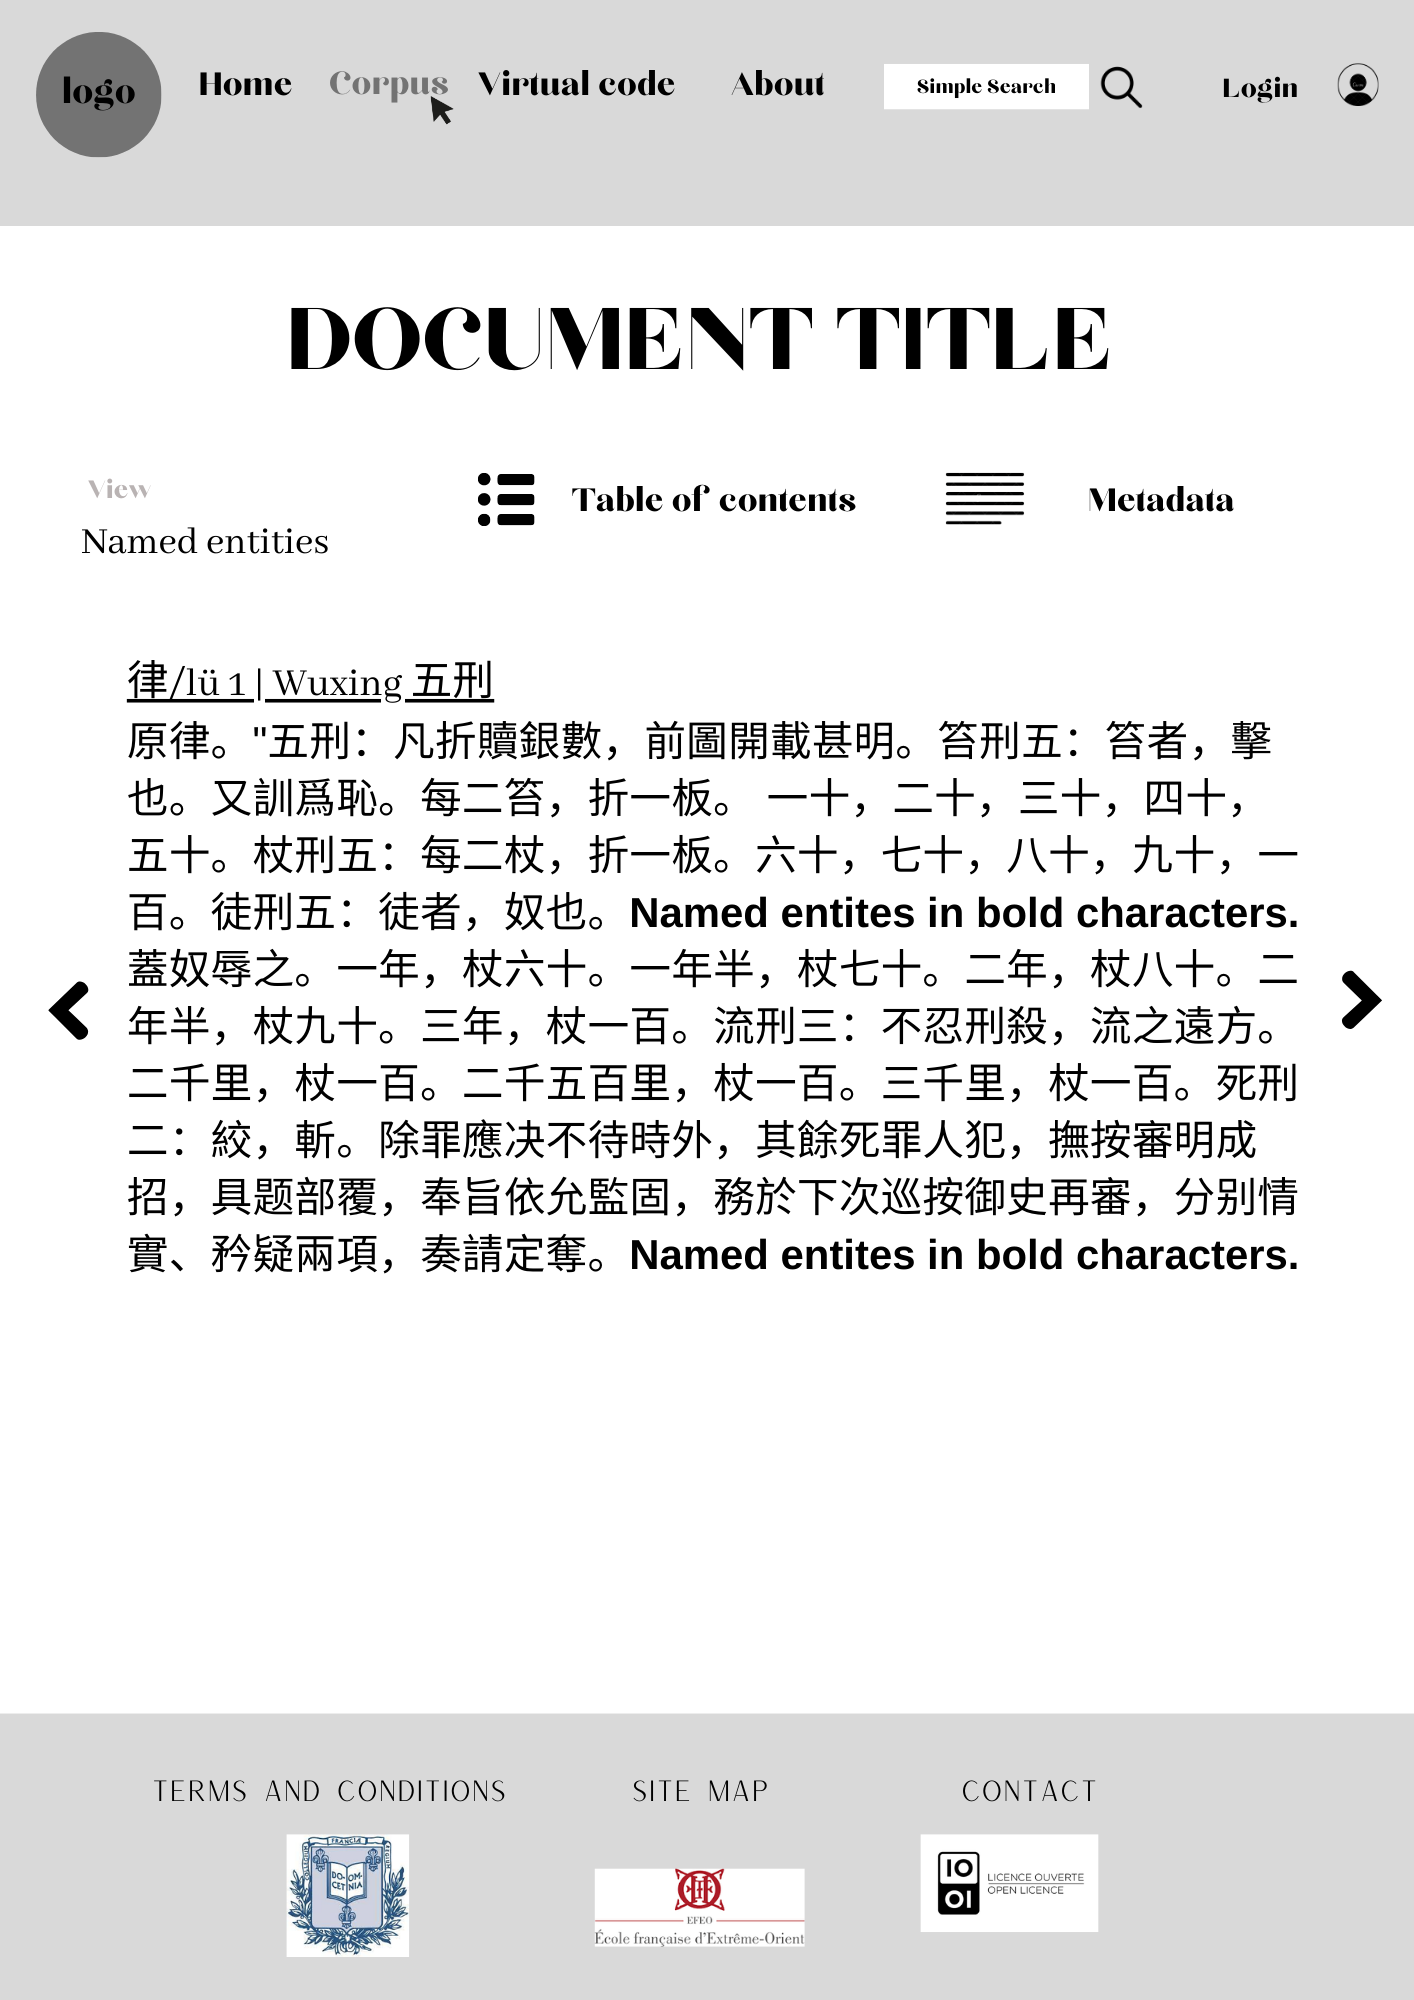
\includegraphics[width=\textwidth]{annexes/7 - Mode _ entités nommées.png}
\noindent 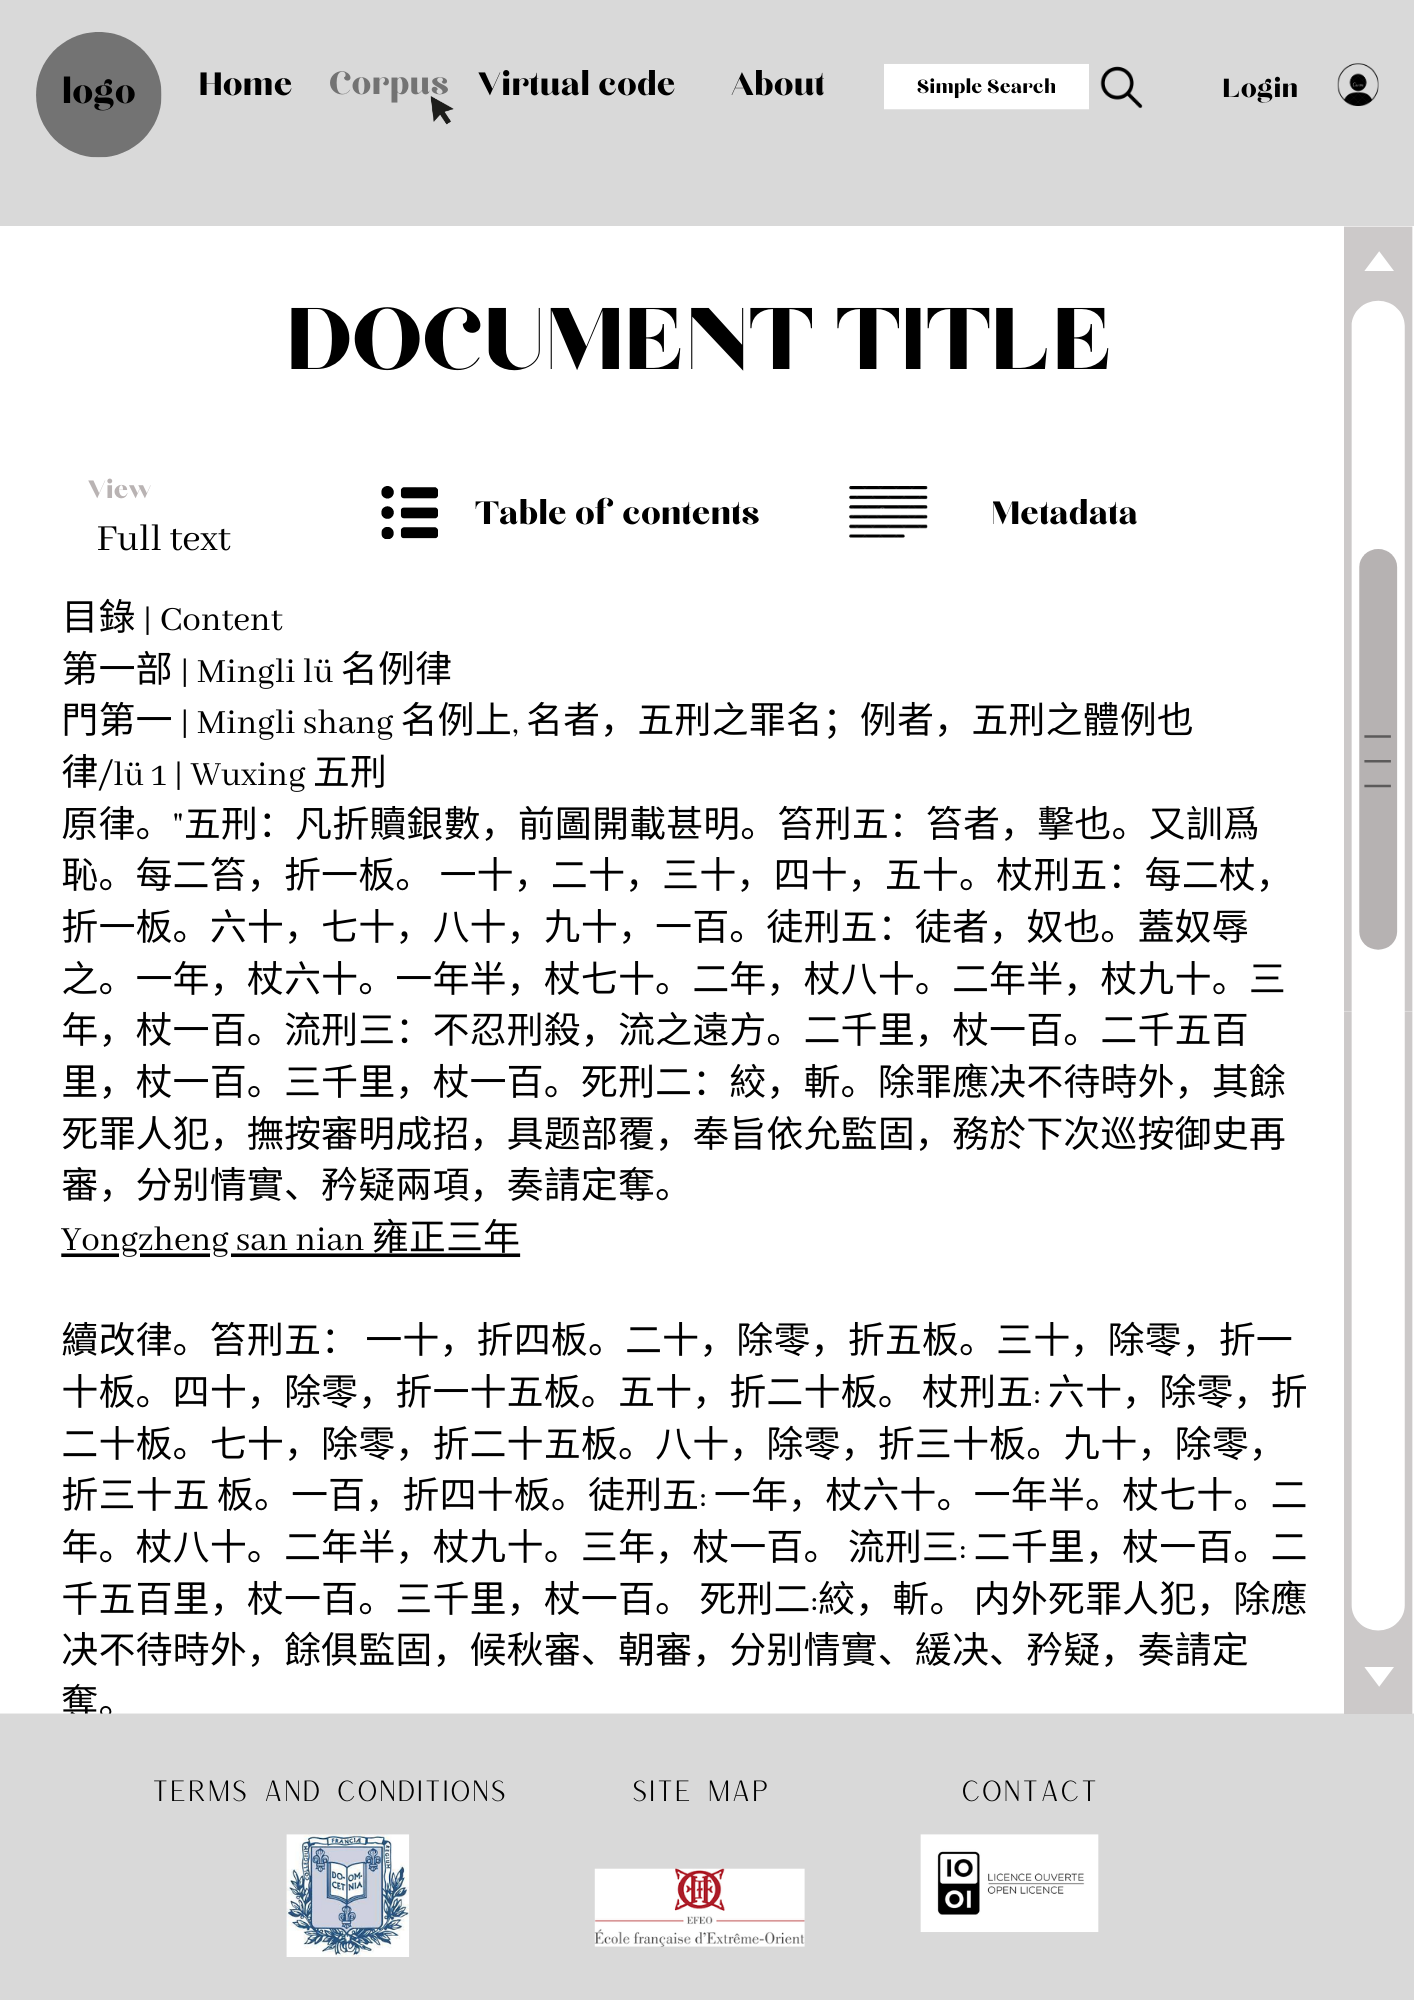
\includegraphics[width=\textwidth]{annexes/8 - Edition en ligne_Texte continu.png}
\noindent 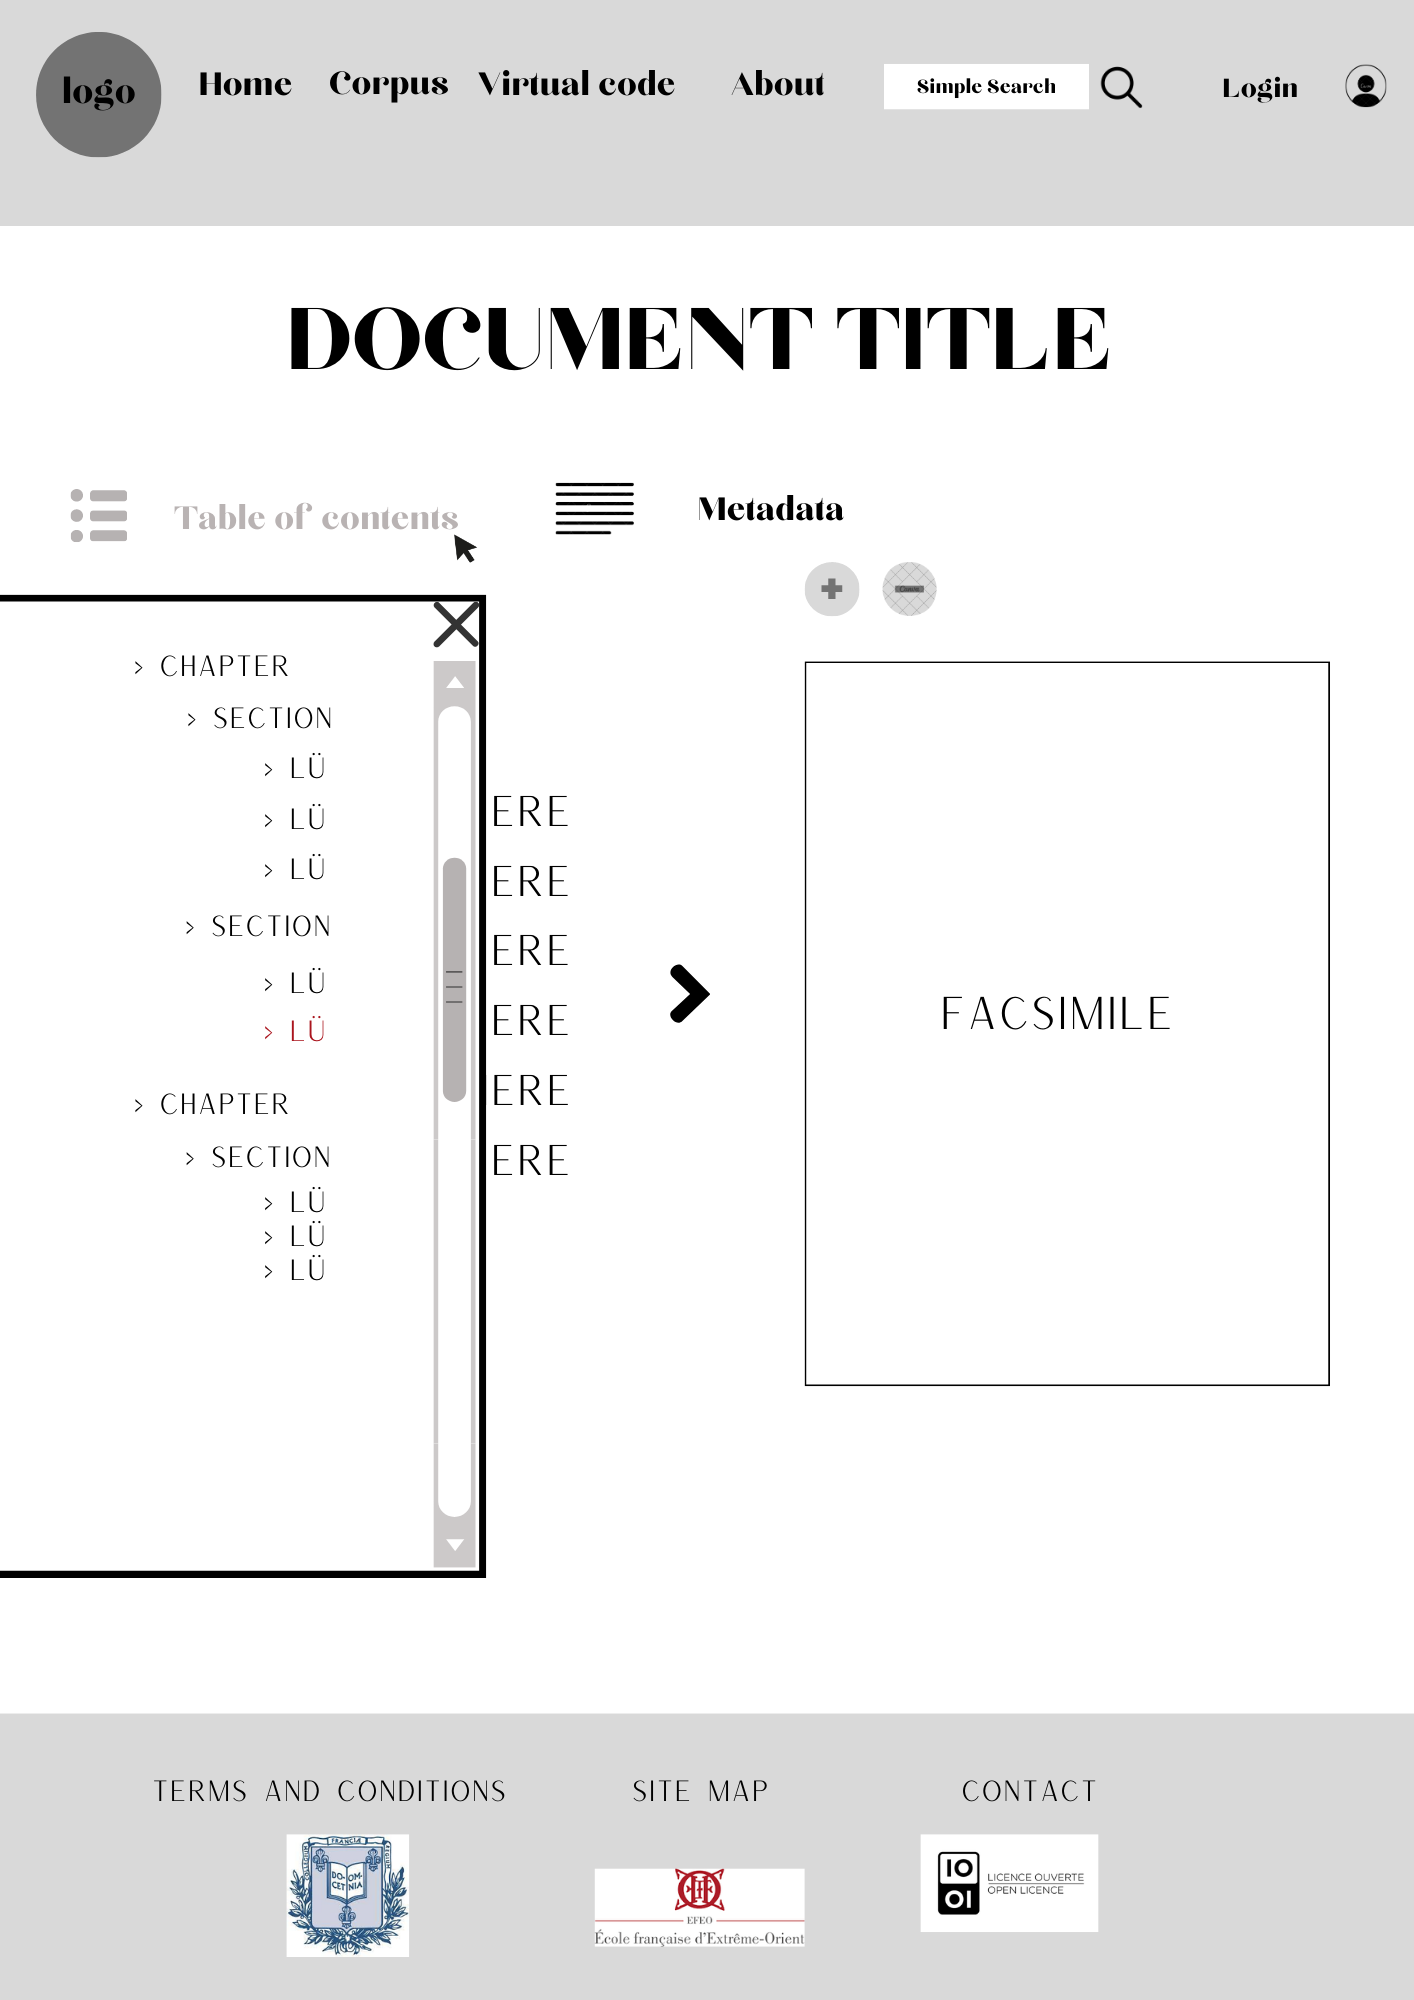
\includegraphics[width=\textwidth]{annexes/9 - Onglet toc.png}
\noindent 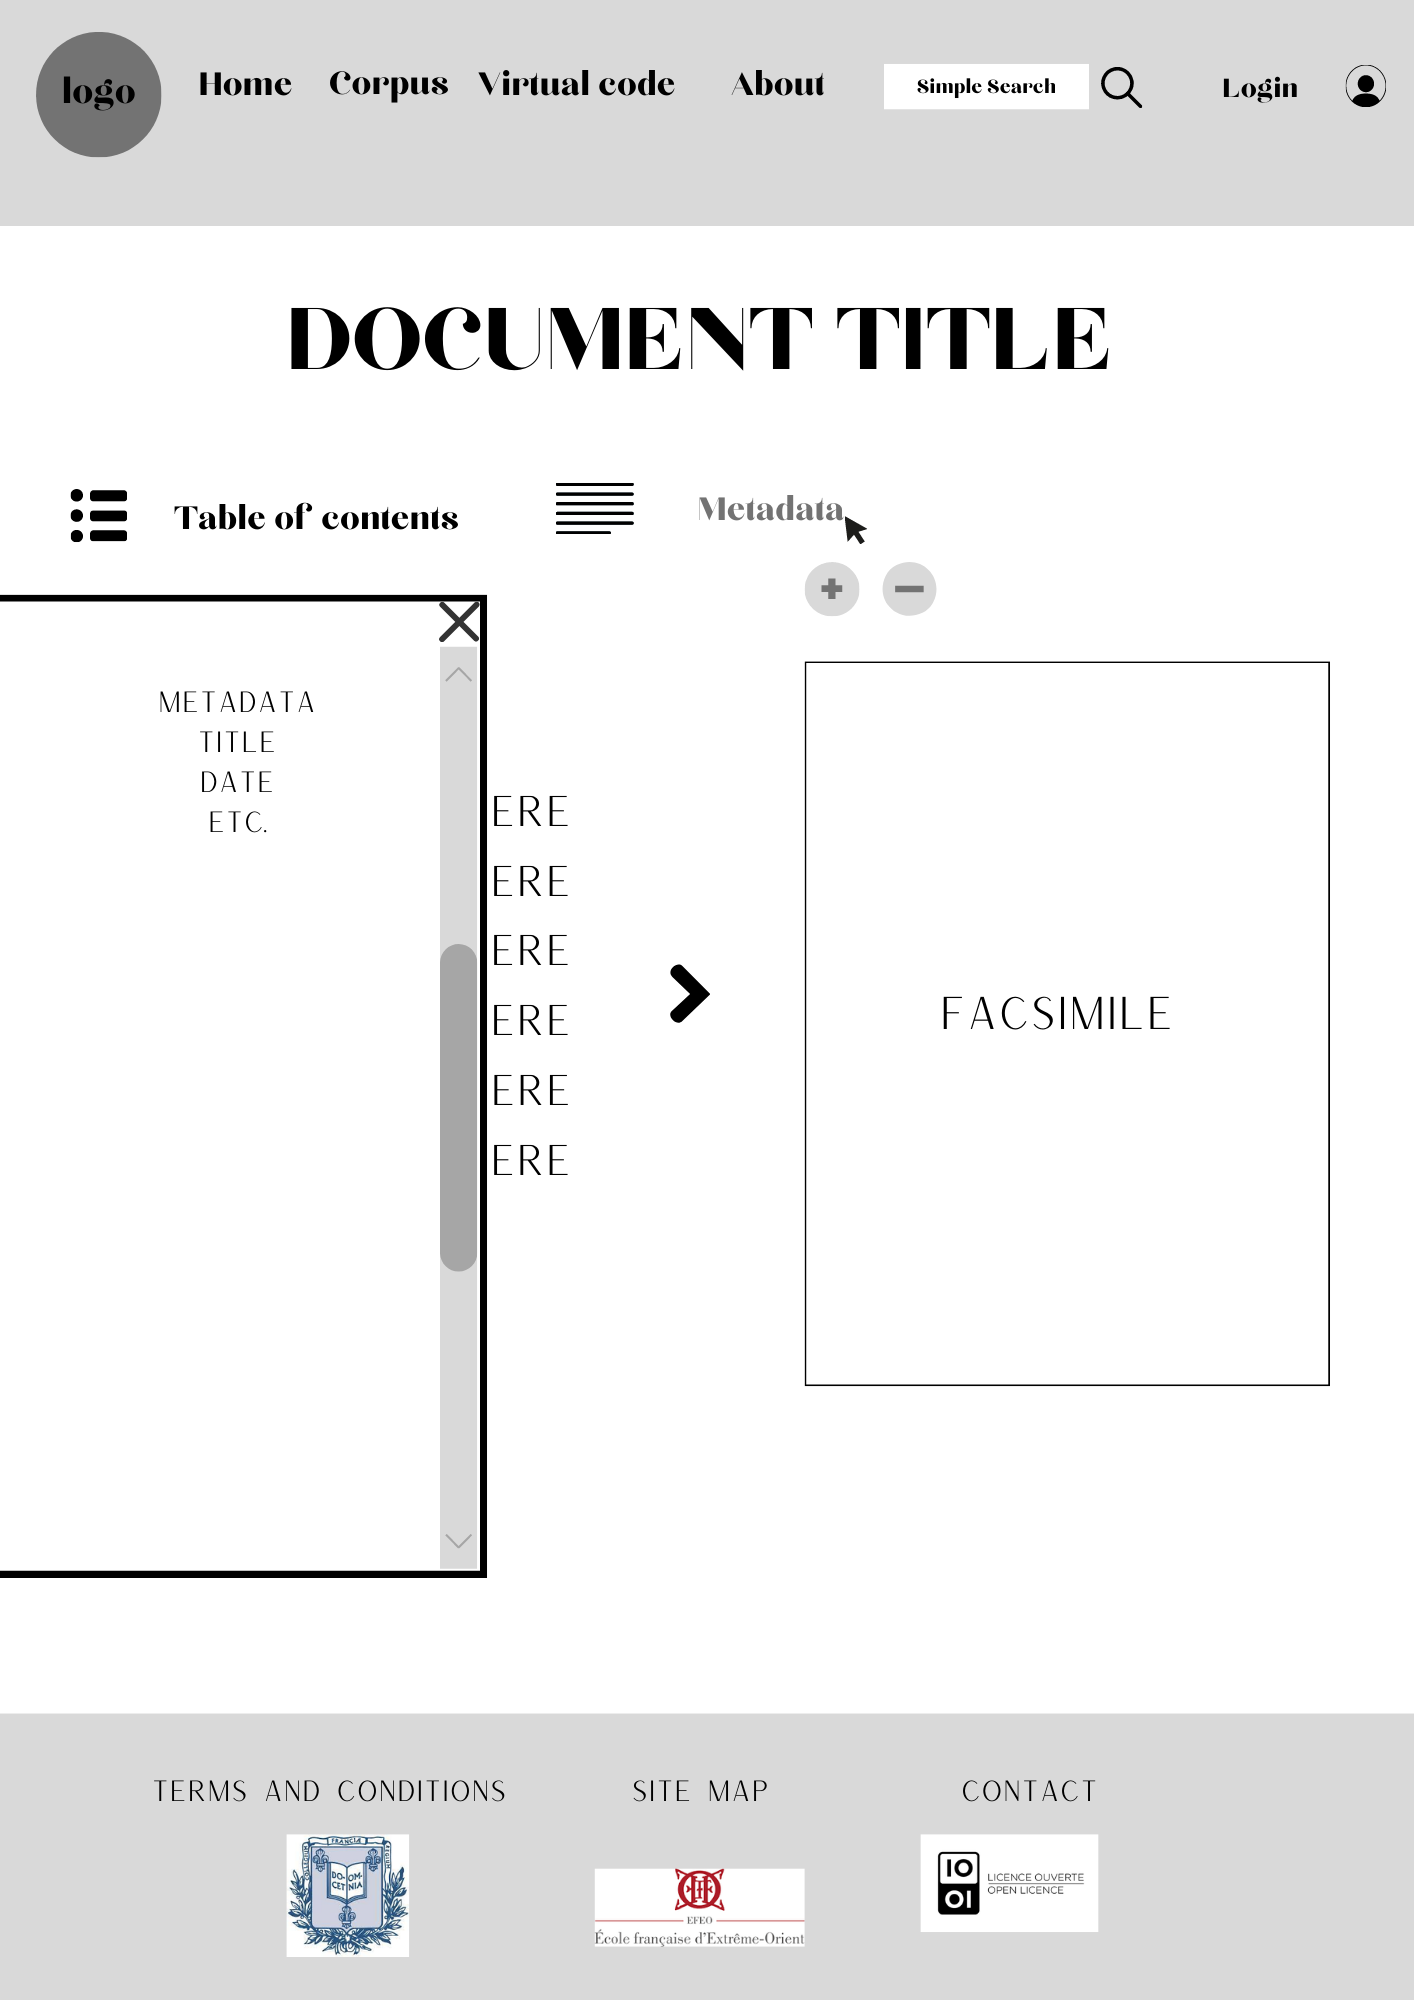
\includegraphics[width=\textwidth]{annexes/10 - Onglet métadonnées.png}
\noindent 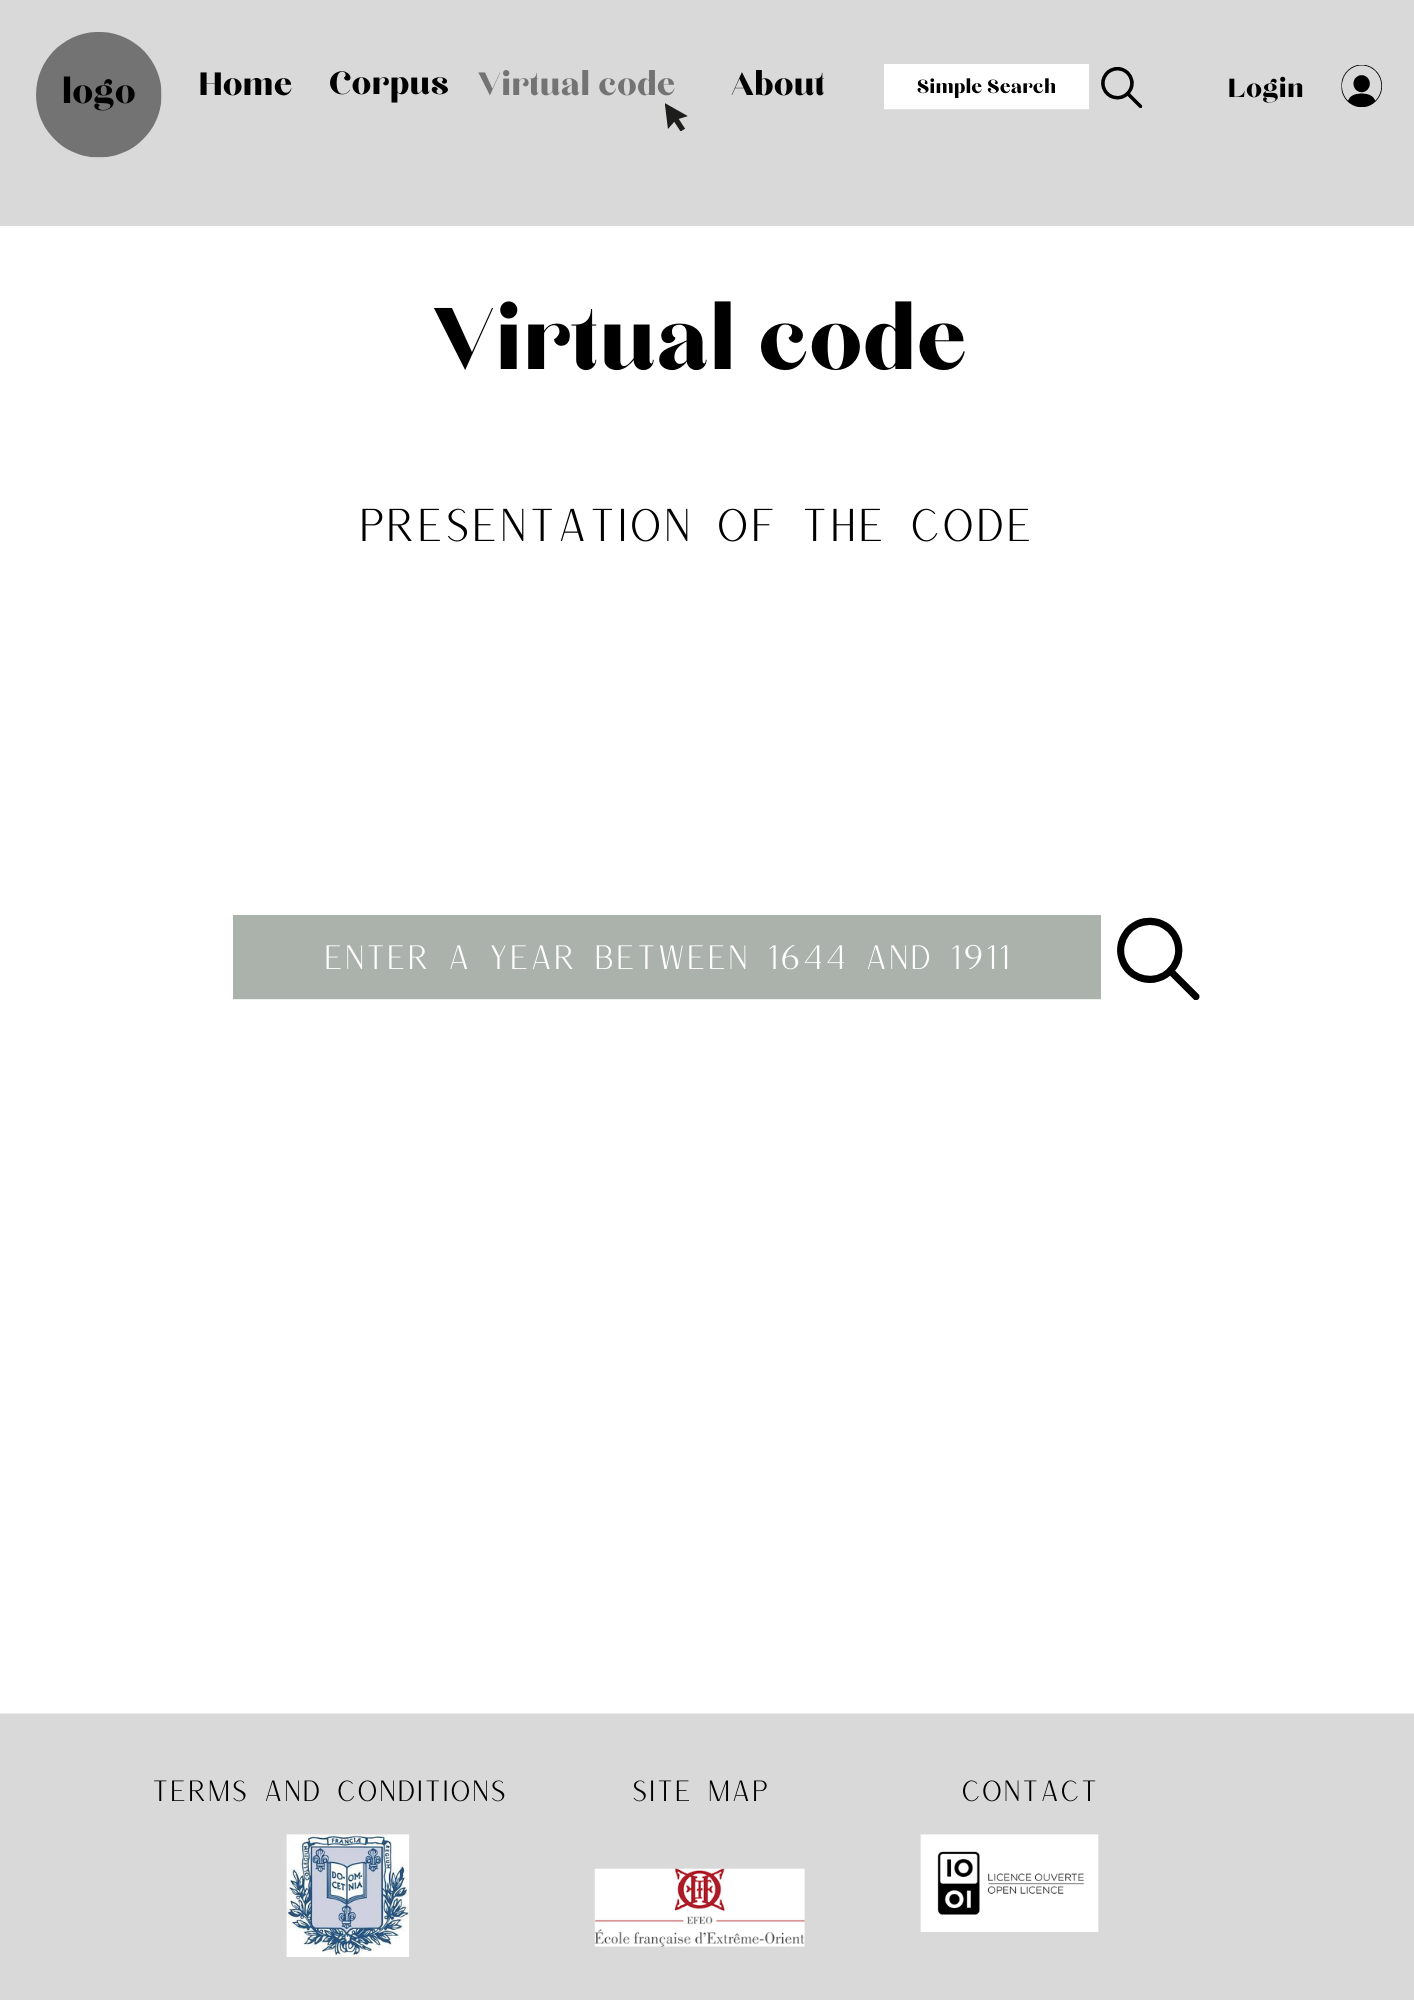
\includegraphics[width=\textwidth]{annexes/11 - Code virtuel (input).png}
\noindent 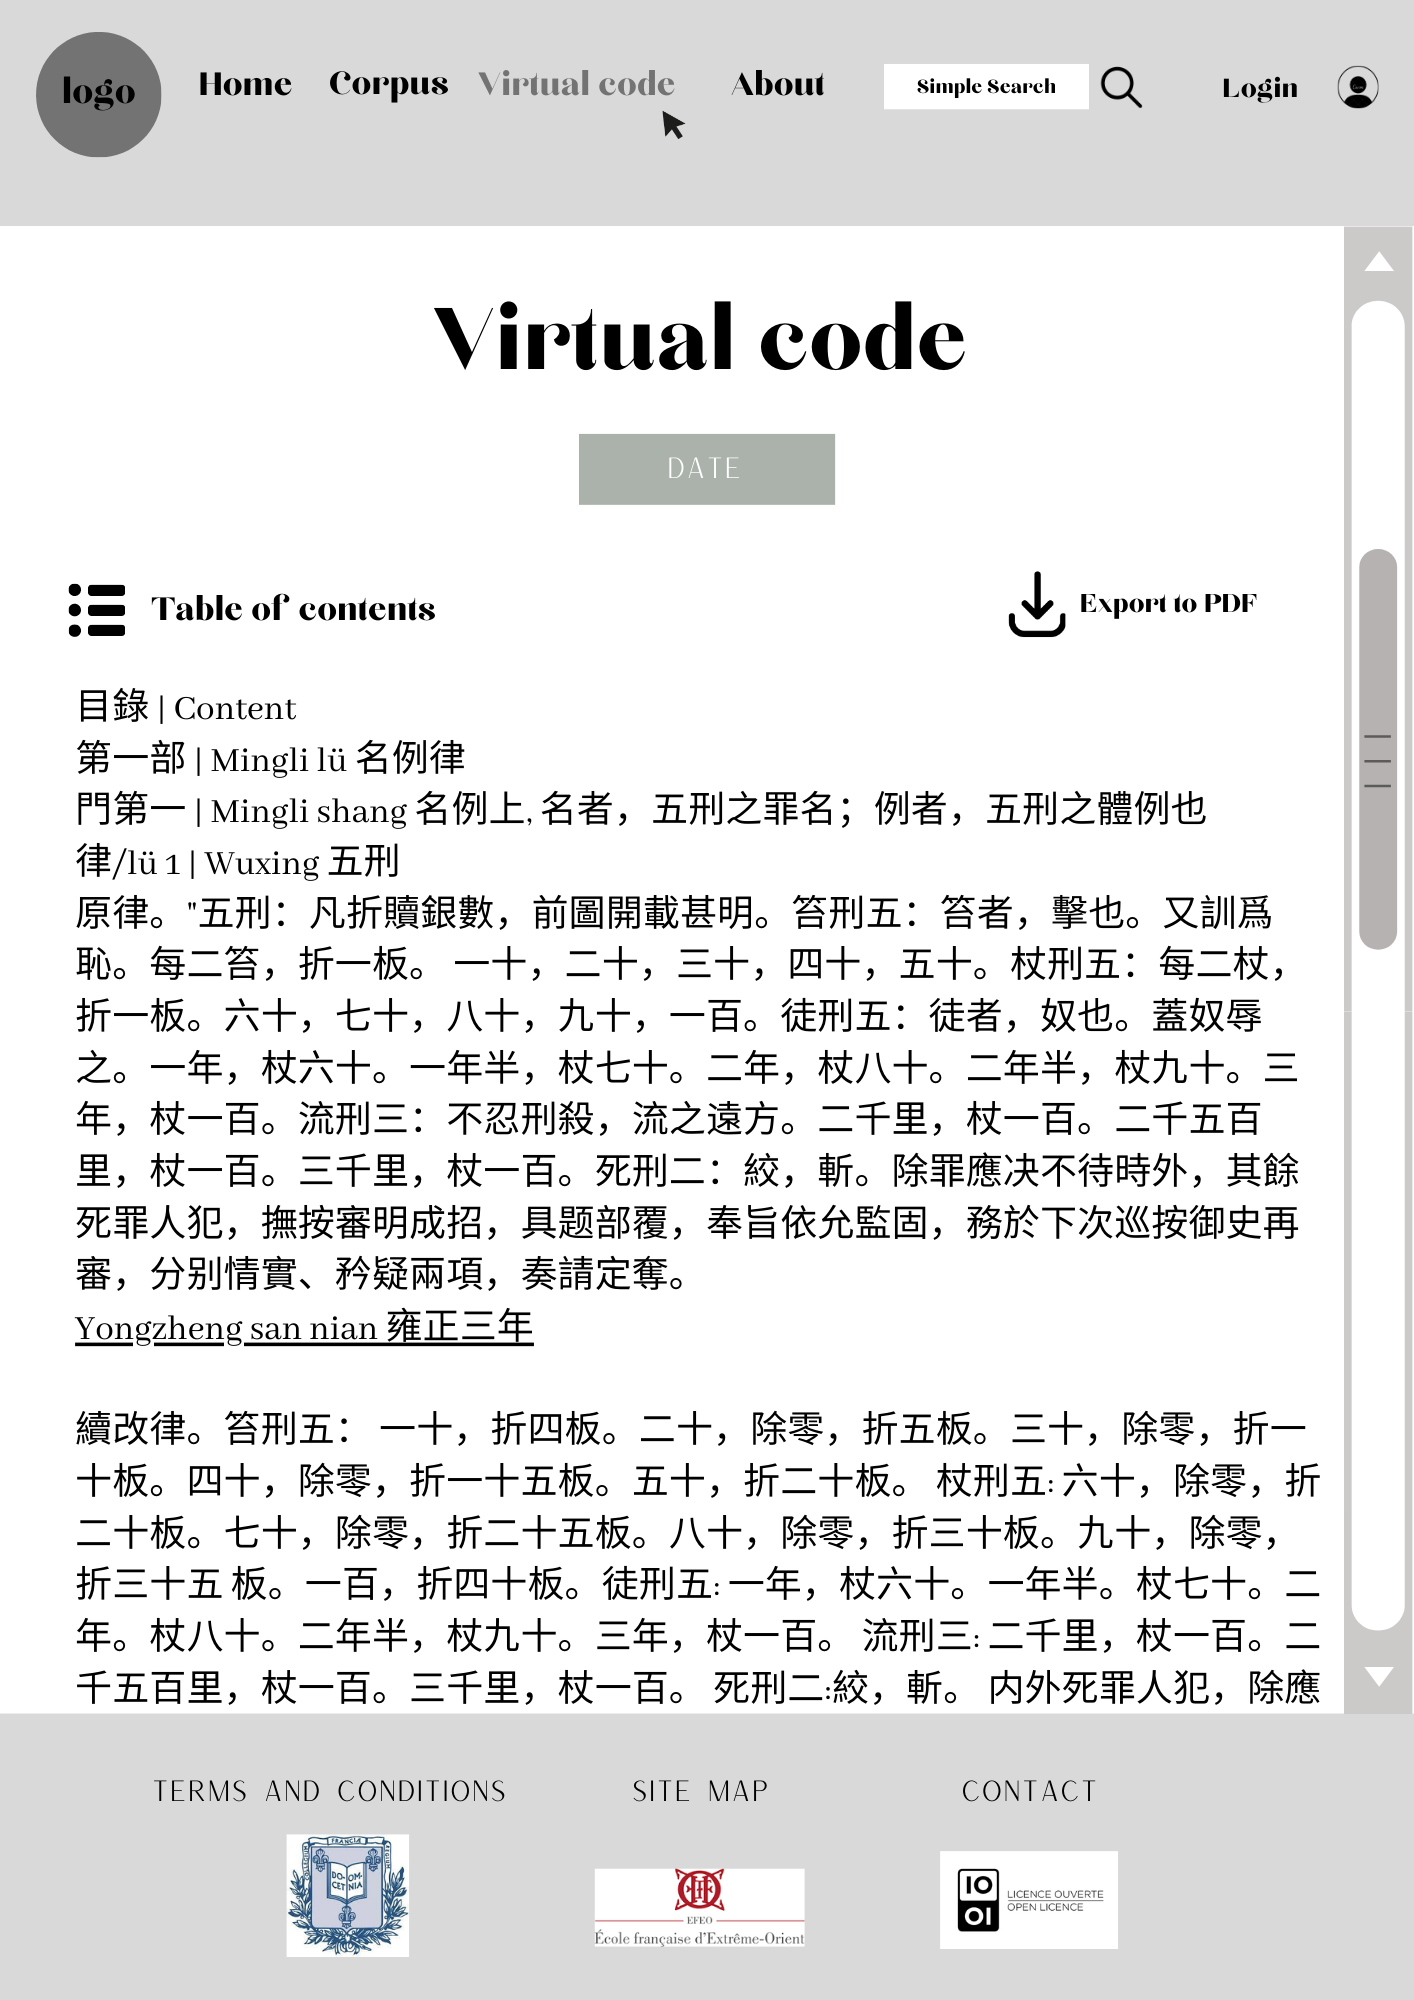
\includegraphics[width=\textwidth]{annexes/12 -Code virtuel (output).png}
\noindent 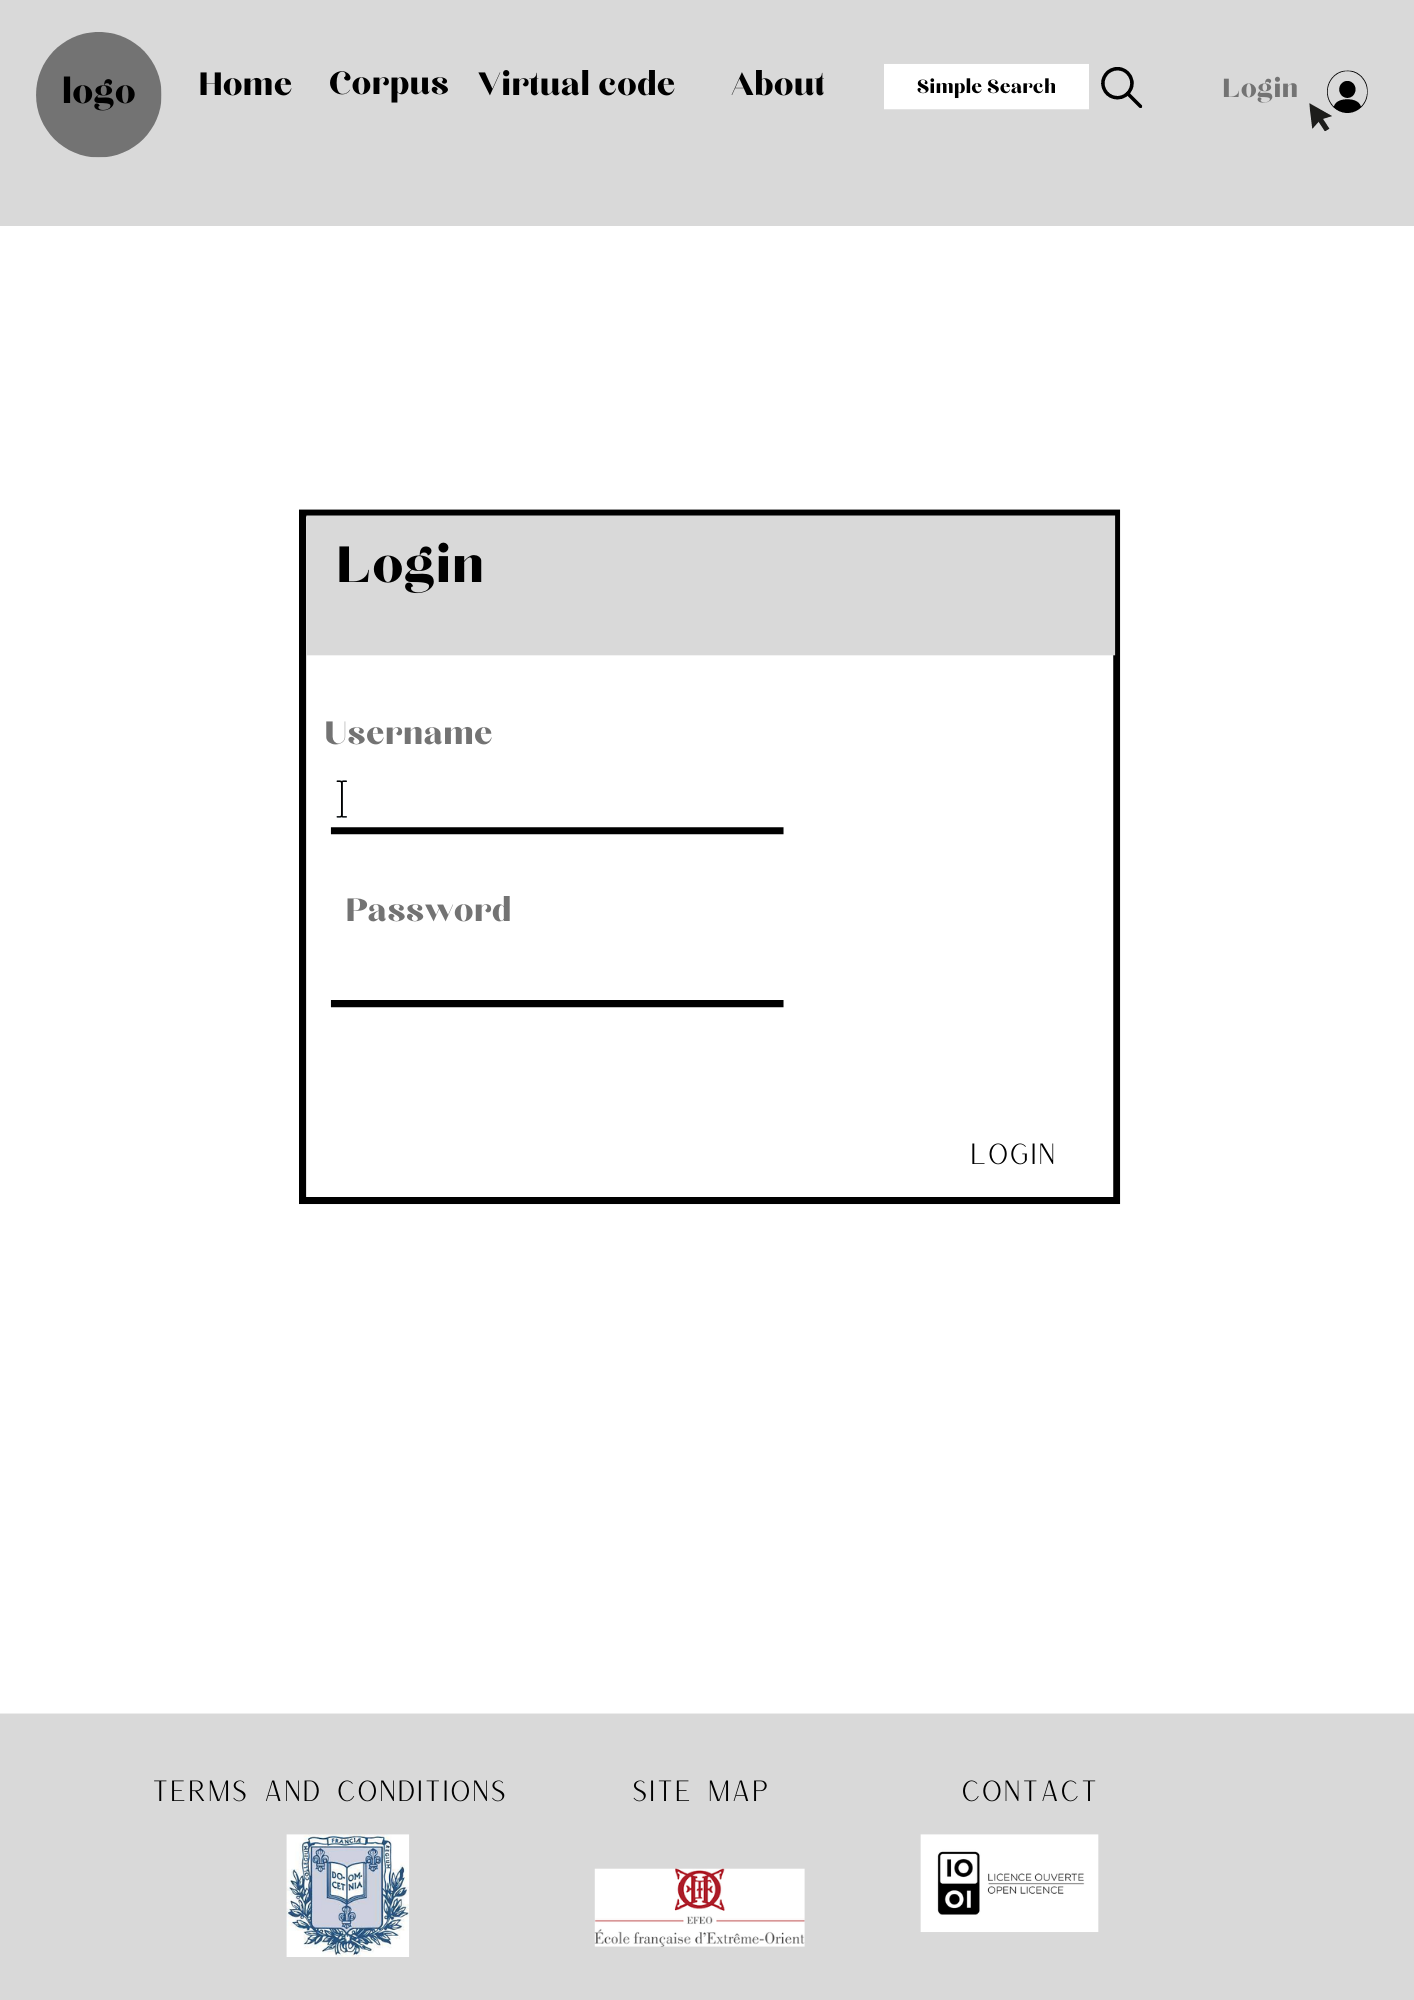
\includegraphics[width=\textwidth]{annexes/13 - Se connecter.png}
\noindent 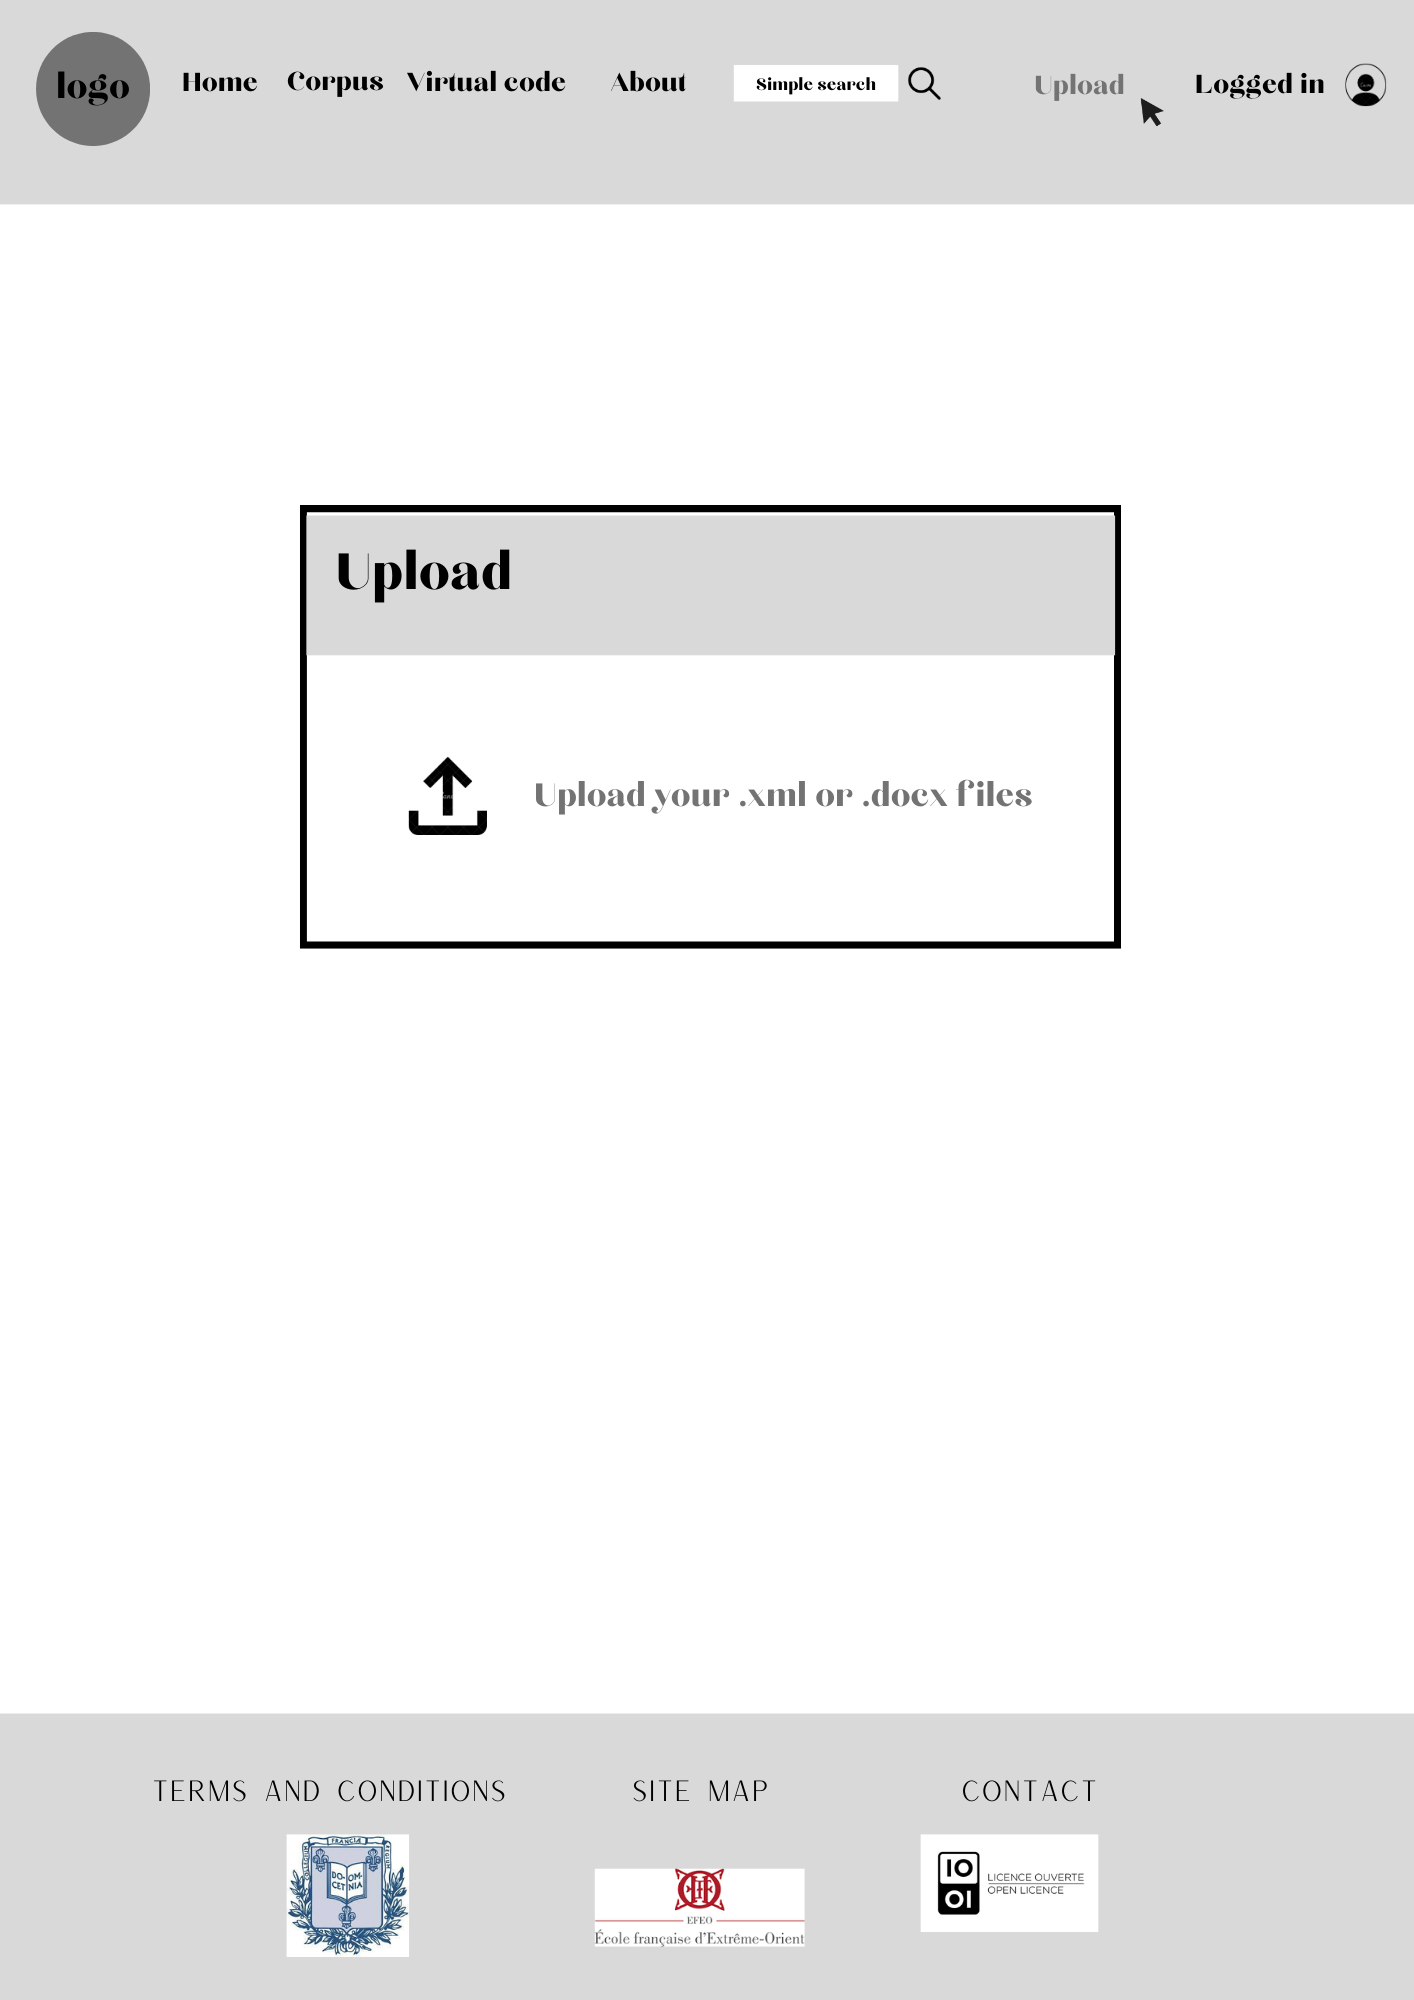
\includegraphics[width=\textwidth]{annexes/14 - Télécharger de nouveaux documents.png}

\section*{Liens}
\begin{itemize}
    \item 
\href{https://sharedocs.huma-num.fr/wl/?id=yHHcUPKWyusazIZqWVLgtbZI7J65OaLA&path=TEI%282%29&mode=grid}{Jeu de données \TEI de référence}
\item 
\href{}{Échantillon des données}
\item 
\href{https://sharedocs.huma-num.fr/wl/?id=yHHcUPKWyusazIZqWVLgtbZI7J65OaLA&path=ODD&mode=grid}{\ODD}
\item 
\href{}{\ODD pour l'affichage \tp}
\end{itemize}
\section*{Exemple d'affichage possible avec \tp}
\noindent 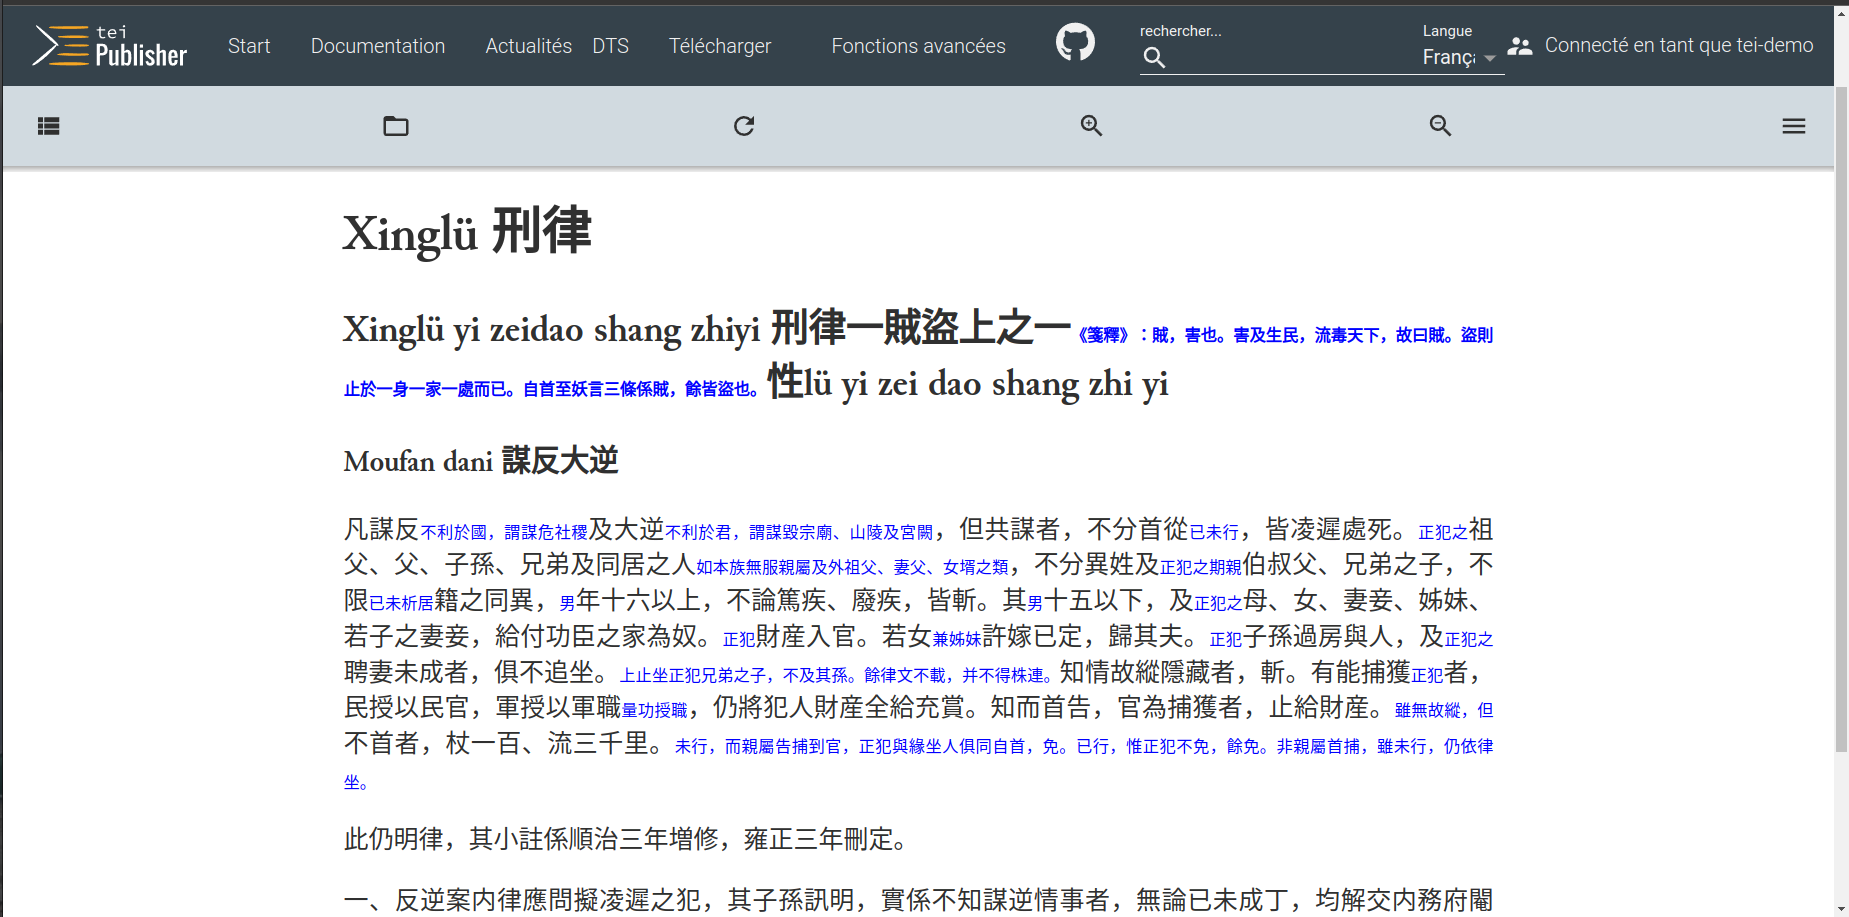
\includegraphics[width=\textwidth]{annexes/affichage.png}

\clearemptydoublepage

\backmatter
    \printacronyms[title=Liste des acronymes,toctitle=Acronymes]
    \addcontentsline{toc}{chapter}{\listfigurename}
    \listoffigures
    \printglossary 
    \printbibliography[keyword={histoire}, title={Histoire du droit chinois}]
    \printbibliography[keyword={edition}, title={Édition scientifique numérique}]
    \tableofcontents
	
\end{document}
